\documentclass[11pt,a4paper,dvipsnames]{article}
\usepackage[deliverable]{IOHKCoverPage}


\usepackage[margin=2.5cm]{geometry}
\usepackage{iohk}
\usepackage{microtype}
\usepackage{mathpazo} % nice fonts
\usepackage{amsmath}
\usepackage{amssymb}
\usepackage{amsthm}
\usepackage{latexsym}
\usepackage{mathtools}
\usepackage{stmaryrd}
\usepackage{extarrows}
\usepackage{slashed}
\usepackage[colon]{natbib}
\usepackage[unicode=true,pdftex,pdfa,colorlinks=true]{hyperref}
\usepackage{xcolor}
\usepackage[capitalise,noabbrev,nameinlink]{cleveref}
\usepackage{float}
\floatstyle{boxed}
\restylefloat{figure}
\usepackage{tikz}
\usepackage{booktabs}
\usepackage{enumerate}
\usepackage{fancyvrb}
\usepackage{xcolor}


%%
%% Package `semantic` can be used for writing inference rules.
%%
\usepackage{semantic}
%% Setup for the semantic package
\setpremisesspace{20pt}

% data for Deliverable header -- added by KH from an EU H2020 project template
\DeliverableNumber{GL-D1}
\DeliverableTitle{A Formal Specification of the Cardano Ledger with a Native Multi-Asset Implementation}
   {Formal Cardano Ledger with Multi-Asset Spec.}

\DeliverableResponsible{Formal Methods Team}

\DueDate{31$^{\textrm{st}}$ July 2020}

\SubmissionDate{20$^{\textrm{st}}$ August 2020}{20$^{\textrm{st}}$ August 2020}

\Authors{
   Polina Vinogradova \quad \texttt{polina.vinogradova@iohk.io} \\
   Andre Knispel \quad \texttt{andre.knispel@iohk.io}
}

\EditorName{Polina Vinogradova}
\LeaderName{Philipp Kant, \IOHK}
\InstitutionAddress{\IOHK}
\Version{1.0}
\Project{Goguen Ledger}
\DisseminationPU

%%
%% Types
%%
\newcommand{\Nothing}{\ensuremath{\Diamond}}
\newcommand{\N}{\ensuremath{\mathbb{N}}}
\newcommand{\Bool}{\type{Bool}}
\newcommand{\Npos}{\ensuremath{\mathbb{N}^{+}}}
\newcommand{\Z}{\ensuremath{\mathbb{Z}}}
\newcommand{\R}{\ensuremath{\mathbb{R}}}
\newcommand{\Rnn}{\ensuremath{\mathbb{R}^{\geq 0}}}
\newcommand{\Tx}{\type{Tx}}
\newcommand{\ShelleyTx}{\type{ShelleyTx}}
\newcommand{\GoguenTx}{\type{GoguenTx}}
\newcommand{\TxBody}{\type{TxBody}}
\newcommand{\UnsignedData}{\type{UnsignedData}}
\newcommand{\VldSR}{\type{VldSR}}
\newcommand{\VldOut}{\type{VldOut}}
\newcommand{\Vlds}{\type{Vlds}}
\newcommand{\TxWitness}{\type{TxWitness}}
\newcommand{\Ix}{\type{Ix}}
\newcommand{\RdmrPtr}{\type{RdmrPtr}}
\newcommand{\TxId}{\type{TxId}}
\newcommand{\Addr}{\type{Addr}}
\newcommand{\UTxO}{\type{UTxO}}
\newcommand{\UTxOIn}{\type{UTxOIn}}
\newcommand{\UTxOOut}{\type{UTxOOut}}
\newcommand{\Wdrl}{\type{Wdrl}}
\newcommand{\Coin}{\type{Coin}}
\newcommand{\PParams}{\type{PParams}}
\newcommand{\ShelleyPParams}{\type{ShelleyPParams}}
\newcommand{\NewParams}{\type{NewParams}}
\newcommand{\Slot}{\type{Slot}}
\newcommand{\SlotsPrior}{\ensuremath{\mathsf{SlotsPrior}}}
\newcommand{\SlotsPerEpoch}{\mathsf{SlotsPerEpoch}}
\newcommand{\SlotsPerKESPeriod}{\mathsf{SlotsPerKESPeriod}}
\newcommand{\SlotsStabilityParam}{\fun{k}}
\newcommand{\Duration}{\type{Duration}}
\newcommand{\StakePools}{\type{StakePools}}
\newcommand{\StakeDeleg}{\type{StakeDeleg}}
\newcommand{\StakeCreds}{\type{StakeCreds}}
\newcommand{\Seed}{\type{Seed}}
\newcommand{\seedOp}{\star}
\newcommand{\Ppm}{\type{Ppm}}
\newcommand{\Value}{\type{Value}}
\newcommand{\Integer}{\type{Integer}}
\newcommand{\ValMonoid}{\mathbf{TA}}
\newcommand{\ProtVer}{\ensuremath{\type{ProtVer}}}
\newcommand{\Language}{\type{Language}}
\newcommand{\ApName}{\ensuremath{\type{ApName}}}
\newcommand{\ApVer}{\ensuremath{\type{ApVer}}}
\newcommand{\SystemTag}{\ensuremath{\type{SystemTag}}}
\newcommand{\InstallerHash}{\ensuremath{\type{InstallerHash}}}
\newcommand{\PPUpdate}{\type{PPUpdate}}
\newcommand{\Applications}{\type{Applications}}
\newcommand{\AVUpdate}{\type{AVUpdate}}
\newcommand{\Update}{\type{Update}}
\newcommand{\DCert}{\type{DCert}}
\newcommand{\DCertRegKey}{\type{DCert_{regkey}}}
\newcommand{\DCertDeRegKey}{\type{DCert_{deregkey}}}
\newcommand{\DCertDeleg}{\type{DCert_{delegate}}}
\newcommand{\DCertRegPool}{\type{DCert_{regpool}}}
\newcommand{\DCertRetirePool}{\type{DCert_{retirepool}}}
\newcommand{\DCertGen}{\type{DCert_{genesis}}}
\newcommand{\DCertMir}{\type{DCert_{mir}}}
\newcommand{\PoolParam}{\type{PoolParam}}
\newcommand{\UTxOState}{\ensuremath{\type{UTxOState}}}
\newcommand{\SFState}{\ensuremath{\type{SFState}}}
\newcommand{\ledgerState}{\ensuremath{\type{ledgerState}}}
\newcommand{\ValEnv}{\type{ValEnv}}
\newcommand{\ValState}{\type{ValState}}
\newcommand{\ScrInData}{\type{ScrInData}}
\newcommand{\AddrRWD}{\type{Addr_{rwd}}}
\newcommand{\AddrB}{\type{Addr_{base}}}
\newcommand{\AddrP}{\type{Addr_{ptr}}}
\newcommand{\AddrE}{\type{Addr_{enterprise}}}
\newcommand{\AddrBS}{\type{Addr_{bootstrap}}}
\newcommand{\Ptr}{\type{Ptr}}
\newcommand{\DState}{\type{DState}}
\newcommand{\DWEnv}{\type{DWEnv}}
\newcommand{\DPSEnv}{\type{DPSEnv}}
\newcommand{\DPEnv}{\type{DPEnv}}
\newcommand{\DEnv}{\type{DEnv}}
\newcommand{\PEnv}{\type{PEnv}}
\newcommand{\DPState}{\type{DPState}}
\newcommand{\PState}{\type{PState}}
\newcommand{\DCertBody}{\type{DCertBody}}
\newcommand{\TData}{\type{TData}}
\newcommand{\DPoolReap}{\ensuremath{\type{poolreap}}}
\newcommand{\UPIState}{\type{UPIState}}
\newcommand{\UpdatePayload}{\type{UpdatePayload}}
\newcommand{\NetworkId}{\mathsf{NetworkId}}
\newcommand{\MemoryEstimate}{\type{MemoryEstimate}}

% multi-signature
\newcommand{\StakeCredential}{\type{Credential}_{stake}}
\newcommand{\StakeDelegs}{\type{StakeDelegs}}
\newcommand{\Quorum}{\type{Quorum}}

\newcommand{\txwitsVKey}[1]{\fun{txwitsVKey}~\var{#1}}
\newcommand{\txwitsScript}[1]{\fun{txwitsScript}~\var{#1}}

\newcommand{\AddrVKey}{\type{Addr^{vkey}}}
\newcommand{\AddrRWDVKey}{\type{Addr_{rwd}^{vkey}}}
\newcommand{\AddrRWDScr}{\type{Addr_{rwd}^{script}}}
\newcommand{\AddrVKeyB}{\type{Addr^{vkey}_{base}}}
\newcommand{\AddrVKeyP}{\type{Addr^{vkey}_{ptr}}}
\newcommand{\AddrVKeyE}{\type{Addr^{vkey}_{enterprise}}}
\newcommand{\AddrVKeyBS}{\type{Addr^{vkey}_{bootstrap}}}
\newcommand{\AddrScr}{\type{Addr^{script}}}
\newcommand{\AddrScrBase}{\type{Addr_{base}^{script}}}
\newcommand{\AddrScrEnterprise}{\type{Addr_{enterprise}^{script}}}
\newcommand{\AddrScrPtr}{\type{Addr_{ptr}^{script}}}
\newcommand{\AuxiliaryData}{\type{AuxiliaryData}}
\newcommand{\AuxiliaryDataHash}{\type{AuxiliaryDataHash}}
\newcommand{\Metadata}{\type{Metadata}}
\newcommand{\DataHash}{\type{DataHash}}
\newcommand{\ScriptHash}{\type{ScriptHash}}
\newcommand{\PolicyID}{\type{PolicyID}}
\newcommand{\AdaIDType}{\type{AdaIDType}}
\newcommand{\AdaID}{\type{AdaID}}
\newcommand{\PPHash}{\type{PPHash}}
\newcommand{\RdmrsHash}{\type{RdmrsHash}}
\newcommand{\Script}{\type{Script}}
\newcommand{\ScriptPlutus}{\type{Script}_{plc}}
\newcommand{\ScriptNI}{\type{Script^{native}_{v1}}}
\newcommand{\Timelock}{\type{Script^{native}_{v2}}}
\newcommand{\ScriptMSig}{\type{Script}_{msig}}
\newcommand{\ScriptV}{\type{Script_{v}}}
\newcommand{\Datum}{\type{Datum}}
\newcommand{\Rdmr}{\type{Rdmr}}
\newcommand{\CurItem}{\type{CurItem}}
\newcommand{\Rdmrs}{\type{Rdmrs}}
\newcommand{\DorR}{\type{DorR}}
\newcommand{\ValidationData}{\type{ValidationData}}
\newcommand{\IsValidating}{\type{IsValidating}}
\newcommand{\HashUnsData}{\type{HashUnsData}}
\newcommand{\True}{\type{True}}
\newcommand{\False}{\type{False}}
\newcommand{\MSig}{\type{MSig}}
\newcommand{\Credential}{\type{Credential}}
\newcommand{\AssetID}{\type{AssetID}}
\newcommand{\AssetName}{\type{AssetName}}
\newcommand{\Quantity}{\type{Quantity}}
\newcommand{\QuantityPM}{\type{Quantity}^{\pm}}
\newcommand{\ValuePM}{\type{Value}^{\pm}}

%% Adding witnesses
\newcommand{\TxIn}{\type{TxIn}}
\newcommand{\OutRef}{\type{OutRef}}
\newcommand{\ShelleyTxIn}{\type{ShelleyTxIn}}
\newcommand{\ShelleyTxOut}{\type{ShelleyTxOut}}
\newcommand{\ShelleyUTxO}{\type{ShelleyUTxO}}
\newcommand{\ShelleyChainState}{\type{ShelleyChainState}}
\newcommand{\HasDV}{\type{HasDV}}
\newcommand{\TxInScr}{\type{TxInScr}}
\newcommand{\Info}{\type{Info}}
\newcommand{\ExUnits}{\type{ExUnits}}
\newcommand{\CostMod}{\type{CostMod}}
\newcommand{\Prices}{\type{Prices}}
\newcommand{\ByteString}{\type{ByteString}}
\newcommand{\IsFee}{\type{IsFee}}
\newcommand{\TxOut}{\type{TxOut}}
\newcommand{\OutFoo}{\type{OutFoo}}
\newcommand{\TxOutND}{\type{TxOutND}}
\newcommand{\TxOutP}{\type{TxOutP}}
\newcommand{\VKey}{\type{VKey}}
\newcommand{\VKeyEv}{\type{VKey_{ev}}}
\newcommand{\VKeyGen}{\type{VKey_G}}
\newcommand{\SKey}{\type{SKey}}
\newcommand{\SKeyEv}{\type{SKey_{ev}}}
\newcommand{\KeyHash}{\type{KeyHash}}
\newcommand{\KeyHashGen}{\type{KeyHash_G}}
\newcommand{\KeyPair}{\type{KeyPair}}
\newcommand{\KeyPairEv}{\type{KeyPair_{ev}}}
\newcommand{\Sig}{\type{Sig}}
\newcommand{\Data}{\type{Data}}
%% Adding delegation
\newcommand{\Epoch}{\type{Epoch}}
\newcommand{\KESPeriod}{\type{KESPeriod}}
%% Blockchain
\newcommand{\Gkeys}{\var{G_{keys}}}
\newcommand{\Block}{\type{Block}}
\newcommand{\SlotId}{\type{SlotId}}
\newcommand{\PPUpdateEnv}{\type{PPUpdateEnv}}
\newcommand{\AVUpdateEnv}{\type{AVUpdateEnv}}
\newcommand{\AVUpdateState}{\type{AVUpdateState}}
\newcommand{\UpdateEnv}{\type{UpdateEnv}}
\newcommand{\UpdateState}{\type{UpdateState}}
\newcommand{\UTxOEnv}{\type{UTxOEnv}}
\newcommand{\CEEnv}{\type{CEEnv}}
\newcommand{\CEState}{\type{CEState}}
\newcommand{\BDEnv}{\type{BDEnv}}
\newcommand{\BDState}{\type{BDState}}
\newcommand{\LEnv}{\type{LEnv}}
\newcommand{\LState}{\type{LState}}
\newcommand{\GoguenChainState}{\type{GoguenChainState}}
%%
%% Functions
%%
\newcommand{\txins}[1]{\fun{txins}~ \var{#1}}
\newcommand{\txouts}[1]{\fun{txouts}~ \var{#1}}
\newcommand{\txcerts}[1]{\fun{txcerts}~ \var{#1}}
\newcommand{\txid}[1]{\fun{txid}~ \var{#1}}
\newcommand{\outs}[1]{\fun{outs}~ \var{#1}}
\newcommand{\values}[1]{\fun{values}~ #1}
\newcommand{\ubalance}[1]{\fun{ubalance}~ \var{#1}}
\newcommand{\txttl}[1]{\fun{txttl}~ \var{#1}}
\newcommand{\firstSlot}[1]{\fun{firstSlot}~ \var{#1}}
\newcommand{\totalDeposits}[3]{\fun{totalDeposits}~ \var{#1} ~ \var{#2} ~ \var{#3}}
\newcommand{\decayedKey}[4]{\fun{decayedKey}~ \var{#1}~ \var{#2}~ \var{#3}~ \var{#4}}
\newcommand{\decayedTx}[3]{\fun{decayedTx}~ \var{#1}~ \var{#2}~ \var{#3}}
\newcommand{\keyRefund}[6]{\fun{keyRefund}~ {#1}~{#2}~{#3}~\var{#4}~\var{#5}~\var{#6}}
\newcommand{\refund}[4]{\fun{refund}~ \var{#1}~ \var{#2}~ {#3}~ {#4}}
\newcommand{\keyRefunds}[2]{\fun{keyRefunds}~ \var{#1}~ \var{#2}}
\newcommand{\consumed}[2]{\fun{consumed}~ \var{#1}~ \var{#2}}
\newcommand{\produced}[2]{\fun{produced}~ \var{#1}~ \var{#2}}
\newcommand{\applyFun}[2]{\fun{#1}~\var{#2}}

\newcommand{\RegKey}[1]{\textsc{RegKey}(#1)}
\newcommand{\DeregKey}[1]{\textsc{DeregKey}(#1)}
\newcommand{\Delegate}[1]{\textsc{Delegate}(#1)}
\newcommand{\RegPool}[1]{\textsc{RegPool}(#1)}
\newcommand{\RetirePool}[1]{\textsc{RetirePool}(#1)}
\newcommand{\cwitness}[1]{\fun{cwitness}~ \var{#1}}
\newcommand{\dpool}[1]{\fun{dpool}~ \var{#1}}
\newcommand{\poolParam}[1]{\fun{poolParam}~ \var{#1}}
\newcommand{\retire}[1]{\fun{retire}~ \var{#1}}
\newcommand{\addrRw}[1]{\fun{addr_{rwd}}~ \var{#1}}
\newcommand{\epoch}[1]{\fun{epoch}~\var{#1}}
\newcommand{\kesPeriod}[1]{\fun{kesPeriod}~\var{#1}}

%% UTxO witnesses
\newcommand{\inputs}[1]{\fun{inputs}~ \var{#1}}
\newcommand{\txwits}[1]{\fun{txwits}~ \var{#1}}
\newcommand{\verify}[3]{\fun{verify} ~ #1 ~ #2 ~ #3}
\newcommand{\sign}[2]{\fun{sign} ~ #1 ~ #2}
\newcommand{\verifyEv}[4]{\fun{verify_{ev}} ~ #1 ~ #2 ~ #3 ~ #4}
\newcommand{\signEv}[3]{\fun{sign_{ev}} ~ #1 ~ #2 ~ #3}
\newcommand{\serialised}[1]{\llbracket \var{#1} \rrbracket}
\newcommand{\hashKey}[1]{\fun{hashKey}~ \var{#1}}
\newcommand{\txbody}[1]{\fun{txbody}~ \var{#1}}
\newcommand{\txfee}[1]{\fun{txfee}~ \var{#1}}
\newcommand{\txwdrls}[1]{\fun{txwdrls}~ \var{#1}}
\newcommand{\minfee}[2]{\fun{minfee}~ \var{#1}~ \var{#2}}
\newcommand{\slotminus}[2]{\var{#1}~-_{s}~\var{#2}}
\DeclarePairedDelimiter\floor{\lfloor}{\rfloor}
% wildcard parameter
\newcommand{\wcard}[0]{\underline{\phantom{a}}}
%% Adding ledgers...
\newcommand{\utxo}[1]{\fun{utxo}~ #1}
%% Delegation
\newcommand{\delegatesName}{\fun{delegates}}
\newcommand{\delegates}[3]{\delegatesName~#1~#2~#3}
\newcommand{\dwho}[1]{\fun{dwho}~\var{#1}}
\newcommand{\depoch}[1]{\fun{depoch}~\var{#1}}
\newcommand{\dval}{\ensuremath{d_{\mathsf{val}}}}
%% Delegation witnesses
\newcommand{\dbody}[1]{\fun{dbody}~\var{#1}}
\newcommand{\dwit}[1]{\fun{dwit}~\var{#1}}
%% Blockchain
\newcommand{\bwit}[1]{\fun{bwit}~\var{#1}}
\newcommand{\bslot}[1]{\fun{bslot}~\var{#1}}
\newcommand{\bbody}[1]{\fun{bbody}~\var{#1}}
\newcommand{\bhbody}[1]{\fun{bhbody}~\var{#1}}
\newcommand{\bdlgs}[1]{\fun{bdlgs}~\var{#1}}
%% ledgerstate constants
\newcommand{\genesisId}{\ensuremath{Genesis_{Id}}}
\newcommand{\genesisTxOut}{\ensuremath{Genesis_{Out}}}
\newcommand{\genesisUTxO}{\ensuremath{Genesis_{UTxO}}}
\newcommand{\genesisUTxOState}{(\genesisUTxO,\wcard,\wcard,\wcard)}
\newcommand{\emax}{\ensuremath{\mathsf{E_{max}}}}

\newcommand{\unitInterval}{\ensuremath{[0,~1]}}
\newcommand{\unitIntervalNonNull}{\ensuremath{(0,~1]}}
\newcommand{\nonnegReals}{\ensuremath{[0,~\infty)}}
\newcommand{\posReals}{\ensuremath{(0,~\infty)}}

\theoremstyle{definition}
\newtheorem{definition}{Definition}[section]
\newtheorem{lemma}[definition]{Lemma}
\newtheorem{theorem}[definition]{Theorem}
\newtheorem{property}{Property}[section]

\newcommand{\leteq}{\ensuremath{\mathrel{\mathop:}=}}

\newcommand{\arrow}{\rightarrow}

\definecolor{hldiffcolor}{rgb}{0.95, 0.93, 0}
\newcommand{\hldiff}[1]{\mathchoice
  {\colorbox{hldiffcolor}{$\displaystyle#1$}}
  {\colorbox{hldiffcolor}{$\textstyle#1$}}
  {\colorbox{hldiffcolor}{$\scriptstyle#1$}}
  {\colorbox{hldiffcolor}{$\scriptscriptstyle#1$}}}
\DeclareMathOperator{\supp}{supp}

\newcommand{\khcomment}[1]{\textbf{ -- KH: #1 -- }}
\renewcommand{\khcomment}[1]{} % For publication

\begin{document}

\hypersetup{
  pdftitle={A Formal Specification of the Cardano Ledger},
  breaklinks=true,
  bookmarks=true,
  colorlinks=false,
  linkcolor={blue},
  citecolor={blue},
  urlcolor={blue},
  linkbordercolor={white},
  citebordercolor={white},
  urlbordercolor={white}
}

  \cleardoublepage%
  \tableofcontents%

  \listoffigures%
  \clearpage%

  \begin{changelog}
        \change{2019/10/08}{Jared Corduan, Polina Vinogradova and Matthias G\"udemann}{FM (IOHK)}{Initial version (0.1).}
        \change{2019/10/08}{Kevin Hammond}{FM (IOHK)}{Added cover page.}
        \change{2020/11/17}{Jared Corduan}{FM (IOHK)}
          {Removed unused deliverable outline image,
           set version to 1.0,
           and changed the reward calculation so that $\eta$
             takes $d$ into account.}
        \change{2021/05/17}{Jared Corduan}{FM (IOHK)}{Added Example Illustration.}
        \change{2021/06/14}{Jared Corduan}{FM (IOHK)}
          {Added an errata section,
           fixed a typo in leader check and in the LEDGERS rule index,
           and synced the reward calculation with the implementation}
        \change{2021/06/17}{Jared Corduan}{FM (IOHK)}
          {Allow the pool influence parameter $a_0$ to be zero,
          remove all mentions of deposit decay, sync varibale names with code.}
        \change{2021/08/27}{Jared Corduan}{FM (IOHK)}{Fixed definitions in the header-only validation properties.
          CHAIN transition did not need to use previous protocol parameters.}
        \change{2021/10/08}{Jared Corduan}{FM (IOHK)}{The function createRUpd
          should get the pool parameters from the go snapshot.
          The TICKN rule was missing from the dependency diagram.}
        \change{2021/11/08}{Jared Corduan}{FM (IOHK)}{Fixed typo in the description of variable length encodings.}
        \change{2021/12/13}{Jared Corduan}{FM (IOHK)}{Re-wrote the MIR transitions to be more compact.}
      \end{changelog}
      \clearpage%
\renewcommand{\thepage}{\arabic{page}}
\setcounter{page}{1}

\title{A Formal Specification of the Cardano Ledger}

\author{Jared Corduan  \\ {\small \texttt{jared.corduan@iohk.io}} \\
   \and Polina Vinogradova \\ {\small \texttt{polina.vinogradova@iohk.io}} \\
   \and Matthias G\"udemann  \\ {\small \texttt{matthias.gudemann@iohk.io}}}

%\date{}

\maketitle

\begin{abstract}
This document provides a formal specification of the Cardano ledger for use in the upcoming Shelley implementation.
It is intended to underpin a Haskell executable specification that will be the basis of the initial
Shelley release, and represents a core design and quality assurance document.
It will be used to define properties and tests, and to provide the basis for strong formal assurance
using mathematical proof techniques.
The document defines the rules for extending the ledger with transactions
that will affect both UTxO and stake delegation.
Key properties that have been identified include the preservation of balances, absence of double spend, stakepool registration,
and reward splitting.
\end{abstract}

\section*{List of Contributors}
\label{acknowledgements}

Nicol\'as Arqueros,
Dan Bornside,
Nicholas Clarke,
Duncan Coutts,
Ruslan Dudin,
Sebastien Guillemot,
Kevin Hammond,
Vincent Hanquez,
Ru Horlick,
Michael Hueschen,
Christian Lindgren,
Yun Lu,
Philipp Kant,
Jean-Christophe Mincke,
Damian Nadales,
Ashish Prajapati,
Nicolas Di Prima,
Andrew Westberg.


\pagebreak
\tableofcontents
\listoffigures

\section{Introduction}

Currently still todo:

\begin{itemize}
\item Adjust TxInfo
\item Update minUTxO
\end{itemize}

This specification describes the incremental changes from the Alonzo
era of Cardano to the Babbage era. The main objective of this era is
to make small adjustments in many places, usually to simplify the
ledger or to include features that didn't make it into past eras. As
part of this effort, we also make some changes to the notation used in
these specifications, which should make them easier to understand and
maintain.

Concretely, this specification makes the following changes:
\begin{itemize}
\item Add reference inputs to transactions
\item Add inline datums in the UTxO
\item Add reference scripts
\item Add transaction fields for specifying and returning collateral
\item Remove the protocol parameters $\var{d}$ and $\var{extraEntropy}$
\item Remove the overlay schedule
\item Block headers to only include a single VRF value and proof
\item Remove the pre-filtering of unregistered stake credentials in the reward calculation
\end{itemize}

\section{Notation}

In addition to the notation in the Shelley spec, we use the following notations:

\begin{description}
\item[Functions with finite support] For a monoid $M$, $A \to_0 M$
  are the functions $f : A \to M$ with finite support, i.e. such that
  there exist only finitely many $a \in A$ such that $f a \neq 0$. We
  denote the support of $f$ by $\supp f$, which is defined as
  $\supp f := \{ a \in A : f a \neq 0 \}$.
\end{description}

\section{Coin and Multi-Asset Bundles}
\label{sec:coin-ma}

In this chapter we introduce an algebraic structure, $\ValMonoid$,
which we define to be a partially ordered abelian group with several additional functions.
The group structure and additional functions represent the
features required in order to treat elements as \emph{assets} (or bundles thereof),
which includes the ability to do certain accounting operations on them (addition, etc.),
as well as some other operations (see below).
These operations are used to describe the ShelleyMA transaction processing rules
without fixing a concrete underlying $\ValMonoid$.

In order to give a concrete ledger specification, a specific type
endowed with $\ValMonoid$ structure must be used in its place.
Depending on the concrete type selected for this purpose,
we obtain distinct ledgers. In particular, we get

\begin{itemize}
  \item the Allegra ledger rules with $\Coin$, and
  \item the Mary ledger rules with $\Value$ (a type that represents a heterogeneous collection of assets via
  single element)
\end{itemize}

Below we give the definitions of all the functions that must be defined on
$\Coin$ and $\Value$ in order for them to have the structure of a $\ValMonoid$.
In Section \ref{sec:other-valmonoids} we give several other types which we can meaningfully
support the definition of the required functions (addition, size, etc.), including
an optimized representation that more accurately represents the ledger implementation
of the multi-asset type.
These types are convertible to and from the $\Value$ type, and appear in other
parts of the system as a multi-asset representation which is more suitable in particular
usecases.

\subsection{$\ValMonoid$}

Figure \ref{fig:ValMonoid} gives names and types of functions which
make up the $\ValMonoid$ structure. The functions $\fun{zero}$ and $(+)$ are
part of the abelian group structure, but we include them here to give the
complete $\ValMonoid$ structure. The partial order is given by $\fun{pointwise}~\leq$.

Note that we use overloaded notation
for partial order comparisons of $\ValMonoid$ elements elsewhere in the spec. That is,
we use the comparison operators $=,~<,~>,~\leq,~\geq$ in place the following pointwise comparisons, respectively

\[ \fun{pointwise}~(=),~\fun{pointwise}~(<),~\fun{pointwise}~(>),~\fun{pointwise}~(\leq),~\fun{pointwise}~(\geq) \]

%%
%% Figure ValMonoid and its Functions
%%
\begin{figure}[htb]
  \begin{align*}
      & \mathsf{ValType} ~\in~ \mathsf{Type}  \\
      & \text{A type}
      \nextdef
      %
      & \fun{zero} ~\in~ \mathsf{ValType} \\
      & \text{Additive identity of $\mathsf{ValType}$}
      \nextdef
      %
      & (+) ~\in~ \mathsf{ValType} \to \mathsf{ValType} \to \mathsf{ValType}\\
      & \text{Addition on $\mathsf{ValType}$}
      \nextdef
      %
      & (*) ~\in~ \mathsf{Integer} \to \mathsf{ValType} \to \mathsf{ValType}\\
      & \text{Scale $\mathsf{ValType}$ value by integral constant}
      \nextdef
      %
      & \fun{coin} ~\in~ \mathsf{ValType} \to \Coin\\
      & \text{Return the Ada contained inside the $\mathsf{ValType}$ element}
      \nextdef
      %
      & \fun{inject} ~\in~ \Coin \to \mathsf{ValType}\\
      & \text{Create a $\mathsf{ValType}$ element containing only this amount of Ada}
      \nextdef
      %
      & \fun{adaOnly} ~\in~ \mathsf{ValType} \to \Bool \\
      & \fun{adaOnly} =
        \begin{cases}
          \True & \fun{inject} \circ \fun{coin}~ = ~\fun{id}_{\mathsf{ValType}} \\
          \False & \text{otherwise}
        \end{cases} \\
      & \text{Check if a given $\mathsf{ValType}$ element contains only Ada}
      \nextdef
      %
      & \fun{size} ~\in~ \mathsf{ValType} \to \MemoryEstimate\\
      & \text{Return the size, in words, of a $\mathsf{ValType}$ element}
      \nextdef
      %
      & \fun{pointwise} ~\in~ (\Integer \to \Integer \to \Bool) \to (\mathsf{ValType} \to \mathsf{ValType} \to \Bool)\\
      & \text{Pointwise comparison of two $\mathsf{ValType}$ elements}
  \end{align*}
  \caption{The $\ValMonoid$ Structure}
  \label{fig:ValMonoid}
\end{figure}

\subsection{$\Coin$ in the Allegra era}

For the Allegra era, we require the $\ValMonoid$ asset representation to support
only a single asset, Ada, represented via $\Coin$. This section defines the
$\ValMonoid$ functions for the $\Coin$ type, see Figure
\ref{fig:coin}. Addition and multiplication are defined in the usual way
(as on $\Integer$).

When multi-asset support on the ledger is introduced, Ada ($\Coin$) will still be
the most common type of asset on the ledger, as the ledger rules enforce that
some quantity of it (specified via
the $\fun{coinsPerUTxOWord}$ protocol parameter) must
be contained in every UTxO on the ledger.
It is the only
type of asset that can be used for all non-UTxO ledger accounting, including deposits,
fees, rewards, treasury, and the proof of stake protocol. For this reason, not
all occurrences of $\Coin$ inside a transaction or in the ledger state can or
should be replaced with the abstract $\ValMonoid$.

For the Allegra version of the function $\fun{policies}$, which operates on $\Coin$ as the
$\ValMonoid$. No policies are associated with $\Coin$, since minting of Ada is not allowed.

%%
%% Figure Coin Functions
%%
\begin{figure}[htb]
  \begin{align*}
      & \fun{policies} ~=~ \Nothing
      \nextdef
      & \fun{zero} ~=~ 0
      \nextdef
      %
      & \fun{coin} ~=~ \fun{id}_{\Coin}
      \nextdef
      %
      & \fun{inject} ~=~ \fun{id}_{\Coin}
      \nextdef
      %
      & \fun{size}~\wcard ~=~ 0
      \nextdef
      %
      & \fun{pointwise} ~=~ \fun{id}_{(\Integer \to \Integer \to \Bool)}
  \end{align*}
  \caption{$\ValMonoid$ structure with $\Coin$}
  \label{fig:coin}
\end{figure}



\noindent \textbf{Relation between $\fun{inject}$ and $\fun{coin}$.}
When composed as

\[\fun{coin} \circ \fun{inject} = \fun{id}_{\Coin}\]

these functions give the identity on $\Coin$, but composed in the opposite order as

\[\fun{inject} \circ \fun{coin}\]

they return an element of $\ValMonoid$ containing only the Ada contained in the original $\ValMonoid$ element.

\subsection{Multi-assets and $\Value$ in the Mary Era}

Elements of $\Value$ represent heterogeneous collections of assets,
both user-defined, and Ada. The Mary era ledger fixes the underlying $\ValMonoid$ to
$\Value$ in order to introduce multi-asset support.
This section describes the type $\Value$, the operations required on
it, its relation to $\Coin$. It also as gives the definitions of the
$\ValMonoid$ functions for $\Value$.

Figure \ref{fig:defs:value} introduces the basic types that make up the $\Value$ type,
as well as defining the functions required to for $\Value$ to be a $\ValMonoid$.

\begin{figure*}[t!]
  \emph{Derived types}
  %
  \begin{equation*}
    \begin{array}{r@{~\in~}l@{\qquad=\qquad}lr}
      \var{aname} & ~\AssetName & \mathsf{ByteString} \\
      \var{pid} & \PolicyID & \ScriptHash \\
      \var{adaID} & ~\AdaIDType & \{~\mathsf{AdaID}~\} \\
      \var{aid} & \AssetID & \AdaIDType \uniondistinct (\PolicyID \times \AssetName) \\
      \var{quan} & \Quantity & \Z \\
      \var{v}, \var{w} & \Value & \AssetID \mapsto_0 \Quantity
    \end{array}
  \end{equation*}
  %
  \emph{$\ValMonoid$ and auxiliary functions for $\Value$}
  %
  \begin{align*}
    & \fun{policies} ~\in~ \Value \to \powerset{\PolicyID} \\
    & \fun{policies}~v ~=~ \{~\var{pid}~\vert~(\var{pid,~\wcard})~\in~\supp{~v}~\}
    \nextdef
    %
    & \fun{anames} ~\in~ \Value \to \powerset{\AssetName} \\
    & \fun{anames}~v ~=~ \{~\var{aname}~\vert~(\var{\wcard,~aname})~\in~\supp{~v}~\}
    \nextdef
    %
    & \fun{zero} ~=~ \Nothing
    \nextdef
    %
    & \fun{coin}~\var{v} ~=~ \var{v}~\mathsf{AdaID}
    \nextdef
    %
    & \fun{inject}~c  ~=~ \mathsf{AdaID}~\mapsto_0~\var{c}
    \nextdef
    %
    & \fun{size} ~~~ \text{see Section \ref{sec:value-size}}
  \end{align*}
  \caption{$\ValMonoid$ Function Definitions and Auxiliary Functions for Value}
  \label{fig:defs:value}
\end{figure*}

\begin{itemize}
  \item $\PolicyID$ identifies monetary policies. A policy ID $\var{pid}$ is associated with a script
    $s$ such that $\fun{hashScript}~s~=~pid$. When a transaction attempts to create or destroy assets
    that fall under the policy ID $\var{pid}$,
    $s$ verifies that the transaction
    respects the restrictions that are imposed by the monetary policy.
    See sections \ref{sec:transactions} and \ref{sec:utxo} for details.

  \item $\AssetName$ is a byte string used to distinguish different assets with the same $\PolicyID$.
    Each $aname$ identifies a particular kind of asset out of all the assets under the
    $\var{pid}$ policy (but not necessarily among assets under other policies).
    The maximum length of this
    byte string is 32 bytes (this is not explicitly enforced in this spec).

  \item $\AssetID$ is either $\mathsf{AdaID}$ or a pair of a policy ID and an asset name.
  It is a unique and permanent
  identifier of an asset. That is, there are is no mechanism to change it or
  any part of it for any assets.

  Mary MA assets are fungible with each other if and only if they have to the same $\AssetID$.
  The reason the unique identifier is a pair of two elements (except for the non-mintable Ada case) is to allow
  minting arbitrary collections of unique assets under a single policy.

  \item $\mathsf{AdaID}$ is a special asset ID for Ada, different than all other asset IDs.
  It is a term of the single-term type $\AdaIDType$.
  It does not include a policy, so instead, the validation outcome in the presence
  of Ada in the $\fun{mint}$ field of the transaction is specified in the UTXO
  ledger rule. The rule disallows the $\fun{mint}$ field to contain Ada.

  \item $\Quantity$ is an integer type that represents an amount of a specific $\AssetName$. We associate
    a $q\in\Quantity$ with a specific asset to track how much of that asset is contained in a given asset value.

  \item $\Value$ is the multi-asset type that is used to represent
    a collection of assets, including Ada. This type is a finitely supported map.

    If $\var{aid}$ is an $\AssetID$ and $v \in \Value$,
    the quantity of assets with that assed ID contained in $v$ is $v~\var{aid}$.
    Elements of $\Value$ are sometimes also referred to as
    \emph{asset bundles}.

  \item $\fun{inject}$ takes a $\Coin$ amount and returns a $\Value$ containing
  that amount of Ada, ie. assets associated with the $\mathsf{AdaID}$ asset ID.

  \item $\fun{coin}$ returns the amount of Ada contained in an element of $\Value$ (ie.
  the amount of assets associated with the $\mathsf{AdaID}$ asset ID).
\end{itemize}

\noindent \textbf{Special Ada representation.}
Although all assets are native on the Cardano ledger (ie. the accounting and
transfer logic for them is done directly by the ledger), Ada is still treated in a
special way by the ledger rules, and is the most common type of asset on the ledger.
It can
be used for special purposes (such as fees) for which other assets cannot be used.
The underlying consensus algorithm relies on Ada in a way that
cannot be extended to user-defined assets.
Ada can also neither be minted nor burned.

Note that in the $\Value$ definition above, we pick a special asset ID for Ada, that
is not part of the type which represents the asset IDs for all other assets.
Combining the asset name and policy for Ada gives a type-level guarantee that there is exactly
one kind of asset that is associated with it in any way, rather than
deriving this guarantee as an emergent property of minting rules.

Additionally, not giving Ada an actual policy ID
(that could have a hash-associated policy) eliminates the possibility
certain cryptographic attacks.
We sometimes refer to Ada as the primary or principal currency. Ada does not,
for the purposes of the Mary ledger spec, have a $\PolicyID$ or an $\AssetName$.

\subsection{Pointwise Value Operations and Partial Order}

We have a number of operations on $\Value$ left to define for it to have
$\ValMonoid$ structure. These are binary relations, addition, and
scalar multiplication. These are all done
pointwise in accordance with the usual definitions of these operations on
finitely supported maps, see Figure \ref{fig:pointwise}.

\begin{figure*}[t!]
  \begin{align*}
    & v~+~w =& \{~ aid~\mapsto_0 ~((v~\var{aid})~*~(w~\var{aid})) ~\vert~ \var{aid} \in (\fun{dom}~v)\cup(\fun{dom}~w) ~\}
    \nextdef
    %
    & q~*~v =& \{~ aid~\mapsto_0 ~(q~*~(v~\var{aid})) ~\vert~ \var{aid} \in \fun{dom}~v~\}
    \nextdef
    %
    & \fun{pointwise}~R~v~w =& \forall~\var{aid} ~\in ~(\fun{dom}~v~\cup~\fun{dom}~w),~R~(v~\var{aid})~(w~\var{aid})
  \end{align*}
  \caption{Pointwise operations on Value}
  \label{fig:pointwise}
\end{figure*}

\section{Transactions}
\label{sec:transactions}
\begin{figure*}[htb]
  \emph{Derived Types}
  %
  \begin{equation*}
    \begin{array}{l@{\qquad=\qquad}lr}
      \TxOut & \Addr \times \Value \times (\hldiff{\Datum} \uniondistinct \DataHash)^? \times \hldiff{\Script^?}
    \end{array}
  \end{equation*}
  % 
  \emph{Transaction Types}
  %
  \begin{equation*}
    \begin{array}{r@{~~}l@{~~}l@{\qquad}l}
      \TxBody ~=~
      & \powerset{\TxIn} & \fun{spendInputs}& \text{Inputs}\\
      & \times ~\powerset{\TxIn} & \fun{collInputs} & \text{Collateral inputs}\\
      & \times ~\hldiff{\powerset{\TxIn}} & \hldiff{\fun{refInputs}} & \hldiff{\text{Reference inputs}}\\
      & \times ~(\Ix \pto \TxOut) & \fun{txouts}& \text{Outputs}\\
      & \times ~\hldiff{\TxOut^?} & \hldiff{\fun{collRet}} & \hldiff{\text{Collateral return output}}\\
      & \times ~\hldiff{\Coin^?} & \hldiff{\fun{txcoll}} & \hldiff{\text{Total collateral}}\\
      & \times~ \seqof{\DCert} & \fun{txcerts}& \text{Certificates}\\
       & \times ~\Value  & \fun{mint} &\text{A minted value}\\
       & \times ~\Coin & \fun{txfee} &\text{Total fee}\\
       & \times ~\ValidityInterval & \fun{txvldt} & \text{Validity interval}\\
       & \times~ \Wdrl  & \fun{txwdrls} &\text{Reward withdrawals}\\
       & \times ~\Update^?  & \fun{txUpdates} & \text{Update proposals}\\
       & \times ~\powerset{\KeyHash} & \fun{reqSignerHashes} & \text{Hashes of VKeys passed to scripts}\\
       & \times ~\ScriptIntegrityHash^? & \fun{scriptIntegrityHash} & \text{Hash of script-related data}\\
       & \times ~\AuxiliaryDataHash^? & \fun{txADhash} & \text{Auxiliary data hash}\\
       & \times ~\Network^? & \fun{txnetworkid} & \text{Tx network ID}\\
    \end{array}
  \end{equation*}
  \caption{Definitions for transactions}
  \label{fig:defs:utxo-shelley-2}
\end{figure*}

We add a field $\fun{refInputs}$ to the transaction that specifies
\emph{reference inputs}. A reference input is not spent and does not
require any witnessing to be included in a valid transaction. The only
requirement is that is has to be present in the ledger state
UTxO. There are no restrictions on which outputs can be used as a
reference input. Reference inputs only affect the information that is
passed to scripts by them being included in $\TxInfo$. \TODO{Do that}
For consistency, we've renamed the regular and collateral inputs to
$\fun{spendInputs}$ and $\fun{collInputs}$ respectively.

We add two fields to the transaction dealing with
collateral. $\fun{collRet}$ specifies outputs that get created in case
a transactions scripts fail. $\fun{txcoll}$ asserts the total amount
of collateral that would get collected as fees. Specifying this field
does not change how collateral is computed, but transactions whose
collateral is different than the amount in $\fun{txcoll}$ will be
invalid. This lets users write transactions whose collateral is
evident by just looking at the transaction body instead of requiring
information contained in the UTXO, which hardware wallets for example
might not have access to.

We also add support for supplying a $\Datum$ directly in a $\TxOut$
instead of just its hash. This has several purposes:
\begin{itemize}
\item In case of a sufficiently small $\Datum$, this is more efficient
\item Used together with reference inputs, this allows for many
  transactions to use a $\Datum$ without repeating it every time, thus
  reducing fees and block size
\end{itemize}
This change requires the function $\fun{utxoEntrySize}$ to be
adjusted, to properly scale with the size of the $\Datum$. \TODO{This
  is probably best combined with adjusting it for the disk storage.}


\section{UTxO}
\label{sec:utxo}

Some of the functions related to scripts, datums and collateral need
to be adjusted for the new features. Most of these adjustments are
self-explanatory. Note that the new $\fun{collOuts}$ function
generates a single output with an index $| \txouts{txb} |$. This is to
avoid potential confusion for transactions spending that output. Note
that $\TxId$ can only hold integers up to $2^{16} - 1$. In case of an
overflow, we let this number be $2^{16} - 1$.

\begin{figure*}[htb]
  \emph{Functions}
  %
  \begin{align*}
    & \fun{isTwoPhaseScriptAddress} : \Tx \to \hldiff{\UTxO} \to \Addr \to \Bool \\
    & \fun{isTwoPhaseScriptAddress}~tx~\hldiff{utxo}~a = \\
    &\quad\begin{cases}
        \True  & a \in \AddrScr \land \fun{validatorHash}~a \mapsto s \in \fun{txscripts}~tx~\hldiff{utxo} \land s \in \ScriptPhTwo \\
        \False & \text{otherwise}
      \end{cases}
    \nextdef
    & \fun{collOuts} : \TxBody \to \UTxO \\
    & \fun{collOuts}~txb =
      \begin{cases}
        \emptyset                                                      & \fun{collRet}~txb = \Nothing \\
        \{ (\txid{txb}, | \txouts{txb} |) \mapsto \fun{collRet}~txb \} & \text{otherwise}
      \end{cases}
    \nextdef
    & \fun{collBalance} : \TxBody \to \UTxO \to \Value \\
    & \fun{collBalance}~txb~utxo = \fun{ubalance}~(\var{utxo}|_{\fun{collInputs}~{txb}}) - \fun{ubalance}~(\fun{collOuts}~txb)
    \nextdef
    & \fun{feesOK} : \PParams \to \Tx \to \UTxO \to \Bool  \\
    & \fun{feesOK}~\var{pp}~tx~utxo = \\
    &~~      \minfee{pp}{tx} \leq \txfee{tx} \wedge (\fun{txrdmrs}~tx \neq \Nothing \Rightarrow \\
    &~~~~~~~~~~\forall (a, \wcard, \wcard) \in \fun{range}~(\fun{collInputs}~tx \restrictdom \var{utxo}), a \in \AddrVKey \\
    &~~~~~~\wedge \fun{adaOnly}~\var{balance} \\
    &~~~~~~\wedge \var{balance} \geq \hldiff{\lceil \txfee{txb} * \fun{collateralPercent}~pp / 100 \rceil} \\
    &~~~~~~\wedge \hldiff{(\fun{txcoll}~tx \neq \Nothing) \Rightarrow \var{balance} = \fun{txcoll}~tx} \\
    &~~~~~~\wedge \fun{collInputs}~{tx} \neq \emptyset) \\
    &~~      \where \\
    & ~~~~~~~ \var{balance}=\hldiff{\fun{collBalance}~tx~utxo}
  \end{align*}
  \caption{Functions related to fees and collateral}
  \label{fig:functions:utxo}
\end{figure*}

\begin{figure*}
  \begin{align*}
    & \fun{getDatum} : \Tx \to \UTxO \to \ScriptPurpose \to \seqof{\Datum} \\
    & \fun{getDatum}~{tx}~{utxo}~{sp} =
      \begin{cases}
        [\var{d}] & \var{sp} \in \TxIn, (\_, \_, h, \_) \in \var{utxo}~\var{sp},~ \var{d}\in\fun{txdats}~(\fun{txwits}~tx)~\var{h} \\
        [\var{d}] & \hldiff{\var{sp} \in \TxIn, (\_, \_, d, \_) \in \var{utxo}~\var{sp},~ \var{d} \in \Datum} \\
        \epsilon  & \text{otherwise}
      \end{cases}
    \nextdef
    & \fun{refScripts} : \Tx \to \hldiff{\UTxO} \to \ScriptHash \pto \Script \\
    & \fun{refScripts}~tx~utxo = \{ \fun{hash}~s \mapsto s \mid (\_, \_, \_, s) \in \var{utxo}~(\fun{spendInputs}~tx \cup \fun{refInputs}~tx)\}
    \nextdef
    & \fun{txscripts} : \Tx \to \hldiff{\UTxO} \to \ScriptHash \pto \Script \\
    & \fun{txscripts}~tx~utxo = \fun{txwitscripts}~tx \cup \hldiff{\fun{refScripts}~tx~utxo}
    \nextdef
    & \fun{allOuts} : \Tx \to \powerset{\TxOut} \\
    & \fun{allOuts}~tx = \range \txouts{tx} \cup \fun{collRet}~tx
    \nextdef
    & \fun{languages} : \Tx \to \UTxO \to \powerset{\Language} \\
    & \fun{languages}~tx~utxo =
      \{\fun{language}~s \mid s \in \range (\fun{txscripts}~tx~\hldiff{utxo}) \cap \ScriptPhTwo\}
    \nextdef
    & \fun{allowedLanguages} : \Tx \to \UTxO \to \powerset{\Language} \\
    & \fun{allowedLanguages}~tx~utxo = \\
    & \begin{cases}
        \emptyset                   & \text{if}~\exists (a, \_, \_, \_) \in os, a \in \AddrBS \\
        \{ \PlutusVII \}            & \text{if}~\exists (\_, \_, d, s) \in os, d \in \Datum \lor s \neq \Nothing \lor \fun{refInputs}~tx \neq \emptyset \\
        \{ \PlutusVI, \PlutusVII \} & \text{otherwise}
      \end{cases} \\
    & \where \var{os} = \range \txouts{tx} \cup \var{utxo}~(\fun{spendInputs}~tx \cup \fun{refInputs}~tx)
  \end{align*}
  \caption{Functions related to scripts}
  \label{fig:functions:data}
\end{figure*}

\begin{figure}[htb]
  \begin{equation}
    \inference[Scripts-Yes]
    {
    \var{txb}\leteq\txbody{tx} &
    \var{sLst} := \fun{collectTwoPhaseScriptInputs}~\var{pp}~\var{tx}~\var{utxo}
    \\~\\
    {
      \begin{array}{r}
        \var{slot} \\
        \var{pp} \\
        \var{genDelegs} \\
      \end{array}
    }
    \vdash \var{pup} \trans{\hyperref[fig:rules:update]{ppup}}{\fun{txup}~\var{tx}} \var{pup'}
    \\~\\
    \var{refunded} \leteq \keyRefunds{pp}{txb}
    \\
    \var{depositChange} \leteq
      \fun{totalDeposits}~{pp}~\var{poolParams}~(\txcerts{txb})~-~\var{refunded}
    \\~\\
    \fun{isValid}~\var{tx} = \fun{evalScripts}~\var{tx}~\var{sLst} = \True
    }
    {
    \begin{array}{l}
      \var{slot}\\
      \var{pp}\\
      \var{poolParams}\\
      \var{genDelegs}\\
    \end{array}
      \vdash
      \left(
      \begin{array}{r}
        \var{utxo} \\
        \var{deposits} \\
        \var{fees} \\
        \var{pup} \\
      \end{array}
      \right)
      \trans{utxos}{tx}
      \left(
      \begin{array}{r}
        \varUpdate{\var{(\fun{spendInputs}~txb \subtractdom \var{utxo}) \cup \outs{txb}}}  \\
        \varUpdate{\var{deposits} + \var{depositChange}} \\
        \varUpdate{\var{fees} + \txfee{txb}} \\
        \varUpdate{\var{pup'}} \\
      \end{array}
      \right) \\
    }
  \end{equation}
  \begin{equation}
    \inference[Scripts-No]
    {
    \var{txb}\leteq\txbody{tx} &
    \var{sLst} := \fun{collectTwoPhaseScriptInputs}~\var{pp}~\var{tx}~\var{utxo} \\
    \hldiff{\var{collateralFees} := \fun{valueToCoin}~(\fun{collBalance}~txb~utxo)}
    \\
    ~
    \\
    \fun{isValid}~\var{tx} = \fun{evalScripts}~\var{tx}~\var{sLst} = \False
    }
    {
    \begin{array}{l}
      \var{slot}\\
      \var{pp}\\
      \var{poolParams}\\
      \var{genDelegs}\\
    \end{array}
      \vdash
      \left(
      \begin{array}{r}
        \var{utxo} \\
        \var{deposits} \\
        \var{fees} \\
        \var{pup} \\
      \end{array}
      \right)
      \trans{utxos}{tx}
      \left(
      \begin{array}{r}
        \varUpdate{\var{(\fun{collInputs}~{txb} \subtractdom \var{utxo})} \cup \hldiff{\fun{collOuts}~txb}}  \\
        \var{deposits} \\
        \varUpdate{\var{fees} + \hldiff{\var{collateralFees}}} \\
        \var{pup} \\
      \end{array}
      \right)
    }
  \end{equation}
  \caption{State update rules}
  \label{fig:rules:utxo-state-upd}
\end{figure}

\begin{figure}[htb]
  \begin{equation}
    \inference[UTxO-inductive]
    {
      \var{txb}\leteq\txbody{tx} &
      \fun{ininterval}~\var{slot}~(\fun{txvldt}~{txb}) &
      \var{(\wcard, i_f)}\leteq\fun{txvldt}~{tx} \\~\\
      \Nothing \notin \{\fun{txrdmrs}~\var{tx}, i_f\} \Rightarrow \fun{epochInfoSlotToUTCTime}~\mathsf{EI}~\mathsf{SysSt}~i_f \neq \Nothing \\
      \fun{spendInputs}~txb \neq \emptyset
      & \fun{feesOK}~pp~tx~utxo
      \\
      \fun{spendInputs}~txb \cup \fun{collInputs}~txb \cup \hldiff{\fun{refInputs}~{tx}} \subseteq \dom \var{utxo} \\
      \consumed{pp}{utxo}{txb} = \produced{pp}{poolParams}~{txb}
      \\~\\
      \mathsf{adaID}\notin \supp {\fun{mint}~tx} \\~\\
      \forall txout \in \hldiff{\fun{allOuts}~txb}, \\
      \fun{getValue}~txout \geq \fun{inject}~(\hldiff{\lceil\fun{serSize}~txout * \fun{coinsPerUTxOWord}~pp/8\rceil}) \\~
      \\
      \forall txout \in \hldiff{\fun{allOuts}~txb},\\
      \fun{serSize}~(\fun{getValue}~txout) \leq \fun{maxValSize}~pp \\~
      \\
      \forall (\wcard\mapsto (a,~\wcard)) \in \hldiff{\fun{allOuts}~txb}, a \in \AddrBS \Rightarrow \fun{bootstrapAttrsSize}~a \leq 64 \\
      \forall (\wcard\mapsto (a,~\wcard)) \in \hldiff{\fun{allOuts}~txb}, \fun{netId}~a = \NetworkId
      \\
      \forall (a\mapsto\wcard) \in \txwdrls{txb}, \fun{netId}~a = \NetworkId \\
      (\fun{txnetworkid}~\var{txb} = \NetworkId) \vee (\fun{txnetworkid}~\var{txb} = \Nothing)
      \\~\\
      \fun{txsize}~{tx}\leq\fun{maxTxSize}~\var{pp} \\~\\
      \fun{totExunits}~{tx} \leq \fun{maxTxExUnits}~{pp} &  \| \fun{collInputs}~{tx} \| \leq \fun{maxCollateralInputs}~{pp}
      \\
      ~
      \\
      {
        \begin{array}{c}
          \var{slot}\\
          \var{pp}\\
          \var{poolParams}\\
          \var{genDelegs}\\
        \end{array}
      }
      \vdash
      {
        \left(
          \begin{array}{r}
            \var{utxo} \\
            \var{deposits} \\
            \var{fees} \\
            \var{pup}\\
          \end{array}
        \right)
      }
      \trans{utxos}{\var{tx}}
      {
        \left(
          \begin{array}{r}
            \var{utxo'} \\
            \var{deposits'} \\
            \var{fees'} \\
            \var{pup'}\\
          \end{array}
        \right)
      }
    }
    {
      \begin{array}{l}
        \var{slot}\\
        \var{pp}\\
        \var{poolParams}\\
        \var{genDelegs}\\
      \end{array}
      \vdash
      \left(
      \begin{array}{r}
        \var{utxo} \\
        \var{deposits} \\
        \var{fees} \\
        \var{pup}\\
      \end{array}
      \right)
      \trans{utxo}{tx}
      \left(
      \begin{array}{r}
        \varUpdate{\var{utxo'}}  \\
        \varUpdate{\var{deposits'}} \\
        \varUpdate{\var{fees'}} \\
        \varUpdate{\var{pup'}}\\
      \end{array}
      \right)
    }
  \end{equation}
  \caption{UTxO inference rules}
  \label{fig:rules:utxo-babbage}
\end{figure}

To the UTXOW rule, in addition to the changes required by the new
features, we add a check that all scripts and datums involved in the
transaction are well-formed. Also, we forbid transactions that use the
new features and try to use $\PlutusVI$ scripts.

\begin{figure}
  \begin{equation}
    \label{eq:utxo-witness-inductive-babbage}
    \inference[UTxO-witG]
    {
      \var{txb}\leteq\txbody{tx} &
      \var{txw}\leteq\fun{txwits}~{tx} \\
      (utxo, \wcard, \wcard, \wcard) \leteq \var{utxoSt} \\
      \var{witsKeyHashes} \leteq \{\fun{hashKey}~\var{vk} \vert \var{vk} \in
      \dom (\txwitsVKey{txw}) \}\\
      \var{inputHashes}\leteq \left\{ h \,\middle|
        {
          \begin{array}{l}
            (a, \_, h) \in \range(\var{utxo}|_{\fun{spendInputs}~tx}) \\
            \fun{isTwoPhaseScriptAddress}~tx~\hldiff{utxo}~a \\
          \end{array}
        }
      \right\} - \hldiff{\Datum} \\~\\
      \forall \var{s} \in \range (\fun{txscripts}~txw~\hldiff{utxo}) \cap \ScriptPhOne,
      \fun{validateScript}~\var{s}~\var{tx}\\~\\
      \{ h \mid (\_, h) \in \fun{scriptsNeeded}~\var{utxo}~txb\} - \hldiff{\dom (\fun{refScripts}~tx~utxo)} = \dom (\fun{txwitscripts}~txw) \\~\\
      \var{inputHashes} \subseteq_{\{h \mid (\wcard, \wcard, h)\in\fun{allOuts}~tx \cup \hldiff{\var{utxo}~(\fun{refInputs}~{tx})}\}} \dom (\fun{txdats}~{txw})  \\~\\
      \\~\\
      \dom (\fun{txrdmrs}~tx) = \left\{ \fun{rdptr}~txb~sp \,\middle|
        {
          \begin{array}{l}
            (sp,h) \in \fun{scriptsNeeded}~\var{utxo}~txb \\
            \fun{txscripts}~{txw}~\hldiff{utxo}~h \in \ScriptPhTwo
          \end{array}
        } \right\}
      \\~\\
      \var{txbodyHash}\leteq\fun{hash}~(\txbody{tx}) \\
      \forall \var{vk} \mapsto \sigma \in \txwitsVKey{tx},
      \mathcal{V}_{\var{vk}}{\serialised{txbodyHash}}_{\sigma} \\
      \fun{witsVKeyNeeded}~{utxo}~{tx}~{genDelegs} \subseteq witsKeyHashes
      \\~\\
      genSig \leteq
      \left\{
        \fun{hashKey}~gkey \vert gkey \in\dom{genDelegs}
      \right\}
      \cap
      \var{witsKeyHashes}
      \\
      \left\{
        c\in\txcerts{txb}~\cap\DCertMir
      \right\} \neq\emptyset \implies \vert genSig\vert \geq \Quorum
      \\~\\
      \var{adh}\leteq\fun{txADhash}~\var{txb}
      &
      \var{ad}\leteq\fun{auxiliaryData}~\var{tx}
      \\
      (\var{adh}=\Nothing \land \var{ad}=\Nothing)
      \lor
      (\var{adh}=\fun{hashAD}~\var{ad})
      \\~\\
      \hldiff{\forall x \in \range (\fun{txdats}~txw) \cup \range (\fun{txwitscripts}~txw)} \\
      \hldiff{\cup \bigcup_{(\_, \_, d, s) \in \hldiff{\fun{allOuts}~txb}} \{s, d\} \cup \fun{scripts}~(\fun{auxiliaryData}~tx),} \\
      \hldiff{x \in \Script \cup \Datum \Rightarrow \fun{isWellFormed}~x}
      \\~\\
      \fun{languages}~tx~\hldiff{utxo} \subseteq \dom(\fun{costmdls}~pp) \cap \fun{allowedLanguages}~tx~utxo \\
      \fun{scriptIntegrityHash}~{txb} =
      \fun{hashScriptIntegrity}~\var{pp}~(\fun{languages}~{txw}~\hldiff{utxo})~(\fun{txrdmrs}~{txw})~(\fun{txdats}~{txw})
      \\~\\
      {
        \begin{array}{r}
          \var{slot}\\
          \var{pp}\\
          \var{poolParams}\\
          \var{genDelegs}\\
        \end{array}
      }
      \vdash \var{utxoSt} \trans{\hyperref[fig:rules:utxo-shelley]{utxo}}{tx}
      \var{utxoSt'}\\
    }
    {
      \begin{array}{r}
        \var{slot}\\
        \var{pp}\\
        \var{poolParams}\\
        \var{genDelegs}\\
      \end{array}
      \vdash \var{utxoSt} \trans{utxow}{tx} \varUpdate{\var{utxoSt'}}
    }
  \end{equation}
  \caption{UTxO with witnesses inference rules for Tx}
  \label{fig:rules:utxow-babbage}
\end{figure}


\section{Rewards and the Epoch Boundary}
\label{sec:epoch}

\newcommand{\UTxOEpState}{\type{UTxOEpState}}
\newcommand{\PlReapState}{\type{PlReapState}}
\newcommand{\NewPParamEnv}{\type{NewPParamEnv}}
\newcommand{\Snapshot}{\type{Snapshot}}
\newcommand{\Snapshots}{\type{Snapshots}}
\newcommand{\SnapshotEnv}{\type{SnapshotEnv}}
\newcommand{\SnapshotState}{\type{SnapshotState}}
\newcommand{\NewPParamState}{\type{NewPParamState}}
\newcommand{\EpochState}{\type{EpochState}}
\newcommand{\BlocksMade}{\type{BlocksMade}}
\newcommand{\Stake}{\type{Stake}}
\newcommand{\RewardUpdate}{\type{RewardUpdate}}

\newcommand{\obligation}[3]{\fun{obligation}~ \var{#1}~ \var{#2}~ \var{#3}}
\newcommand{\reward}[8]{\fun{reward}
  ~ \var{#1}~ \var{#2}~ \var{#3}~ \var{#4}~ \var{#5}~ \var{#6}~ \var{#7}~ \var{#8}}
\newcommand{\isActive}[4]{\fun{isActive}~ \var{#1}~ \var{#2}~ \var{#3}~ \var{#4}}
\newcommand{\activeStake}[5]{\fun{activeStake}~ \var{#1}~ \var{#2}~ \var{#3}~ \var{#4}~ \var{#5}}
\newcommand{\poolRefunds}[2]{\fun{poolRefunds}~ \var{#1}~ \var{#2}}
\newcommand{\poolStake}[3]{\fun{poolStake}~ \var{#1}~ \var{#2}~ \var{#3}}
\newcommand{\stakeDistr}[3]{\fun{stakeDistr}~ \var{#1}~ \var{#2}~ \var{#3}}
\newcommand{\lReward}[4]{\fun{r_{operator}}~ \var{#1}~ \var{#2}~ \var{#3}~ {#4}}
\newcommand{\mReward}[4]{\fun{r_{member}}~ \var{#1}~ \var{#2}~ \var{#3}~ {#4}}
\newcommand{\mkApparentPerformance}[4]{\fun{mkApparentPerformance}~\var{#1}~{#2}~\var{#3}~\var{#4}}
\newcommand{\createRUpd}[4]{\fun{createRUpd}~\var{#1}~\var{#2}~\var{#3}~\var{#4}}
\newcommand{\getIR}[1]{\fun{getIR}~\var{#1}}

This chapter introduces the epoch boundary transition system and the related reward calculation.

The transition system is defined in Section~\ref{sec:total-epoch},
and involves taking stake distribution snapshots
(Sections~\ref{sec:stake-dist-calc} and~\ref{sec:snapshots}),
retiring stake pools (Section~\ref{sec:pool-reap}),
and performing protocol updates (Section~\ref{sec:pparam-update}).
The reward calculation, defined in Sections~\ref{sec:reward-dist} and~\ref{sec:reward-calc},
distributes the leader election rewards.

\subsection{Overview of the Reward Calculation}
\label{sec:reward-overview}

The rewards for a given epoch $e_i$ involve the two epochs surrounding it.
In particular, the stake distribution will come from the previous epoch
and the rewards will be calculated in the following epoch.
More concretely:
\begin{enumerate}[(A)]%for small alpha-characters within brackets.
  \item A stake distribution snapshot is taken at the begining of epoch $e_{i-1}$.
  \item The randomness for leader election is fixed during epoch $e_{i-1}$
  \item Epoch $e_{i}$ begins.
  \item Epoch $e_{i}$ ends.
    A snapshot is taken of the stake pool performance during epoch $e_{i}$.
    A snapshot is also taken of the fee pot.
  \item The snapshots from (D) are stable and the reward calculation can begin.
  \item The reward calculation is finished and an update to the ledger state
    is ready to be applied.
  \item Rewards are given out.
\end{enumerate}

\usetikzlibrary{decorations.pathreplacing}
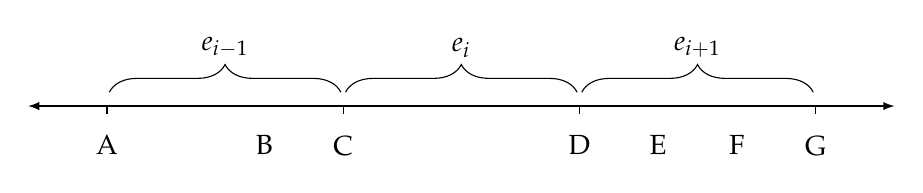
\begin{tikzpicture}
% axis
\draw[latex-latex] (0,0) -- (11,0) ;

% epoch braces
\draw [decorate,decoration={brace,amplitude=10pt} ,yshift=5pt] (1.03,0) -- (3.97,0)
  node [midway, above, yshift=9pt]{$e_{i-1}$};
\draw [decorate,decoration={brace,amplitude=10pt} ,yshift=5pt] (4.03,0) -- (6.97,0)
  node [midway, above, yshift=9pt]{$e_{i}$};
\draw [decorate,decoration={brace,amplitude=10pt} ,yshift=5pt] (7.03,0) -- (9.97,0)
  node [midway, above, yshift=9pt]{$e_{i+1}$};

% epoch boundaries
\foreach \x in  {1,4,7,10}
  \draw[shift={(\x,0)}] (0pt,0pt) -- (0pt,-3pt);

\node at (1,-0.5) {A};
\node at (3,-0.5) {B};
\node at (4,-0.5) {C};
\node at (7,-0.5) {D};
\node at (8,-0.5) {E};
\node at (9,-0.5) {F};
\node at (10,-0.5) {G};

\end{tikzpicture}

We must therefore store the last three stake distributions.
The mnemonic ``mark, set, go'' will be used to keep
track of the snapshots, where the label ``mark'' refers to the most recent snapshot,
and ``go'' refers to the snapshot that is ready to be used in the reward calculation.
In the above diagram, the snapshot taken at (A) is labeled ``mark'' during epoch $e_{i-1}$,
``set'' during epoch $e_i$ and ``go'' during epoch $e_{i+1}$. At (G) the snapshot
taken at (A) is no longer needed and will be discarded.

The two main transition systems in this section are:
\begin{itemize}
  \item The transition system named $\mathsf{EPOCH}$, which is defined in
    Section~\ref{sec:total-epoch}, covers what happens at the epoch boundary,
    such as at (A), (C), (D) and (G).
  \item The transition named $\mathsf{RUPD}$, which is defined in
    Section~\ref{sec:reward-update-trans}, covers the reward calculation that
    happens between (E) and (F).
\end{itemize}


\begin{note}
  Between time D and E we are concerned with chain growth and stability.
  Therefore this duration can be stated as 2k blocks (to state it in slots requires details about
  the particular version of the Ouroboros protocol). The duration between F and G is also 2k blocks.
  Between E and F a single honest block is enough to ensure a random nonce.
\end{note}

\subsection{Example Illustration of the Reward Cycle}
\label{sec:illustration-reward-cycle}

\definecolor{epochColor}{rgb} {1.00,0.50,0.00}
\definecolor{aliceColor}{rgb} {0.65,0.00,0.00}
\definecolor{bobColor}{rgb} {0.00,0.50,0.00}
\definecolor{bob2Color}{rgb} {0.00,0.95,0.00}
\definecolor{snapshot1}{rgb} {0.00,0.00,0.90}
\definecolor{snapshot2}{rgb} {0.00,0.60,0.90}

\begin{tikzpicture}

  % Axis
  \draw [thick] (-0.2,0) -- (13,0);
  \draw (0,-.2) -- (0, .2);
  \draw (3,-.2) -- (3, .2);
  \draw (6,-.2) -- (6, .2);
  \draw (9,-.2) -- (9, .2);
  \draw (12,-.2) -- (12, .2);
  \node[align=center, below, color=epochColor] at (1.5,0.5)
    {$e_1$};
  \node[align=center, below, color=epochColor] at (4.5,0.5)
    {$e_2$};
  \node[align=center, below, color=epochColor] at (7.5,0.5)
    {$e_3$};
  \node[align=center, below, color=epochColor] at (10.5,0.5)
    {$e_4$};

  % Alice
  % Alice's circle
  \draw [aliceColor, fill] (0,3) circle [radius=0.5];
  \node [white] at (0,3) {Alice};
  % Alice's delegation line
  \draw [->,thick, aliceColor] (0.4,2.65) to (2,0.05);
  \node [aliceColor] at (2.2,2) {delegate to Bob};

  % Bob
  % Bob's circle
  \draw [bobColor, fill] (0,-3) circle [radius=0.5];
  \node [white] at (0,-3) {Bob};
  % Bob's registration line
  \draw [->,thick, bobColor] (0.2,-2.50) to (1,-0.05);
  \node [align=left, below, bobColor] at (-0.5,-0.5) {initial pool \\ registration};
  % Bob's re-registration line
  \draw [->,thick, bob2Color] (0.45,-2.65) to (2.90,-0.05);
  \node [bob2Color] at (2,-2.8) {re-registration};
  % Bob's cached parameter change
  \draw [->,thick, bob2Color] (2.9,-0.2) to [out=280, in=180] (3,-2)
     to [out=0, in=290] (3.1,-0.2);

  % Alice time to re-delegate
  \draw [decorate, decoration = {brace, mirror, amplitude=10pt}, aliceColor, thick]
    (3.2,-0.2) to (5.9,-0.2);
  \node [align=center, below, aliceColor] at (5.1,-0.5)
    {Alice's opportunity \\ to re-delegate \\ before Bob's new \\ parameters};

  % Bob's blocks
  % epoch e3
  \draw [fill=bobColor,bobColor] (6.3,-.1) rectangle (6.5,-.3);
  \draw [fill=bobColor,bobColor] (6.7,-.1) rectangle (6.9,-.3);
  \draw [fill=bobColor,bobColor] (7.4,-.1) rectangle (7.6,-.3);
  \draw [fill=bobColor,bobColor] (8.4,-.1) rectangle (8.6,-.3);
  \draw [decorate, decoration = {brace, mirror, amplitude=10pt}, bobColor, thick]
    (6.2, -0.4) to (8.9,-0.4);
  \draw [->,thick, bobColor] (7.6, -0.8) to [out=315,in=200] (8.4, -1.2)
     to [] (9.6, -0.9);

  % epoch e4
  \draw [fill=bob2Color,bob2Color] (9.9,-.1) rectangle (10.1,-.3);
  \draw [fill=bob2Color,bob2Color] (10.4,-.1) rectangle (10.6,-.3);
  \draw [fill=bob2Color,bob2Color] (10.8,-.1) rectangle (11.0,-.3);
  \draw [decorate, decoration = {brace, mirror, amplitude=10pt}, bob2Color, thick]
    (9.7, -0.4) to (11.2,-0.4);
  \draw [->,thick, bob2Color] (10.6, -0.8) to [out=315,in=200] (11.4, -1.2)
     to [] (12.6, -0.9);

  % Snapshots
  \draw [->,thick, snapshot1] (3,0.3) to [out=90,in=150] (9,0.5)
     to [out=330,in=180] (10,-1) to [out=0,in=-135] (12,0) ;
   \node [snapshot1] at (2.7,1.2) {mark};
   \node [snapshot1] at (6,1.9) {set};
   \node [snapshot1] at (9,0.9) {go};

  \draw [->,thick, snapshot2] (6,0.3) to [out=90,in=150] (12,0.5)
     to [out=330,in=180] (13,-1);
   \node [snapshot2] at (5.7,1.2) {mark};
   \node [snapshot2] at (9,1.9) {set};
   \node [snapshot2] at (12,0.9) {go};
\end{tikzpicture}

Bob registers his stake pool in epoch $e_1$.
Alice delegates to Bob's stake pool in epoch $e_1$.
Just before the end of epoch $e_1$, Bob submits a stake pool re-registration,
changing his pool parameters. The change in parameters is not immediate,
as shown by the curved arrow around the epoch boundary.

A snapshot is taken on the $e_1$/$e_2$ boundary. It is labeled ``mark'' initially.
This snapshot includes Alice's delegation to Bob's pool, and Bob's pool parameters
and listed in the initial pool registration certificate.

If Alice changes her delegation choice any time during epoch $e_2$,
she will never be effected by Bob's change of parameters.

A new snapshot is taken on the $e_2$/$e_3$ boundary.
The previous (darker blue) snapshot is now labeled ``set'', and the new one labeled ``mark''.
The ``set'' snapshot is used for leader election in epoch $e_3$.

On the $e_3$/$e_4$ boundary, the darker blue snapshot is labeled ``go'' and
the lighter blue snapshot is labeled ``set''.
Bob's stake pool performance during epoch $e_3$ (he produced 4 blocks)
will be used with the darker blue snapshot for the rewards which will
be handed out at the beginning of epoch $e_5$.

\subsection{Helper Functions and Accounting Fields}
\label{sec:stake-dist-helpers}

Figure~\ref{fig:funcs:epoch-helper-rewards} defines four helper functions needed
throughout the rest of the section.

\begin{itemize}
  \item The function $\fun{obligation}$ calculates the the minimal amount of coin needed to
    pay out all deposit refunds.
  \item The function $\fun{poolStake}$ filters the stake distribution to one stake pool.
\end{itemize}


%%
%% Figure - Helper Functions for Epoch Rules
%%
\begin{figure}[htb]
  \emph{Total possible refunds}
  \begin{align*}
    & \fun{obligation} \in \PParams \to (\StakeCredential \mapsto \Coin)
    \to (\KeyHash_{pool}\mapsto\PoolParam) \to \Coin \\
    & \obligation{pp}{rewards}{poolParams} = \\
    & ~~~~~
    (\fun{keyDeposit}~\var{pp}) \cdot|\var{rewards}| +
    (\fun{poolDeposit}~\var{pp}) \cdot|\var{poolParams}| \\
  \end{align*}
  %
  \emph{Filter Stake to one Pool}
  \begin{align*}
      & \fun{poolStake} \in \KeyHash_{pool} \to (\KeyHash_{stake} \mapsto \KeyHash_{pool})
        \to \Stake \to \Stake \\
      & \poolStake{hk}{delegs}{stake} =
        \dom{(\var{delegs}\restrictrange\{hk\})\restrictdom\var{stake}}
  \end{align*}

  \caption{Helper Functions used in Rewards and Epoch Boundary}
  \label{fig:funcs:epoch-helper-rewards}
\end{figure}


The Figure~\ref{fig:defs:accounting} lists the accounting fields, denoted by $\Acnt$,
which will be used throughout this section. It consists of:
\begin{itemize}
  \item The value $\var{treasury}$ tracks the amount of coin currently stored in the treasury.
    Initially there will be no way to remove these funds.
  \item The value $\var{reserves}$ tracks the amount of coin currently stored in the reserves.
    This pot is used to pay rewards.
\end{itemize}
More will be said about the general accounting system in Section~\ref{sec:reward-calc}.

%%
%% Figure - Accounting fields
%%
\begin{figure}[htb]
  \emph{Accounting Fields}
  \begin{equation*}
    \Acnt =
    \left(
      \begin{array}{r@{~\in~}ll}
        \var{treasury} & \Coin & \text{treasury pot}\\
        \var{reserves} & \Coin & \text{reserve pot}\\
      \end{array}
    \right)
  \end{equation*}
  %
  \caption{Accounting fields}
  \label{fig:defs:accounting}
\end{figure}


\subsection{Stake Distribution Calculation}
\label{sec:stake-dist-calc}

This section defines the stake distribution calculations.
Figure~\ref{fig:epoch-defs} introduces three new derived types:
\begin{itemize}
  \item $\type{BlocksMade}$ represents the number of blocks each stake pool produced
    during an epoch.
  \item $\type{Stake}$ represents the amount of stake (in $\type{Coin}$) controlled by each
    stake pool.
\end{itemize}

%%
%% Figure - Epoch Abstract Types
%%
\begin{figure}[htb]
  \emph{Derived types}
  %
  \begin{equation*}
    \begin{array}{r@{~\in~}l@{\qquad=\qquad}lr}
      \var{blocks}
      & \BlocksMade
      & \KeyHash_{pool} \mapsto \N
      & \text{blocks made by stake pools} \\
      \var{stake}
      & \Stake
      & \Credential \mapsto \Coin
      & \text{stake} \\
    \end{array}
  \end{equation*}
  \caption{Epoch definitions}
  \label{fig:epoch-defs}
\end{figure}

The stake distribution calculation is given in Figure~\ref{fig:functions:stake-distribution}.

\begin{itemize}
\item $\fun{aggregate_{+}}$ takes a relation on $A\times B$, where $B$ is any
  monoid $(B,+,e)$ and returns a map from each $a\in A$ to the ``sum'' (using
  the monoidal $+$ operation) of all $b\in B$ such that $(a, b)\in A\times B$.
\item $\fun{stakeDistr}$ uses the $\fun{aggregate_{+}}$ function and several relations to
    compute the stake distribution, mapping each hashkey to the total coin under its control.
    Keys that are not both registered and delegated are filtered out.
    The relation passed to $\fun{aggregate_{+}}$ is made up of:
    \begin{itemize}
      \item $\fun{stakeCred_b}^{-1}$, relating credentials to (base) addresses
      \item $\left(\fun{addrPtr}\circ\var{ptr}\right)^{-1}$, relating credentials to (pointer)
        addresses
      \item $\range{utxo}$, relating addresses to coins
      \item $\fun{stakeCred_r}^{-1}\circ\var{rewards}$, relating (reward) addresses to coins
    \end{itemize}
    The notation for relations is explained in Section~\ref{sec:notation-shelley}.
\end{itemize}

%%
%% Figure Functions for Stake Distribution
%%
\begin{figure}[htb]
  \emph{Aggregation (for a monoid B)}
  %
  \begin{align*}
      & \fun{aggregate_{+}} \in \powerset{(A \times B)} \to (A\mapsto B) \\
      & \fun{aggregate_{+}}~\var{R} = \left\{a\mapsto \sum_{(a,b)\in\var{R}}b
          ~\mid~a\in\dom\var{R}\right\} \\
  \end{align*}
  %
  \emph{Stake Distribution (using functions and maps as relations)}
  %
  \begin{align*}
      & \fun{stakeDistr} \in \UTxO \to \DState \to \PState \to \Snapshot \\
      & \fun{stakeDistr}~{utxo}~{dstate}~{pstate} = \\
      & ~~~~ \big((\dom{\var{activeDelegs}})
      \restrictdom\left(\fun{aggregate_{+}}~\var{stakeRelation}\right),
    ~\var{delegations},~\var{poolParams}\big)\\
      & \where \\
      & ~~~~ (~\var{rewards},~\var{delegations},~\var{ptrs},~\wcard,~\wcard,~\wcard)
        = \var{dstate} \\
      & ~~~~ (~\var{poolParams},~\wcard,~\wcard) = \var{pstate} \\
      & ~~~~ \var{stakeRelation} = \left(
        \left(\fun{stakeCred_b}^{-1}\cup\left(\fun{addrPtr}\circ\var{ptr}\right)^{-1}\right)
        \circ\left(\range{\var{utxo}}\right)
        \right)
        \cup \var{rewards} \\
      & ~~~~ \var{activeDelegs} =
               (\dom{rewards}) \restrictdom \var{delegations} \restrictrange (\dom{poolParams}) \\
  \end{align*}

  \caption{Stake Distribution Function}
  \label{fig:functions:stake-distribution}
\end{figure}

\clearpage

\subsection{Snapshot Transition}
\label{sec:snapshots}

The state transition types for stake distribution snapshots are given in
Figure~\ref{fig:ts-types:snapshot}.
Each snapshot consists of:
\begin{itemize}
  \item $\var{stake}$, a stake distribution, which is defined in
    Figure~\ref{fig:epoch-defs} as a mapping of credentials to coin.
  \item $\var{delegations}$, a delegation map, mapping credentials to stake pools.
  \item $\var{poolParameters}$, storing the pool parameters of each stake pool.
\end{itemize}

The type $\type{\Snapshots}$ contains the
information needing to be saved on the epoch boundary:
\begin{itemize}
  \item $\var{pstake_{mark}}$, $\var{pstake_{set}}$ and $\var{pstake_{go}}$ are the three
    snapshots as explained in Section~\ref{sec:reward-overview}.
  \item $\var{feeSS}$ stores the fees which are added to the reward pot during
    the next reward update calculation, which is then subtracted from the fee pot
    on the epoch boundary.
\end{itemize}

%%
%% Figure - Snapshots Defs
%%
\begin{figure}[htb]
  \emph{Snapshots}
  \begin{equation*}
    \Snapshot =
    \left(
      \begin{array}{r@{~\in~}ll}
        \var{stake} & \Stake & \text{stake distribution}\\
        \var{delegations} & \Credential\mapsto\KeyHash_{pool}
                          & \text{stake delegations}\\
        \var{poolParameters} & \KeyHash_{pool} \mapsto \PoolParam & \text{pool parameters }\\
      \end{array}
    \right)
  \end{equation*}

  \begin{equation*}
    \Snapshots =
    \left(
      \begin{array}{r@{~\in~}ll}
        \var{pstake_{mark}} & \Snapshot & \text{newest stake}\\
        \var{pstake_{set}}  & \Snapshot & \text{middle stake}\\
        \var{pstake_{go}}   & \Snapshot & \text{oldest stake}\\
        \var{feeSS} & \Coin & \text{fee snapshot}\\
      \end{array}
    \right)
  \end{equation*}
  %
  \emph{Snapshot transitions}
  \begin{equation*}
    \_ \vdash
    \var{\_} \trans{snap}{} \var{\_}
    \subseteq \powerset (\LState \times \Snapshots \times \Snapshots)
  \end{equation*}
  %
  \caption{Snapshot transition-system types}
  \label{fig:ts-types:snapshot}
\end{figure}

The snapshot transition rule is given in Figure~\ref{fig:rules:snapshot}.
This transition has no preconditions and results in the following state change:

\begin{itemize}
  \item The oldest snapshot is replaced with the penultimate one.
  \item The penultimate snapshot is replaced with the newest one.
  \item The newest snapshot is replaced with one just calculated.
  \item The current fees pot is stored in $\var{feeSS}$. Note that this value will not
    change during the epoch, unlike the $\var{fees}$ value in the UTxO state.
\end{itemize}

%%
%% Figure - Snapshot Rule
%%
\begin{figure}[htb]
  \begin{equation}\label{eq:snapshot}
    \inference[Snapshot]
    {
      {
      \begin{array}{r@{~\leteq~}l}
        ((\var{utxo},~\wcard,\var{fees},~\wcard),~(\var{dstate},~\var{pstate})) & \var{lstate} \\
        \var{stake} & \stakeDistr{utxo}{dstate}{pstate} \\
      \end{array}
      }
    }
    {
      \begin{array}{r}
        \var{lstate} \\
      \end{array}
      \vdash
      \left(
        \begin{array}{r}
          \var{pstake_{mark}}\\
          \var{pstake_{set}}\\
          \var{pstake_{go}}\\
          \var{feeSS} \\
        \end{array}
      \right)
      \trans{snap}{}
      \left(
        \begin{array}{r}
          \varUpdate{\var{stake}} \\
          \varUpdate{\var{pstake_{mark}}} \\
          \varUpdate{\var{pstake_{set}}} \\
          \varUpdate{\var{fees}} \\
        \end{array}
      \right)
    }
  \end{equation}
  \caption{Snapshot Inference Rule}
  \label{fig:rules:snapshot}
\end{figure}

\clearpage

\subsection{Pool Reaping Transition}
\label{sec:pool-reap}

Figure~\ref{fig:ts-types:pool-reap} defines the types for the pool reap transition,
which is responsible for removing pools slated for retirement in the given epoch.

%%
%% Figure - Pool Reap Defs
%%
\begin{figure}[htb]
  \emph{Pool Reap State}
  \begin{equation*}
    \PlReapState =
    \left(
      \begin{array}{r@{~\in~}ll}
        \var{utxoSt} & \UTxOState & \text{utxo state}\\
        \var{acnt} & \Acnt & \text{accounting}\\
        \var{dstate} & \DState & \text{delegation state}\\
        \var{pstate} & \PState & \text{pool state}\\
      \end{array}
    \right)
  \end{equation*}
  %
  \emph{Pool Reap transitions}
  \begin{equation*}
    \_ \vdash \_ \trans{poolreap}{\_} \_ \in
    \powerset (\PParams \times \PlReapState \times \Epoch \times \PlReapState)
  \end{equation*}
  %
  \caption{Pool Reap Transition}
  \label{fig:ts-types:pool-reap}
\end{figure}


The pool-reap transition rule is given in Figure~\ref{fig:rules:pool-reap}.
This transition has no preconditions and results in the following state change:

\begin{itemize}
  \item For each retiring pool, the refund for the pool registration deposit is added to the
    pool's registered reward account, provided the reward account is still registered.
  \item The sum of all the refunds attached to unregistered reward accounts are added to the
    treasury.
  \item The deposit pool is reduced by the amount of claimed and unclaimed refunds.
  \item Any delegation to a retiring pool is removed.
  \item Each retiring pool is removed from all four maps in the pool state.
\end{itemize}

%%
%% Figure - Pool Reap Rule
%%
\begin{figure}[htb]
  \begin{equation}\label{eq:pool-reap}
    \inference[Pool-Reap]
    {
      {
      \begin{array}{r@{~\leteq~}l}
        \var{retired} & \dom{(\var{retiring}^{-1}~\var{e})} \\
        \var{pr} & \left\{
                   \var{hk}\mapsto(\fun{poolDeposit}~\var{pp})
                     \mid
                     \var{hk}\in\var{retired}
                   \right\}\\
        \var{rewardAcnts}
                 & \{\var{hk}\mapsto \fun{poolRAcnt}~\var{pool} \mid
                   \var{hk}\mapsto\var{pool} \in \var{retired}\restrictdom\var{poolParams} \} \\
        \var{rewardAcnts'} & \left\{
                               \sum\limits_{\wcard\mapsto c\in\var{pr}\circ\var{rewardAcnts}^{-1}(a)} c
                               \mathrel{\Bigg|}
			       a\in\range{rewardAcnts}
                             \right\} \\
        \var{refunds} & \dom{rewards}\restrictdom\var{rewardAcnts'} \\
        \var{mRefunds} & \dom{rewards}\subtractdom\var{rewardAcnts'} \\
        \var{refunded} & \sum\limits_{\wcard\mapsto c\in\var{refunds}} c \\
        \var{unclaimed} & \sum\limits_{\wcard\mapsto c\in\var{mRefunds}} c \\
      \end{array}
      }
    }
    {
      \var{pp}
      \vdash
      \left(
        \begin{array}{r}
          \var{utxo} \\
          \var{deposited} \\
          \var{fees} \\
          \var{ppup} \\
          ~ \\
          \var{treasury} \\
          \var{reserves} \\
          ~ \\
          \var{rewards} \\
          \var{delegations} \\
          \var{ptrs} \\
          \var{genDelegs} \\
          \var{fGenDelegs} \\
          \var{i_{rwd}} \\
          ~ \\
          \var{poolParams} \\
          \var{fPoolParams} \\
          \var{retiring} \\
        \end{array}
      \right)
      \trans{poolreap}{e}
      \left(
        \begin{array}{rcl}
          \var{utxo} \\
          \varUpdate{\var{deposited}}
          & \varUpdate{-}
          & \varUpdate{(\var{unclaimed} + \var{refunded})} \\
          \var{fees} \\
          \var{ppup} \\
          ~ \\
          \varUpdate{\var{treasury}} & \varUpdate{+} & \varUpdate{\var{unclaimed}} \\
          \var{reserves} \\
          ~ \\
          \varUpdate{\var{rewards}} & \varUpdate{\unionoverridePlus} & \varUpdate{\var{refunds}} \\
          \varUpdate{\var{delegations}} & \varUpdate{\subtractrange} & \varUpdate{\var{retired}} \\
          \var{ptrs} \\
          \var{genDelegs} \\
          \var{fGenDelegs} \\
          \var{i_{rwd}}\\
          ~ \\
          \varUpdate{\var{retired}} & \varUpdate{\subtractdom} & \varUpdate{\var{poolParams}} \\
          \varUpdate{\var{retired}} & \varUpdate{\subtractdom} & \varUpdate{\var{fPoolParams}} \\
          \varUpdate{\var{retired}} & \varUpdate{\subtractdom} & \varUpdate{\var{retiring}} \\
        \end{array}
      \right)
    }
  \end{equation}
  \caption{Pool Reap Inference Rule}
  \label{fig:rules:pool-reap}
\end{figure}

\clearpage

\subsection{Protocol Parameters Update Transition}
\label{sec:pparam-update}

Finally, reaching the epoch boundary may trigger a change in the protocol parameters.
The protocol parameters environment consists of the delegation and pool states,
and the signal is an optional new collection of protocol parameters
The state change is a change of the $\UTxOState$, the $\Acnt$ states and the current $\PParams$.
The type of this state transition is given in Figure~\ref{fig:ts-types:new-proto-param}.

%%
%% Figure - New Proto Param Defs
%%
\begin{figure}[htb]
  \emph{New Proto Param environment}
  \begin{equation*}
    \NewPParamEnv =
    \left(
      \begin{array}{r@{~\in~}ll}
        \var{dstate} & \DState & \text{delegation state}\\
        \var{pstate} & \PState & \text{pool state}\\
      \end{array}
    \right)
  \end{equation*}
  %
  \emph{New Proto Param States}
  \begin{equation*}
    \NewPParamState =
    \left(
      \begin{array}{r@{~\in~}ll}
        \var{utxoSt} & \UTxOState & \text{utxo state}\\
        \var{acnt} & \Acnt & \text{accounting}\\
        \var{pp} & \PParams & \text{current protocol parameters}\\
      \end{array}
    \right)
  \end{equation*}
  %
  \emph{New Proto Param transitions}
  \begin{equation*}
    \_ \vdash
    \var{\_} \trans{newpp}{\_} \var{\_}
    \subseteq \powerset (\NewPParamEnv \times \NewPParamState \times \PParams^? \times \NewPParamState)
  \end{equation*}
  %
  \caption{New Proto Param transition-system types}
  \label{fig:ts-types:new-proto-param}
  %
  \emph{Helper Functions}
  \begin{align*}
      & \fun{updatePpup} \in \UTxOState \to \PParams \to \UTxOState\\
      & \fun{updatePpup}~\var{utxoSt}~\var{pp} =
      \begin{cases}
        (\var{utxo},\var{deposited},\var{fees},(\var{fpup},~\emptyset))
        &
        \var{canFollow}
        \\
        (\var{utxo},\var{deposited},\var{fees},(\emptyset,~\emptyset))
        &
        \text{otherwise} \\
      \end{cases}\\
      & ~~~\where \\
      & ~~~~~~~\var{canFollow} =
        \forall\var{ps}\in\range{pup},~
        \var{pv}\mapsto\var{v}\in\var{ps}\implies\fun{pvCanFollow}~(\fun{pv}~\var{pp})~\var{v}
        \\
      & ~~~~~~~(\var{utxo},\var{deposited},\var{fees},(\var{pup},~\var{fpup})) = \var{utxoSt} \\
  \end{align*}
\end{figure}


Figure~\ref{fig:rules:new-proto-param} defines the new protocol parameter transition.
The transition has two rules, depending on whether or not the new protocol parameters
meet some requirements.
In particular, we require that the new parameters would not incur a debt of the system that
can not be covered by the reserves, and that the max block size is greater than the sum of the
max transaction size and the max header size.
If the requirements are met, the new protocol parameters are accepted, the proposal is reset,
and the reserves are adjusted to account for changes in the deposits.
Otherwise, the only change is that the proposal is reset.

The $\mathsf{NEWPP}$ rule also cleans up the protocol parameter update proposals,
by calling $\fun{updatePpup}$ on the UTxO state.
The $\fun{updatePpup}$ sets the protocol parameter updates to the future protocol
parameter updates provided the protocol versions all can follow from the
version given in the protocol parameters, or the emptyset otherwise.
In any case, the future protocol parameters update proposals are set to the empty set.
If new protocol parameters are being adopted, then these is the value given to
$\fun{updatePpup}$, otherwise the old parameters are given.

Regarding adjusting the reserves for changes in the deposits, one of three things happens:

\begin{itemize}
  \item If the new protocol parameters mean that \textbf{fewer} funds are required in the
    deposit pot to cover all possible refunds, then the excess is moved to the reserves.

  \item If the new protocol parameters mean that \textbf{more} funds are required in the
    deposit pot to cover all possible refunds and the difference is \textbf{less} than
    the reserve pot, then funds are moved from the reserve pot to cover the difference.

  \item If the new protocol parameters mean that \textbf{more} funds are required in the
    deposit pot to cover all possible refunds and the difference is \textbf{more} than
    the reserve pot, then Rule~\ref{eq:new-pc-denied} meets the precondition and the
    only change of state is that the update proposals are reset.
\end{itemize}

Note that here, unlike most of the inference rules in this document,
the $\var{utxoSt'}$ and the $\var{acnt'}$ do not come from valid UTxO or
accounts transitions in the antecedent. We simply define the consequent
transition using these directly (instead of listing all the fields in both
states in the consequent transition). It is done this way here
for ease of reading.

%%
%% Figure - New Proto Param Rule
%%
\begin{figure}[htb]
  \begin{equation}\label{eq:new-pc-accepted}
    \hspace{-0.3cm}
    \inference[New-Proto-Param-Accept]
    {
      \var{pp_{new}}\neq\Nothing \\~\\
      {\begin{array}{rcl}
         (\var{utxo},~\var{deposited},~\var{fees},~\var{ppup}) & \leteq & \var{utxoSt} \\
         \var{(\var{rewards},~\wcard,~\wcard,~\wcard,~\wcard,~\var{i_{rwd}})} &
         \leteq & \var{dstate}\\
         \var{(\var{poolParams},~\wcard,~\wcard)} & \leteq & \var{pstate}\\
         \var{oblg_{cur}} & \leteq & \obligation{pp}{rewards}{poolParams} \\
         \var{oblg_{new}} & \leteq & \obligation{pp_{new}}{rewards}{poolParams} \\
         \var{diff} & \leteq & \var{oblg_{cur}} - \var{oblg_{new}}\\
      \end{array}}
      \\~\\~\\
      \var{oblg_{cur}} = \var{deposited} \\
      \var{reserves} + \var{diff} \geq \sum\limits_{\wcard\mapsto\var{val}\in\var{i_{rwd}}} val \\
      \fun{maxTxSize}~\var{pp_{new}} + \fun{maxHeaderSize}~\var{pp_{new}} <
        \fun{maxBlockSize}~\var{pp_{new}}
      \\~\\
        \var{utxoSt'} \leteq
        \left(\var{utxo},~\varUpdate{oblg_{new}},~\var{fees},~\var{ppup}\right)
      \\
      \var{utxoSt''} \leteq \fun{updatePpup}~\var{utxoSt'}~\var{pp_{new}}
      \\~\\
      (\var{treasury},~\var{reserves})\leteq \var{acnt} \\
      \var{acnt'} \leteq (\var{treasury},~\varUpdate{reserves + diff}) \\
    }
    {
      \begin{array}{l}
        \var{dstate}\\
        \var{pstate}\\
      \end{array}
      \vdash
      \left(
        \begin{array}{r}
          \var{utxoSt} \\
          \var{acnt} \\
          \var{pp}
        \end{array}
      \right)
      \trans{newpp}{\var{pp_{new}}}
      \left(
        \begin{array}{rcl}
          \varUpdate{utxoSt''}\\
          \varUpdate{acnt'} \\
          \varUpdate{\var{pp_{new}}} \\
        \end{array}
      \right)
    }
  \end{equation}

  \nextdef

  \begin{equation}\label{eq:new-pc-denied}
    \inference[New-Proto-Param-Denied]
    {
      \left({\begin{array}{c}
            \var{pp_{new}}=\Nothing \\
        \lor \\
        \var{reserves} + \var{diff} < \sum\limits_{\wcard\mapsto\var{val}\in\var{i_{rwd}}} val\\
        \lor \\
        \fun{maxTxSize}~\var{pp_{new}} + \fun{maxHeaderSize}~\var{pp_{new}} \geq
          \fun{maxBlockSize}~\var{pp_{new}}
      \end{array}}\right)
      \\~\\~\\
      {\begin{array}{rcl}
          \var{(\var{rewards},~\wcard,~\wcard,~\wcard,~\wcard,~\var{i_{rwd}})} &
          \leteq & \var{dstate}\\
         \var{(\var{poolParams},~\wcard,~\wcard)} & \leteq & \var{pstate}\\
          \var{oblg_{cur}} & \leteq & \obligation{pp}{rewards}{poolParams} \\
          \var{oblg_{new}} & \leteq & \obligation{pp_{new}}{rewards}{poolParams} \\
         \var{diff} & \leteq & \var{oblg_{cur}} - \var{oblg_{new}}
      \end{array}}
      \\~\\~\\
      \var{utxoSt'} \leteq \fun{updatePpup}~\var{utxoSt}~\var{pp} \\
    }
    {
      \begin{array}{l}
        \var{dstate}\\
        \var{pstate}\\
      \end{array}
      \vdash
      \left(
        \begin{array}{r}
          \var{utxoSt} \\
          \var{acnt} \\
          \var{pp}
        \end{array}
      \right)
      \trans{newpp}{\var{pp_{new}}}
      \left(
        \begin{array}{rcl}
          \varUpdate{utxoSt'}\\
          \var{acnt} \\
          \var{pp}
        \end{array}
      \right)
    }
  \end{equation}
  \caption{New Proto Param Inference Rule}
  \label{fig:rules:new-proto-param}
\end{figure}

\clearpage

\subsection{Complete Epoch Boundary Transition}
\label{sec:total-epoch}

Finally, it is possible to define the complete epoch boundary transition type,
which is defined in Figure~\ref{fig:ts-types:epoch}.
The transition has no evironment.
The state is made up of the the accounting state, the snapshots, the ledger state and the
protocol parameters.
The transition uses a helper function $\fun{votedValue}$ which returns
the consensus value of update proposals in the event that consensus is met.
\textbf{Note that} $\fun{votedValue}$
\textbf{is only well-defined if } $\var{quorum}$
\textbf{is greater than half the number of core nodes, i.e.}
$\Quorum > |\var{genDelegs}|/2$ \textbf{.}

%%
%% Figure - Epoch Defs
%%
\begin{figure}[htb]
  \emph{Epoch States}
  \begin{equation*}
    \EpochState =
    \left(
      \begin{array}{r@{~\in~}ll}
        \var{acnt} & \Acnt & \text{accounting}\\
        \var{ss} & \Snapshots & \text{snapshots}\\
        \var{ls} & \LState & \text{ledger state}\\
        \var{prevPp} & \PParams & \text{previous protocol parameters}\\
        \var{pp} & \PParams & \text{protocol parameters}\\
      \end{array}
    \right)
  \end{equation*}
  %
  \emph{Epoch transitions}
  \begin{equation*}
    \vdash
    \var{\_} \trans{epoch}{\_} \var{\_}
    \subseteq \powerset (\EpochState \times \Epoch \times \EpochState)
  \end{equation*}
  %
  \emph{Accessor Functions}
  \begin{equation*}
    \begin{array}{r@{~\in~}lr}
      \fun{getIR} & \EpochState \to (\StakeCredential \mapsto \Coin)
                  & \text{get instantaneous rewards} \\
    \end{array}
  \end{equation*}
  %
  \emph{Helper Functions}
  \begin{align*}
      & \fun{votedValue} \in (\KeyHashGen\mapsto\PParamsUpdate) \to \PParams \to \N \to \PParamsUpdate^?\\
      & \fun{votedValue}~\var{pup}~\var{pp}~\var{quorum} =
      \begin{cases}
        \var{pp}\unionoverrideRight\var{p}
          & \exists! p\in\range{pup}~(|pup\restrictrange p|\geq \var{quorum}) \\
        \Nothing & \text{otherwise} \\
      \end{cases}
  \end{align*}
  %
  \caption{Epoch transition-system types}
  \label{fig:ts-types:epoch}
\end{figure}


The epoch transition rule calls $\mathsf{SNAP}$, $\mathsf{POOLREAP}$ and $\mathsf{NEWPP}$
in sequence. It also stores the previous protocol parameters in $\var{prevPp}$.
The previous protocol parameters will be used for the reward calculation in the upcoming epoch,
note that they correspond to the epoch for which the rewards are being calculated.
Additionally, this transition also adopts the pool parameters $\var{fPoolParams}$
corresponding to the pool re-registration certificates which we submitted late in the ending epoch.
The ordering of these rules is important.
The stake pools which will be updated by $\var{fPoolParams}$ or
reaped during the $\mathsf{POOLREAP}$ transition must still be a
part of the new snapshot, and so $\mathsf{SNAP}$ must occur before these two actions.
Moreover, $\mathsf{SNAP}$ sets the deposit pot equal to current obligation,
which is a property that is preserved by $\mathsf{POOLREAP}$ and which
is necessary for the preservation of Ada property in the $ \mathsf{NEWPP}$ transition.

%%
%% Figure - Epoch Rule
%%
\begin{figure}[htb]
  \begin{equation}\label{eq:epoch}
    \inference[Epoch]
    {
      {
        \begin{array}{r}
          \var{lstate} \\
        \end{array}
      }
      \vdash
      { \var{ss} }
      \trans{\hyperref[fig:rules:snapshot]{snap}}{}
      { \var{ss'} }
      \\~\\
      (\var{utxoSt},~(\var{dstate},~\var{pstate}))\leteq\var{ls} \\
      (\var{poolParams},~\var{fPoolParams},~\var{retiring})\leteq\var{pstate}
      \\
      \var{pstate'}\leteq(\var{poolParams}\unionoverrideRight\var{fPoolParams},
      ~\emptyset,~\var{retiring})
      \\~\\~\\
      \var{pp}
      \vdash
      \left(
        {
          \begin{array}{r}
            \var{utxoSt} \\
            \var{acnt} \\
            \var{dstate} \\
            \var{pstate'} \\
          \end{array}
        }
      \right)
      \trans{\hyperref[fig:rules:pool-reap]{poolreap}}{e}
      \left(
      {
        \begin{array}{rcl}
            \var{utxoSt'} \\
            \var{acnt'} \\
            \var{dstate'} \\
            \var{pstate''} \\
        \end{array}
      }
      \right)
      \\~\\~\\
      \var{(\wcard,~\wcard,~\wcard,~(\var{pup},\wcard))}\leteq\var{utxoSt'}\\
      \var{pp_{new}}\leteq\fun{votedValue}~\var{pup}~\var{pp}~\Quorum\\
      {
        \begin{array}{r}
          \var{dstate'}\\
          \var{pstate''}\\
        \end{array}
      }
      \vdash
      \left(
        {
          \begin{array}{r}
            \var{utxoSt'} \\
            \var{acnt'} \\
            \var{pp}\\
          \end{array}
        }
      \right)
      \trans{\hyperref[fig:rules:new-proto-param]{newpp}}{\var{pp_{new}}}
      \left(
      {
        \begin{array}{rcl}
            \var{utxoSt''} \\
            \var{acnt''} \\
            \var{pp'}\\
        \end{array}
      }
      \right)
      \\~\\~\\
      \var{ls}' \leteq (\var{utxoSt}'',~(\var{dstate}',~\var{pstate}''))
    }
    {
      \vdash
      \left(
      \begin{array}{r}
        \var{acnt} \\
        \var{ss} \\
        \var{ls} \\
        \var{prevPp} \\
        \var{pp} \\
      \end{array}
      \right)
      \trans{epoch}{e}
      \left(
      \begin{array}{rcl}
        \varUpdate{\var{acnt''}} \\
        \varUpdate{\var{ss'}} \\
        \varUpdate{\var{ls'}} \\
        \varUpdate{\var{pp}} \\
        \varUpdate{\var{pp'}} \\
      \end{array}
      \right)
    }
  \end{equation}
  \caption{Epoch Inference Rule}
  \label{fig:rules:epoch}
\end{figure}

\clearpage

\subsection{Rewards Distribution Calculation}
\label{sec:reward-dist}

This section defines the reward calculation for the proof of stake leader election.
Figure~\ref{fig:functions:rewards} defines the pool reward as described in section
5.5.2 of~\cite{delegation_design}.

\begin{itemize}
  \item The function $\fun{maxPool}$ gives the maximum reward a stake pool can receive in an epoch.
    This is a fraction of the total available rewards for the epoch.
    The result depends on the pool's relative stake, the pool's pledge and the following
    protocol parameters:
    \begin{itemize}
      \item $\var{a_0}$, the leader-stake influence
      \item $n_{opt}$, the optimal number of saturated stake pools
    \end{itemize}
  \item The function $\fun{mkApparentPerformance}$ computes the apparent performance of a stake pool.
    It depends on the protocol parameter $d$, the relative stake $\sigma$, the number $n$ of blocks
    the pool added to the chain and the total number $\overline{N}$ of blocks added to the chain in
    the last epoch.

\end{itemize}

%%
%% Figure - Functions for the Reward Calculation
%%
\begin{figure}[htb]
  \emph{Maximal Reward Function, called $f(s,\sigma)$ in section 5.5.2 of~\cite{delegation_design}}
  %
  \begin{align*}
      & \fun{maxPool} \in \PParams \to \Coin \to \unitInterval \to \unitInterval \to \Coin \\
      & \fun{maxPool}~\var{pp}~\var{R}~\sigma~\var{p_r} =
          ~~~\floor*{
             \frac{R}{1 + a_0}
             \cdot
             \left(
               \sigma' + p'\cdot a_0\cdot\frac{\sigma' - p'\frac{z_0-\sigma'}{z_0}}{z_0}
             \right)} \\
      & ~~~\where \\
      & ~~~~~~~a_0 = \fun{influence}~pp \\
      & ~~~~~~~n_{opt} = \fun{nopt}~pp \\
      & ~~~~~~~z_0 = 1/n_{opt} \\
      & ~~~~~~~\sigma'=\min(\sigma,~z_0) \\
      & ~~~~~~~p'=\min(p_r,~z_0) \\
  \end{align*}

  \emph{Apparent Performance, called $\hat{p}$ in section 5.5.2 of~\cite{delegation_design}}
  %
  \begin{align*}
      & \fun{mkApparentPerformance} \in \unitInterval \to \unitInterval \to \N \to \N \to \Q \\
      & \mkApparentPerformance{d}{\sigma}{n}{\overline{N}} =
        \begin{cases}
          \frac{\beta}{\sigma} & \text{if } d < 0.8 \\
          1 & \text{otherwise}
        \end{cases} \\
      & ~~~\where \\
      & ~~~~~~~\beta = \frac{n}{\max(1, \overline{N})} \\
  \end{align*}
  \caption{Functions used in the Reward Calculation}
  \label{fig:functions:rewards}
\end{figure}

\clearpage

Figure~\ref{fig:functions:reward-splitting} gives the calculation for
splitting the pool rewards with its members, as described in 6.5.2 of \cite{delegation_design}.
The portion of rewards allocated to the pool operator and owners is different
than that of the members.

\begin{itemize}
  \item The $\fun{r_{operator}}$ function calculates the leader reward, based on the pool cost,
    margin and the proportion of the pool's total stake.  Note that this reward will go to the
    reward account specified in the pool registration certificate.
  \item The $\fun{r_{member}}$ function calculates the member reward, proportionally to their
    stake after the cost and margin are removed.
\end{itemize}

%%
%% Figure - Functions for the Reward Splitting
%%
\begin{figure}[htb]
  \emph{Pool leader reward, from section 5.5.3 of \cite{delegation_design}}
  %
  \begin{align*}
      & \fun{r_{operator}} \in \Coin \to \PoolParam \to \unitInterval \to \unitIntervalNonNull \to \Coin \\
      & \lReward{\hat{f}}{pool}{s}{\sigma} =
        \begin{cases}
        \hat{f} & \hat{f} \leq c\\
        c + \floor*{(\hat{f} - c)\cdot\left(m + (1-m)\cdot\frac{s}{\sigma}\right) }&
        \text{otherwise.}
      \end{cases} \\
      & ~~~\where \\
      & ~~~~~~~c = \fun{poolCost}~pool \\
      & ~~~~~~~m = \fun{poolMargin}~pool \\
  \end{align*}

  \emph{Pool member reward, from section 5.5.3 of \cite{delegation_design}}
  %
  \begin{align*}
    & \fun{r_{member}} \in \Coin \to \PoolParam \to \unitInterval \to \unitIntervalNonNull \to \Coin \\
    & \mReward{\hat{f}}{pool}{t}{\sigma} =
      \begin{cases}
        0 & \hat{f} \leq c\\
        \floor*{(\hat{f} - c)\cdot(1-m)\cdot\frac{t}{\sigma}} &
        \text{otherwise.}
      \end{cases} \\
    & ~~~\where \\
    & ~~~~~~~c = \fun{poolCost}~pool \\
    & ~~~~~~~m = \fun{poolMargin}~pool \\
  \end{align*}

  \caption{Functions used in the Reward Splitting}
  \label{fig:functions:reward-splitting}
\end{figure}


Finally, the full reward calculation is presented in Figure~\ref{fig:functions:reward-calc}.
The calculation is done pool-by-pool.
\begin{itemize}
\item The $\fun{rewardOnePool}$ function calculates the rewards given out to
  each member of a given pool. The pool leader is identified by the stake
  credential of the pool operator. The function returns the rewards, calculated
  as follows:
    \begin{itemize}
      \item $\var{pstake}$, the total amount of stake controlled by the stake pool.
      \item $\var{ostake}$, the total amount of stake controlled by the stake pool operator
        and owners
      \item $\sigma$, the total proportion of stake controlled by the stake pool.
      \item $\overline{N}$, the expected number of blocks the pool should have produced.
      \item $\var{pledge}$, the pool's pledge in lovelace.
      \item $p_r$, the pool's pledge, as a proportion of active stake.
      \item $\var{maxP}$, maximum rewards the pool can claim if the pledge is met,
        and zero otherwise.
      \item $\var{poolR}$, the pool's actual reward, based on its performance.
      \item $\var{mRewards}$, the member's rewards as a mapping of reward accounts to coin.
      \item $\var{lReward}$, the leader's reward as coin.
      \item $\var{potentialRewards}$, the combination of $\var{mRewards}$ and $\var{lRewards}$.
      \item $\var{rewards}$, the restriction of $\var{potentialRewards}$ to the active
        reward accounts.
    \end{itemize}
  \item The $\fun{reward}$ function applies $\fun{rewardOnePool}$ to each registered stake pool.
\end{itemize}

%%
%% Figure - The Reward Calculation
%%
\begin{figure}[htb]
  \emph{Calculation to reward a single stake pool}
  %
  \begin{align*}
    & \fun{rewardOnePool} \in \PParams \to \Coin \to \N \to \N \to \PoolParam\\
      & ~~~\to \Stake \to \Q \to \Q \to \Coin \to \powerset{\AddrRWD}
           \to (\AddrRWD \mapsto \Coin) \\
      & \fun{rewardOnePool}~\var{pp}~\var{R}~\var{n}~\var{\overline{N}}~\var{pool}~\var{stake}~{\sigma}~{\sigma_a}~\var{tot}~\var{addrs_{rew}} =
          \var{rewards}\\
      & ~~~\where \\
      & ~~~~~~~\var{ostake} = \sum_{\substack{
        hk_\mapsto c\in\var{stake}\\
        hk\in(\fun{poolOwners}~\var{pool})\\
        }} c \\
      & ~~~~~~~\var{pledge} = \fun{poolPledge}~pool \\
      & ~~~~~~~p_{r} = \var{pledge} / \var{tot} \\
      & ~~~~~~~maxP =
      \begin{cases}
        \fun{maxPool}~\var{pp}~\var{R}~\sigma~\var{p_r}&
        \var{pledge} \leq \var{ostake}\\
        0 & \text{otherwise.}
      \end{cases} \\
      & ~~~~~~~\var{appPerf} = \mkApparentPerformance{(\fun{d}~pp)}{\sigma_a}{n}{\overline{N}} \\
      & ~~~~~~~\var{poolR} = \floor{\var{appPerf}\cdot\var{maxP}} \\
      & ~~~~~~~\var{mRewards} = \\
      & ~~~~~~~~~~\left\{
                    \addrRw~hk\mapsto\mReward{poolR}{pool}{\frac{c}{tot}}{\sigma}
                    ~\Big\vert~
                    hk\mapsto c\in\var{stake},~~hk \not\in(\fun{poolOwners}~\var{pool})
                  \right\}\\
      & ~~~~~~~\var{lReward} = \lReward{poolR}{pool}{\frac{\var{ostake}}{tot}}{\sigma} \\
      & ~~~~~~~\var{potentialRewards} =
                 \var{mRewards} \cup
                 \{(\fun{poolRAcnt}~\var{pool})\mapsto\var{lReward}\} \\
      & ~~~~~~~\var{rewards} = \var{addrs_{rew}}\restrictdom{\var{potentialRewards}} \\
  \end{align*}

  \emph{Calculation to reward all stake pools}
  %
  \begin{align*}
      & \fun{reward} \in \PParams \to \BlocksMade \to \Coin\to \powerset{\AddrRWD}
      \to (\KeyHash \mapsto \PoolParam) \\
      & ~~~\to \Stake \to (\KeyHash_{stake} \mapsto \KeyHash_{pool}) \to
      \Coin \to (\AddrRWD \mapsto \Coin)\\
      & \reward{pp}{blocks}{R}{addrs_{rew}}{poolParams}{stake}{delegs}{total}
          = \var{rewards}\\
      & ~~~\where \\
      & ~~~~~~~\var{total}_a = \sum_{\_\mapsto c\in \var{stake}}c \\
      & ~~~~~~~\var{\overline{N}} = \sum_{\_\mapsto m\in blocks}m \\
      & ~~~~~~~pdata = \left\{
        hk\mapsto \left(p,~n,~\poolStake{hk}{delegs}{stake}\right)
        \mathrel{\Bigg|}
        \begin{array}{r@{\mapsto}c@{~\in~}l}
          hk & \var{p} & \var{poolParams} \\
          hk & \var{n} & \var{blocks} \\
        \end{array}
      \right\} \\
      & ~~~~~~~\var{results} = \\
      & ~~~~~~~\left\{
        hk \mapsto \fun{rewardOnePool}~
                     \var{pp}~
                     \var{R}~
                     \var{n}~
                     \var{\overline{N}}~
                     \var{p}~
                     \var{s}~
                     \frac{\sum s}{total}~
                     \frac{\sum s}{\var{total}_a}~
                     \var{total}~
                     \var{addrs_{rew}}
                 \mid
        hk\mapsto(p, n, s)\in\var{pdata} \right\} \\
      & ~~~~~~~\var{rewards} = \bigcup_{\wcard\mapsto\var{r}\in\var{results}}\var{r}
  \end{align*}
  \caption{The Reward Calculation}
  \label{fig:functions:reward-calc}
\end{figure}

\clearpage

\subsection{Reward Update Calculation}
\label{sec:reward-calc}

This section defines the calculation of a reward update.
A reward update is the information needed to account for the movement of lovelace
in the system due to paying out rewards.

Figure~\ref{fig:fund-preservation} captures the potential movement of funds in the entire system,
taking every transition system in this document into account.  Value is moved between
accounting pots, but the total amount of value in the system remains constant.
In particular, the red subgraph represents the inputs and outputs to
the ``reward pot'', a temporary variable used during the reward update calculation in
Figure~\ref{fig:functions:reward-update-creation}.
The blue arrows represent the movement of funds that pass through the ``reward pot''.


\begin{figure}[htb]
  \begin{center}
    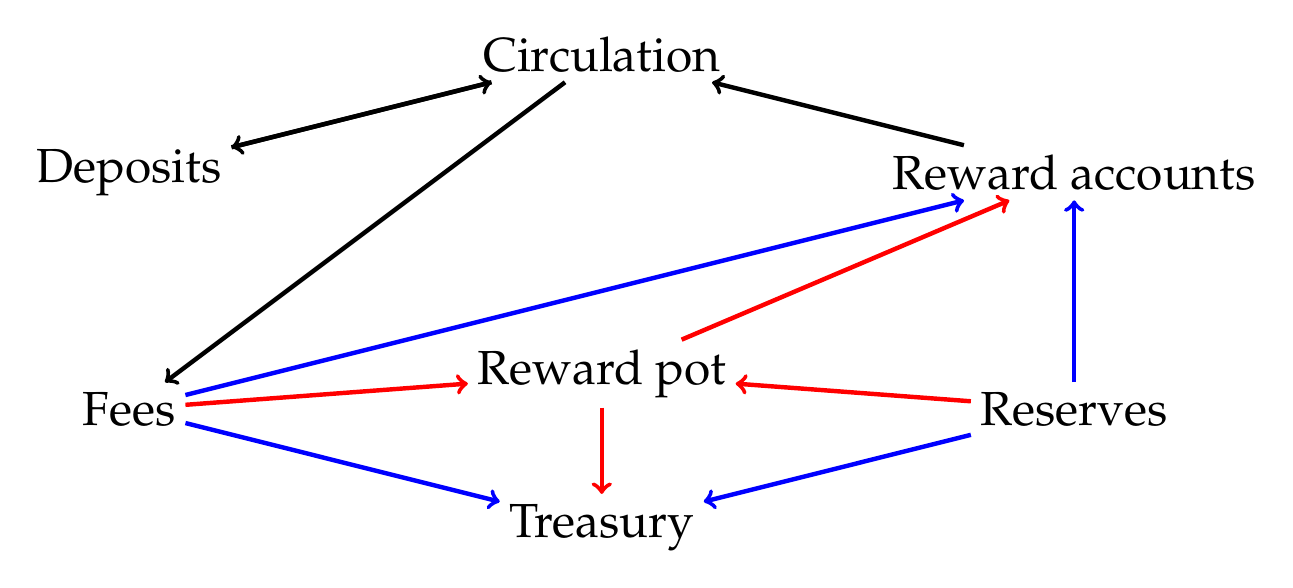
\begin{tikzpicture}
      [ x=30mm, y=30mm
      , direct/.style={black, draw}
      , implied/.style={blue, draw}
      , toTotPot/.style={red, draw}
      ]
    \node (C) at (3,2.5) {\LARGE Circulation};
    \node (R) at (5, 1) {\LARGE Reserves};
    \node (D) at (1, 2) {\LARGE Deposits};
    \node (FR) at (1,1) {\LARGE Fees};
    \node (RA) at (5, 2) {\LARGE Reward accounts};
    \node (T) at (3,0.5) {\LARGE Treasury};

    \draw[->, direct, ultra thick]
    (C) edge (D)
    (C) edge (FR)

    (D) edge (C)

    (RA) edge (C);

    \draw[->, implied, ultra thick]
    (FR) edge (T)
    (FR) edge (RA)

    (R) edge (T)
    (R) edge (RA);

    \node (TP) at (3, 1.15) {\LARGE Reward pot};

    \draw[->, toTotPot, ultra thick]
    (FR) edge (TP)
    (R) edge (TP)

    (TP) edge (RA)
    (TP) edge (T);
    \end{tikzpicture}
  \end{center}
  \caption{Preservation of Value}
  \label{fig:fund-preservation}
\end{figure}

Figure~\ref{fig:defs:reward-update} defines a reward update.
It consists of four pots:
\begin{itemize}
  \item The change to the treasury. This will be a positive value.
  \item The change to the reserves. This will be a negative value.
  \item The map of new individual rewards (to be added to the existing rewards).
  \item The change to the fee pot. This will be a negative value.
    rewards.
\end{itemize}

%%
%% Figure - Reward Update Defs
%%
\begin{figure}[htb]
  \emph{Reward Update}
  \begin{equation*}
    \RewardUpdate =
    \left(
      \begin{array}{r@{~\in~}ll}
        \Delta t & \Coin & \text{change to the treasury} \\
        \Delta r & \Coin & \text{change to the reserves} \\
        \var{rs} & \AddrRWD\mapsto\Coin & \text{new individual rewards} \\
        \Delta f & \Coin & \text{change to the fee pot} \\
      \end{array}
    \right)
  \end{equation*}
  %
  \caption{Rewards Update type}
  \label{fig:defs:reward-update}
\end{figure}

\clearpage

Figure~\ref{fig:functions:reward-update-creation} defines two functions,
$\fun{createRUpd}$ to create a reward update and $\fun{applyRUpd}$ to apply a
reward update to an instance of $\EpochState$.

The $\fun{createRUpd}$ function does the following:
\begin{itemize}
  \item Note that for all the calculations below, we use the previous protocol parameters
    $\var{prevPp}$, which corresponds to the parameters during the epoch for which we
    are creating rewards.
  \item First we calculate the change to the reserves,
    as determined by the $\rho$ protocol parameter.
  \item Next we calculate $\var{rewardPot}$, the total amount of coin available for rewards this
    epoch, as described in section 6.4 of \cite{delegation_design}. It consists of:
    \begin{itemize}
      \item The fee pot, containing the transaction fees from the epoch.
      \item The amount of monetary expansion from the reserves, calculated above.
    \end{itemize}
    Note that the fee pot is taken from the snapshot taken at the epoch boundary.
    (See~Figure\ref{fig:rules:snapshot}).
  \item Next we calculate the proportion of the reward pot that will move to the treasury,
    as determined by the $\tau$ protocol parameter. The remaining pot is called the
    $\var{R}$, just as in section 6.5 of \cite{delegation_design}.
  \item The rewards are calculated, using the oldest stake distribution snapshot (the one
    labeled ``go'').
    As given by $\fun{maxPool}$, each pool can receive a maximal amount, determined by its
    performance.  The difference between the maximal amount and the actual amount received is
    added to the amount moved to the treasury.
  \item The fee pot will be reduced by $\var{feeSS}$.
\end{itemize}

Note that fees are not explicitly removed from any account:
the fees come from transactions paying them and are accounted for whenever
transactions are processed.

The $\fun{applyRUpd}$ function does the following:
    \begin{itemize}
      \item Adjust the treasury, reserves and fee pots by the appropriate amounts.
      \item Add each individual reward to the global reward mapping.
        We must be careful, though, not to give out rewards to accounts
        that have been deregistered after the reward update was created.
        \begin{itemize}
          \item Rewards for accounts that are still registered are added to the reward mappings.
          \item The sum of the unregistered rewards are added to the reserves.
            % TODO - We may want to add these to the treasury instead, to be consistent with our other choices.
        \end{itemize}
    \end{itemize}

These two functions will be used in the blockchain transition systems in Section~\ref{sec:chain}.
In particular,
$\fun{createRUpd}$ will be used in Equation~\ref{eq:reward-update},
and $\fun{applyRUpd}$ will be used in Equation~\ref{eq:new-epoch}.

%%
%% Figure - The Reward Update Creation
%%
\begin{figure}[htb]
  \emph{Calculation to create a reward update}
  %
  \begin{align*}
    & \fun{createRUpd} \in \N \to \BlocksMade \to \EpochState \to \Coin \to \RewardUpdate \\
    & \createRUpd{slotsPerEpoch}{b}{es}{total} = \left(
      \Delta t_1,-~\Delta r_1+\Delta r_2,~\var{rs},~-\var{feeSS}\right) \\
    & ~~~\where \\
    & ~~~~~~~(\var{acnt},~\var{ss},~\var{ls},~\var{prevPp},~\wcard) = \var{es} \\
    & ~~~~~~~(\wcard,~\wcard,~\var{pstake_{go}},~\var{feeSS}) = \var{ss}\\
    & ~~~~~~~(\var{stake},~\var{delegs},~\var{poolParams}) = \var{pstate_{go}} \\
    & ~~~~~~~(\wcard,~\var{reserves}) = \var{acnt} \\
    & ~~~~~~~\left(
      \wcard,~
      \left(
      \left(\var{rewards},~\wcard,~\wcard,~\wcard,~\wcard,~\wcard\right),~
      \wcard
      \right)
      \right) = \var{ls} \\
    & ~~~~~~~\Delta r_1 = \floor*{\min(1,\eta) \cdot (\fun{rho}~\var{prevPp}) \cdot
      \var{reserves}}
    \\
    & ~~~~~~~\eta =
      \begin{cases}
        1 & (\fun{d}~\var{prevPp})\geq 0.8 \\
        \frac{blocksMade}{\floor{(1-\fun{d}~\var{prevPp})\cdot\var{slotsPerEpoch} \cdot \ActiveSlotCoeff}}
          & \text{otherwise} \\
      \end{cases} \\
    & ~~~~~~~\var{rewardPot} = \var{feeSS} + \Delta r_1 \\
    & ~~~~~~~\Delta t_1 = \floor*{(\fun{tau}~\var{prevPp}) \cdot \var{rewardPot}} \\
    & ~~~~~~~\var{R} = \var{rewardPot} - \Delta t_1 \\
    & ~~~~~~~\var{circulation} = \var{total} - \var{reserves} \\
    & ~~~~~~~\var{rs}
      = \reward{prevPp}{b}{R}{(\dom{rewards})}{poolParams}{stake}{delegs}{circulation} \\
    & ~~~~~~~\Delta r_{2} = R - \left(\sum\limits_{\_\mapsto c\in\var{rs}}c\right) \\
    & ~~~~~~~blocksMade = \sum_{\wcard \mapsto m \in b}m
  \end{align*}

  \caption{Reward Update Creation}
  \label{fig:functions:reward-update-creation}
\end{figure}

\begin{figure}[htb]
  \emph{Applying a reward update}
  %
  \begin{align*}
      & \fun{applyRUpd} \in \RewardUpdate \to \EpochState \to \EpochState \\
      & \fun{applyRUpd}~
      \left(
        \begin{array}{c}
          \Delta t \\
          \Delta r \\
          \var{rs} \\
          \Delta f \\
        \end{array}
    \right)
      \left(
        \begin{array}{c}
          \var{treasury} \\
          \var{reserves} \\
          ~ \\
          \var{rewards} \\
          \var{delegations} \\
          \var{ptrs} \\
          \var{genDelegs} \\
          \var{fGenDelegs} \\
          \var{i_{rwd}}
          \\~ \\
          \var{poolParams} \\
          \var{fPoolParams} \\
          \var{retiring} \\
          ~ \\
          \var{utxo} \\
          \var{deposited} \\
          \var{fees} \\
          \var{up} \\
          ~ \\
          \var{prevPp} \\
          \var{pp} \\
        \end{array}
      \right)
      =
      \left(
        \begin{array}{c}
          \varUpdate{\var{treasury} + \Delta t + \var{unregRU'}}\\
          \varUpdate{\var{reserves} + \Delta r}\\
          ~ \\
          \varUpdate{\var{rewards}\unionoverridePlus\var{regRU}} \\
          \var{delegations} \\
          \var{ptrs} \\
          \var{genDelegs} \\
          \var{fGenDelegs} \\
          \var{i_{rwd}}
          \\~ \\
          \var{poolParams} \\
          \var{fPoolParams} \\
          \var{retiring} \\
          ~ \\
          \var{utxo} \\
          \var{deposited} \\
          \varUpdate{\var{fees}+\Delta f} \\
          \var{up} \\
          ~ \\
          \var{prevPp} \\
          \var{pp} \\
        \end{array}
    \right) \\
    & ~~~\where \\
    & ~~~~~~~\var{regRU}=(\dom{rewards})\restrictdom rs\\
    & ~~~~~~~\var{unregRU}=(\dom{rewards})\subtractdom rs\\
    & ~~~~~~~\var{unregRU'}=\sum\limits_{\wcard\mapsto c\in\var{unregRU}} \var{c}\\
  \end{align*}

  \caption{Reward Update Application}
  \label{fig:functions:reward-update-application}
\end{figure}

\clearpage


\section{Blockchain layer}
\label{sec:chain}

This chapter introduces the view of the blockchain layer as required for the
ledger. This includes in particular the information required for the epoch
boundary and its rewards calculation as described in Section~\ref{sec:epoch}. It
also covers the transitions that keep track of produced blocks in order to
calculate rewards and penalties for stake pools.

The main transition rule is $\mathsf{CHAIN}$ which calls the subrules
$\mathsf{NEWEPOCH}$ and $\mathsf{UPDN}$, $\mathsf{VRF}$ and $\mathsf{BBODY}$.

\subsection{Block Definitions}
\label{sec:defs-blocks}

\begin{figure*}[htb]
  \emph{Abstract types}
  %
  \begin{equation*}
    \begin{array}{r@{~\in~}lr}
      \var{h} & \HashHeader & \text{hash of a block header}\\
      \var{hb} & \HashBBody & \text{hash of a block body}\\
      \var{bn} & \BlockNo & \text{block number}\\
    \end{array}
  \end{equation*}
  %
  \emph{Operational Certificate}
  %
  \begin{equation*}
    \OCert =
    \left(
      \begin{array}{r@{~\in~}lr}
        \var{vk_{hot}} & \VKeyEv & \text{operational (hot) key}\\
        \var{n} & \N & \text{certificate issue number}\\
        c_0 & \KESPeriod & \text{start KES period}\\
        \sigma & \Sig & \text{cold key signature}\\
      \end{array}
    \right)
  \end{equation*}
  %
  \emph{Block Header Body}
  %
  \begin{equation*}
    \BHBody =
    \left(
      \begin{array}{r@{~\in~}lr}
        \var{prev} & \HashHeader^? & \text{hash of previous block header}\\
        \var{vk} & \VKey & \text{block issuer}\\
        \var{vrfVk} & \VKey & \text{VRF verification key}\\
        \var{blockno} & \BlockNo & \text{block number}\\
        \var{slot} & \Slot & \text{block slot}\\
        \eta & \Seed & \text{nonce}\\
        \var{prf}_{\eta} & \Proof & \text{nonce proof}\\
        \ell & \unitInterval & \text{leader election value}\\
        \var{prf_{\ell}} & \Proof & \text{leader election proof}\\
        \var{bsize} & \N & \text{size of the block body}\\
        \var{bhash} & \HashBBody & \text{block body hash}\\
        \var{oc} & \OCert & \text{operational certificate}\\
        \var{pv} & \ProtVer & \text{protocol version}\\
      \end{array}
    \right)
  \end{equation*}
  %
  \emph{Block Types}
  %
  \begin{equation*}
    \begin{array}{r@{~\in~}l@{\qquad=\qquad}l}
      \var{bh}
      & \BHeader
      & \BHBody \times \Sig
      \\
      \var{b}
      & \Block
      & \BHeader \times \seqof{\Tx}
    \end{array}
  \end{equation*}
  \emph{Abstract functions}
  %
  \begin{equation*}
    \begin{array}{r@{~\in~}lr}
      \bhHash{} & \BHeader \to \HashHeader
                   & \text{hash of a block header} \\
      \bHeaderSize{} & \BHeader \to \N
                   & \text{size of a block header} \\
      \bBodySize{} & \seqof{\Tx} \to \N
                   & \text{size of a block body} \\
      \slotToSeed{} & \Slot \to \Seed
                    & \text{convert a slot to a seed} \\
      \prevHashToNonce{} & \HashHeader^? \to \Seed
                    & \text{convert an optional header hash to a seed} \\
      \fun{bbodyhash} & \seqof{\Tx} \to \HashBBody \\
    \end{array}
  \end{equation*}
  %
  \emph{Accessor Functions}
  \begin{equation*}
    \begin{array}{r@{~\in~}l@{~~~~~~~~~~}r@{~\in~}lr}
      \fun{bheader} & \Block \to \BHeader &
      \fun{bhbody} & \BHeader \to \BHBody \\
      \fun{hsig} & \BHeader \to \Sig &
      \fun{bbody} & \Block \to \seqof{\Tx} \\
      \fun{bvkcold} & \BHBody \to \VKey &
      \fun{bvkvrf} & \BHBody \to \VKey \\
      \fun{bprev} & \BHBody \to \HashHeader^? &
      \fun{bslot} & \BHBody \to \Slot \\
      \fun{bblockno} & \BHBody \to \BlockNo &
      \fun{bnonce} & \BHBody \to \Seed \\
      \fun{\bprfn{}} & \BHBody \to \Proof &
      \fun{bleader} & \BHBody \to \N \\
      \fun{\bprfl{}} & \BHBody \to \Proof &
      \fun{hBbsize} & \BHBody \to \N \\
      \fun{bhash} & \BHBody \to \HashBBody &
      \fun{bocert} & \BHBody \to \OCert \\
    \end{array}
  \end{equation*}
  %
  \caption{Block Definitions}
  \label{fig:defs:blocks}
\end{figure*}

\clearpage

\subsection{MIR Transition}
\label{sec:mir-trans}

The transition which moves the instantaneous rewards is $\mathsf{MIR}$.
Figure~\ref{fig:ts-types:mir} defines the types for the transition.
It has no environment or signal, and the state is $\EpochState$.

\begin{figure}
  \emph{MIR Transitions}
  \begin{equation*}
    \vdash \var{\_} \trans{mir}{} \var{\_} \subseteq
    \powerset (\EpochState \times \EpochState)
  \end{equation*}
  \caption{MIR transition-system types}
  \label{fig:ts-types:mir}
\end{figure}

Figure~\ref{fig:rules:mir} defines the MIR state transition.

If the reserve and treasury pots are large enough to cover the sum
of the corresponding instantaneous rewards,
the reward accounts are increased by the appropriate amount
and the two pots are decreased appropriately.
In either case, if the pots are large enough or not,
we reset both of the instantaneous reward mappings back to the empty mapping.

\begin{figure}[ht]
  \begin{equation}\label{eq:mir}
    \inference[MIR]
    {
      (\var{rewards},~\var{delegations},~
      \var{ptrs},~\var{fGenDelegs},~\var{genDelegs},~\var{i_{rwd}})
        \leteq \var{ds}
      \\
      (\var{treasury},~\var{reserves})\leteq\var{acnt}
      &
      (\var{irReserves},~\var{irTreasury})\leteq\var{i_{rwd}}
      \\~\\
      \var{irwdR}\leteq
        \left\{
        \fun{addr_{rwd}}~\var{hk}\mapsto\var{val}
        ~\vert~\var{hk}\mapsto\var{val}\in(\dom{rewards})\restrictdom\var{irReserves}
        \right\}
      \\
      \var{irwdT}\leteq
        \left\{
        \fun{addr_{rwd}}~\var{hk}\mapsto\var{val}
        ~\vert~\var{hk}\mapsto\var{val}\in(\dom{rewards})\restrictdom\var{irTreasury}
        \right\}
      \\~\\
      \var{totR}\leteq\sum\limits_{\wcard\mapsto v\in\var{irwdR}}v
      &
      \var{totT}\leteq\sum\limits_{\wcard\mapsto v\in\var{irwdT}}v
      \\
      \var{enough}\leteq
          \var{totR}\leq\var{reserves}
          \land\var{totT}\leq\var{treasury}
      \\
      \var{acnt'}\leteq
      {\begin{cases}
          (\var{treasury}-\var{totT},~\var{reserves}-\var{totR})
          & \var{enough}
          \\
          \var{acnt}
          &
          \text{otherwise}
       \end{cases}}
      \\~\\
      \var{rewards'}\leteq
      {\begin{cases}
          \var{rewards}\unionoverridePlus\var{irwdR}\unionoverridePlus\var{irwdT}
          & \var{enough}
          \\
          \var{rewards}
          &
          \text{otherwise}
       \end{cases}}
      \\
      \var{ds'} \leteq
      (\varUpdate{\var{rewards}'},~\var{delegations},~
      \var{ptrs},~\var{fGenDelegs},~\var{genDelegs},
      ~(\varUpdate{\emptyset},~\varUpdate{\emptyset}))
    }
    {
      \vdash
      {\left(\begin{array}{c}
            \var{acnt} \\
            \var{ss} \\
            (\var{us},~(\var{ds},~\var{ps})) \\
            \var{prevPP} \\
            \var{pp} \\
      \end{array}\right)}
      \trans{mir}{}
      {\left(\begin{array}{c}
            \varUpdate{\var{acnt'}} \\
            \var{ss} \\
            (\var{us},~(\varUpdate{\var{ds'}},~\var{ps})) \\
            \var{prevPP} \\
            \var{pp} \\
      \end{array}\right)}
    }
  \end{equation}

  \caption{MIR rules}
  \label{fig:rules:mir}
\end{figure}

\subsection{New Epoch Transition}
\label{sec:new-epoch-trans}

For the transition to a new epoch ($\mathsf{NEWEPOCH}$), the environment is
given in Figure~\ref{fig:ts-types:newepoch}, it consists of

\begin{itemize}
\item The current slot.
\item The set of genesis keys.
\end{itemize}
The new epoch state is given in Figure~\ref{fig:ts-types:newepoch}, it consists
of

\begin{itemize}
\item The number of the last epoch.
\item The information about produced blocks for each stake pool during the previous epoch.
\item The information about produced blocks for each stake pool during the current epoch.
\item The old epoch state.
\item An optional rewards update.
\item The stake pool distribution of the epoch.
\end{itemize}

\begin{figure}
  \emph{New Epoch states}
  \begin{equation*}
    \NewEpochState =
    \left(
      \begin{array}{r@{~\in~}lr}
        \var{e_\ell} & \Epoch & \text{last epoch} \\
        \var{b_{prev}} & \BlocksMade & \text{blocks made last epoch} \\
        \var{b_{cur}} & \BlocksMade & \text{blocks made this epoch} \\
        \var{es} & \EpochState & \text{epoch state} \\
        \var{ru} & \RewardUpdate^? & \text{reward update} \\
        \var{pd} & \PoolDistr & \text{pool stake distribution} \\
      \end{array}
    \right)
  \end{equation*}
  %
  \emph{New Epoch Transitions}
  \begin{equation*}
    \vdash \var{\_} \trans{newepoch}{\_} \var{\_} \subseteq
    \powerset (\NewEpochState \times \Epoch \times \NewEpochState)
  \end{equation*}
  %
  \emph{Helper function}
  \begin{align*}
      & \fun{calculatePoolDistr} \in \Snapshot \to \PoolDistr \\
      & \fun{calculatePoolDistr}~(\var{stake},~\var{delegs},~\var{poolParams}) = \\
      & ~~~\left\{\var{hk_p}\mapsto(\sigma,~\fun{poolVRF}~\var{p})
            ~\Big\vert~
            {
              \begin{array}{r@{~\in~}l}
                \var{hk_p}\mapsto\sigma & \var{sd} \\
                \var{hk_p}\mapsto\var{p} & \var{poolParams}
              \end{array}
            }
            \right\}\\
      & ~~~~\where \\
      & ~~~~~~~~~\var{total} = \sum_{\_ \mapsto c\in\var{stake}} c \\
      & ~~~~~~~~~\var{sd} = \fun{aggregate_{+}}~\left(\var{delegs}^{-1}\circ
                     \left\{\left(
                       \var{hk}, \frac{\var{c}}{\var{total}}
                     \right) \vert (\var{hk},
                     \var{c}) \in \var{stake}
                     \right\}\right) \\
  \end{align*}

  \caption{NewEpoch transition-system types}
  \label{fig:ts-types:newepoch}
\end{figure}

Figure~\ref{fig:rules:new-epoch} defines the new epoch state transition. It has three rules.
The first rule describes the change in the case of $e$ being equal to the next epoch $e_\ell+ 1$.
It also calls the $\mathsf{MIR}$ and $\mathsf{EPOCH}$ rules and checks that the reward update
is net neutral with respect to the Ada in the system.
This should always hold (by the definition of the $\fun{createRUpd}$ function)
and is present only for extra assurance and for help in proving
that Ada is preserved by this transition.
The second rule deals with the case when the epoch signal $e$ is not one greater than the
current epoch \var{e_\ell}. This rule does not change the state.
The third rule is nearly the same as the first rule, only there is no reward update to apply.
This third rule is defined for completeness, but in practice we hope that it is never used,
since it only applies in the case that epoch $e$ processed no blocks after the first
$\StabilityWindow$-many slots.

In the first case, the new epoch state is updated as follows:

\begin{itemize}
\item The epoch is set to the new epoch $e$.
\item The mapping for the blocks produced by each stake pool for the previous epoch
  is set to the current such mapping.
\item The mapping for the blocks produced by each stake pool for the current epoch
  is set to the empty map.
\item The epoch state is updated with: first applying the rewards update \var{ru},
  then calling the $\mathsf{MIR}$ transition, and finally by calling the
  $\mathsf{EPOCH}$ transition.
\item The rewards update is set to \Nothing.
\item The new pool distribution \var{pd}' is calculated from the delegation map and
  stake allocation of the previous epoch.
\end{itemize}

\begin{figure}[ht]
  \begin{equation}\label{eq:new-epoch}
    \inference[New-Epoch]
    {
      e = e_\ell + 1
      &
      \var{ru} \neq \Nothing
      &
      (\Delta t,~\Delta r,~\var{rs},~\Delta f)\leteq\var{ru}
      \\
      \Delta t+~\Delta r+\left(\sum\limits_{\wcard\mapsto v\in\var{rs}} v\right)+\Delta f=0
      \\
      \var{es'}\leteq\fun{applyRUpd}~\var{ru}~\var{es}
      &
      {
        \vdash
        \var{es'}
          \trans{\hyperref[fig:rules:mir]{mir}}{}\var{es''}
      }
      &
      {
        \vdash
        \var{es''}
          \trans{\hyperref[fig:rules:epoch]{epoch}}{\var{e}}\var{es'''}
      }
      \\~\\
      {\begin{array}{r@{~\leteq~}l}
         (\var{acnt},~\var{ss},~\wcard,~\wcard,~\wcard) & \var{es'''} \\
         (\wcard,~\var{pstake_{set}},~\wcard,~\wcard) & \var{ss} \\
         \var{pd'} & \fun{calculatePoolDistr}~\var{pstake_{set}} \\
       \end{array}}
    }
    {
      \vdash
      {\left(\begin{array}{c}
            \var{e_\ell} \\
            \var{b_{prev}} \\
            \var{b_{cur}} \\
            \var{es} \\
            \var{ru} \\
            \var{pd} \\
      \end{array}\right)}
      \trans{newepoch}{\var{e}}
      {\left(\begin{array}{c}
            \varUpdate{\var{e}} \\
            \varUpdate{\var{b_{cur}}} \\
            \varUpdate{\emptyset} \\
            \varUpdate{\var{es'''}} \\
            \varUpdate{\Nothing} \\
            \varUpdate{\var{pd}'} \\
      \end{array}\right)}
    }
  \end{equation}

  \nextdef

  \begin{equation}\label{eq:not-new-epoch}
    \inference[Not-New-Epoch]
    {
      (e_\ell,~\wcard,~\wcard,~\wcard,~\wcard,~\wcard,~\wcard)\leteq\var{nes}
      &
      e \neq e_\ell + 1
    }
    {
      \vdash\var{nes}\trans{newepoch}{\var{e}} \var{nes}
    }
  \end{equation}

  \nextdef

  \begin{equation}\label{eq:no-reward-update}
    \inference[No-Reward-Update]
    {
      (e_\ell,~\wcard,~\wcard,~\wcard,~\var{ru},~\wcard,~\wcard)\leteq\var{nes}
      &
      e = e_\ell + 1
      &
      \var{ru} = \Nothing
      \\
      {
        \vdash
        \var{es}
          \trans{\hyperref[fig:rules:mir]{mir}}{}\var{es''}
      }
      &
      {
        \vdash
        \var{es''}
          \trans{\hyperref[fig:rules:epoch]{epoch}}{\var{e}}\var{es'''}
      }
      \\~\\
      {\begin{array}{r@{~\leteq~}l}
         (\var{acnt},~\var{ss},~\wcard,~\wcard,~\wcard) & \var{es'''} \\
         (\wcard,~\var{pstake_{set}},~\wcard,~\wcard) & \var{ss} \\
         \var{pd'} & \fun{calculatePoolDistr}~\var{pstake_{set}} \\
       \end{array}}
    }
    {
      \vdash
      {\left(\begin{array}{c}
            \var{e_\ell} \\
            \var{b_{prev}} \\
            \var{b_{cur}} \\
            \var{es} \\
            \var{ru} \\
            \var{pd} \\
      \end{array}\right)}
      \trans{newepoch}{\var{e}}
      {\left(\begin{array}{c}
            \varUpdate{\var{e}} \\
            \varUpdate{\var{b_{cur}}} \\
            \varUpdate{\emptyset} \\
            \varUpdate{\var{es'''}} \\
            \var{ru} \\
            \varUpdate{\var{pd}'} \\
      \end{array}\right)}
    }
  \end{equation}
  \caption{New Epoch rules}
  \label{fig:rules:new-epoch}
\end{figure}

\clearpage

\subsection{Tick Nonce Transition}
\label{sec:tick-nonce-trans}

The Tick Nonce Transition is responsible for updating the epoch nonce and the
previous epoch's hash nonce at the start of an epoch. Its environment is shown in
Figure~\ref{fig:ts-types:ticknonce} and consists of the protocol parameters
$\var{pp}$, the candidate nonce $\eta_c$ and the previous epoch's last block
header hash as a nonce. Its state consists of the epoch nonce $\eta_0$ and
the previous epoch's last block header hash nonce.

\begin{figure}
  \emph{Tick Nonce environments}
  \begin{equation*}
    \TickNonceEnv =
    \left(
      \begin{array}{r@{~\in~}lr}
        \var{pp} & \PParams & \text{protocol parameters} \\
        \eta_c & \Seed & \text{candidate nonce} \\
        \eta_\var{ph} & \Seed & \text{previous header hash as nonce} \\
      \end{array}
    \right)
  \end{equation*}
  %
  \emph{Tick Nonce states}
  \begin{equation*}
    \TickNonceState =
    \left(
      \begin{array}{r@{~\in~}lr}
        \eta_0 & \Seed & \text{epoch nonce} \\
        \eta_h & \Seed & \text{seed generated from hash of previous epoch's last block header} \\
      \end{array}
    \right)
  \end{equation*}
  \label{fig:ts-types:ticknonce}
\end{figure}

The signal to the transition rule $\mathsf{TICKN}$ is a marker indicating
whether we are in a new epoch. If we are in a new epoch, we update the epoch
nonce and the previous hash. Otherwise, we do nothing.

\begin{figure}[ht]
  \begin{equation}\label{eq:tick-nonce-notnewepoch}
   \inference[Not-New-Epoch]
   { }
   {
     {\begin{array}{c}
        \var{pp} \\
        \eta_c \\
        \eta_\var{ph} \\
      \end{array}}
     \vdash
     {\left(\begin{array}{c}
           \eta_0 \\
           \eta_h \\
     \end{array}\right)}
     \trans{tickn}{\mathsf{False}}
     {\left(\begin{array}{c}
           \eta_0 \\
           \eta_h \\
     \end{array}\right)}
   }
 \end{equation}

 \nextdef

 \begin{equation}\label{eq:tick-nonce-newepoch}
   \inference[New-Epoch]
   {
     \eta_e \leteq \fun{extraEntropy}~\var{pp}
   }
   {
     {\begin{array}{c}
        \var{pp} \\
        \eta_c \\
        \eta_\var{ph} \\
      \end{array}}
     \vdash
     {\left(\begin{array}{c}
           \eta_0 \\
           \eta_h \\
     \end{array}\right)}
     \trans{tickn}{\mathsf{True}}
     {\left(\begin{array}{c}
           \varUpdate{\eta_c \seedOp \eta_h \seedOp \eta_e} \\
           \varUpdate{\eta_\var{ph}} \\
     \end{array}\right)}
   }
 \end{equation}

 \caption{Tick Nonce rules}
 \label{fig:rules:tick-nonce}
\end{figure}

\subsection{Update Nonce Transition}
\label{sec:update-nonces-trans}

The Update Nonce Transition updates the nonces until the randomness gets fixed.
The environment is shown in Figure~\ref{fig:ts-types:updnonce} and consists of
the block nonce $\eta$.
The update nonce state is shown in Figure~\ref{fig:ts-types:updnonce} and consists of
the candidate nonce $\eta_c$ and the evolving nonce $\eta_v$.

\begin{figure}
  \emph{Update Nonce environments}
  \begin{equation*}
    \UpdateNonceEnv =
    \left(
      \begin{array}{r@{~\in~}lr}
        \eta & \Seed & \text{new nonce} \\
      \end{array}
    \right)
  \end{equation*}
  %
  \emph{Update Nonce states}
  \begin{equation*}
    \UpdateNonceState =
    \left(
      \begin{array}{r@{~\in~}lr}
        \eta_v & \Seed & \text{evolving nonce} \\
        \eta_c & \Seed & \text{candidate nonce} \\
      \end{array}
    \right)
  \end{equation*}
  %
  \emph{Update Nonce Transitions}
  \begin{equation*}
    \_ \vdash \var{\_} \trans{updn}{\_} \var{\_} \subseteq
    \powerset (\UpdateNonceEnv
               \times \UpdateNonceState
               \times \Slot
               \times \UpdateNonceState
              )
  \end{equation*}
  \caption{UpdNonce transition-system types}
  \label{fig:ts-types:updnonce}
\end{figure}

The transition rule $\mathsf{UPDN}$ takes the slot \var{s} as signal. There are
two different cases for $\mathsf{UPDN}$: one where \var{s} is not yet
\StabilityWindow{} slots from the beginning of the next epoch and one where
\var{s} is less than \StabilityWindow{} slots until the start of the next epoch.

Note that in \ref{eq:update-both}, the nonce candidate $\eta_c$ transitions to
$\eta_v\seedOp\eta$, not $\eta_c\seedOp\eta$. The reason for this is that even
though the nonce candidate is frozen sometime during the epoch, we want the two
nonces to again be equal at the start of a new epoch (so that the entropy added
near the end of the epoch is not discarded).

\begin{figure}[ht]

  \begin{equation}\label{eq:update-both}
    \inference[Update-Both]
    {
      s < \fun{firstSlot}~((\epoch{s}) + 1) - \StabilityWindow
    }
    {
      {\begin{array}{c}
         \eta \\
       \end{array}}
      \vdash
      {\left(\begin{array}{c}
            \eta_v \\
            \eta_c \\
      \end{array}\right)}
      \trans{updn}{\var{s}}
      {\left(\begin{array}{c}
            \varUpdate{\eta_v\seedOp\eta} \\
            \varUpdate{\eta_v\seedOp\eta} \\
      \end{array}\right)}
    }
  \end{equation}

  \nextdef

  \begin{equation}\label{eq:only-evolve}
    \inference[Only-Evolve]
    {
      s \geq \fun{firstSlot}~((\epoch{s}) + 1) - \StabilityWindow
    }
    {
      {\begin{array}{c}
         \eta \\
       \end{array}}
      \vdash
      {\left(\begin{array}{c}
            \eta_v \\
            \eta_c \\
      \end{array}\right)}
      \trans{updn}{\var{s}}
      {\left(\begin{array}{c}
            \varUpdate{\eta_v\seedOp\eta} \\
            \eta_c \\
      \end{array}\right)}
    }
  \end{equation}
  \caption{Update Nonce rules}
  \label{fig:rules:update-nonce}
\end{figure}

\subsection{Reward Update Transition}
\label{sec:reward-update-trans}

The Reward Update Transition calculates a new $\RewardUpdate$ to apply in a
$\mathsf{NEWEPOCH}$ transition. The environment is shown in
Figure~\ref{fig:ts-types:reward-update}, it consists of the produced blocks
mapping \var{b} and the epoch state \var{es}. Its state is an optional reward
update.

\begin{figure}
  \emph{Reward Update environments}
  \begin{equation*}
    \RUpdEnv =
    \left(
      \begin{array}{r@{~\in~}lr}
        \var{b} & \BlocksMade & \text{blocks made} \\
        \var{es} & \EpochState & \text{epoch state} \\
      \end{array}
    \right)
  \end{equation*}
  %
  \emph{Reward Update Transitions}
  \begin{equation*}
    \_ \vdash \var{\_} \trans{rupd}{\_} \var{\_} \subseteq
    \powerset (\RUpdEnv \times \RewardUpdate^? \times \Slot \times \RewardUpdate^?)
  \end{equation*}
  \caption{Reward Update transition-system types}
  \label{fig:ts-types:reward-update}
\end{figure}

The transition rules are shown in Figure~\ref{fig:rules:reward-update}. There
are three cases, one which computes a new reward update, one which leaves the
rewards update unchanged as it has not yet been applied and finally one that
leaves the reward update unchanged as the transition was started too early.

The signal of the transition rule $\mathsf{RUPD}$ is the slot \var{s}. The
execution of the transition role is as follows:

\begin{itemize}
\item If the current reward update \var{ru} is empty and \var{s} is greater than
  the sum of the first slot of its epoch and the duration \RandomnessStabilisationWindow, then a
  new rewards update is calculated and the state is updated.
  (Note the errata in Section~\ref{sec:errata:stability-windows}.)
\item If the current reward update \var{ru} is not \Nothing, i.e., a reward
  update has already been calculated but not yet applied, then the state is not updated.
\item If the current reward update \var{ru} is empty and \var{s} is less than or equal to the sum
  of the first slot of its epoch and the duration to start rewards \RandomnessStabilisationWindow,
  then the state is not updated.
\end{itemize}

\begin{figure}[ht]
  \begin{equation}\label{eq:reward-update}
    \inference[Create-Reward-Update]
    {
      s > \fun{firstSlot}~(\epoch{s}) + \RandomnessStabilisationWindow
      &
      ru = \Nothing
      \\~\\
      ru' \leteq \createRUpd{\SlotsPerEpoch}{b}{es}{\MaxLovelaceSupply}
    }
    {
      {\begin{array}{c}
         \var{b} \\
         \var{es} \\
       \end{array}}
      \vdash
      \var{ru}\trans{rupd}{\var{s}}\varUpdate{\var{ru}'}
    }
  \end{equation}

  \nextdef

  \begin{equation}\label{eq:reward-update-exists}
    \inference[Reward-Update-Exists]
    {
      ru \neq \Nothing
    }
    {
      {\begin{array}{c}
         \var{b} \\
         \var{es} \\
       \end{array}}
      \vdash
      \var{ru}\trans{rupd}{\var{s}}\var{ru}
    }
  \end{equation}

  \nextdef

  \begin{equation}\label{eq:reward-too-early}
    \inference[Reward-Too-Early]
    {
      ru = \Nothing
      \\
      s \leq \fun{firstSlot}~(\epoch{s}) + \RandomnessStabilisationWindow
    }
    {
      {\begin{array}{c}
         \var{b} \\
         \var{es} \\
       \end{array}}
      \vdash
      \var{ru}\trans{rupd}{\var{s}}\var{ru}
    }
  \end{equation}

  \caption{Reward Update rules}
  \label{fig:rules:reward-update}
\end{figure}

\subsection{Chain Tick Transition}
\label{sec:tick-trans}

The Chain Tick Transition performs some chain level
upkeep. The environment consists of a set of genesis keys, and the state is the
epoch specific state necessary for the $\mathsf{NEWEPOCH}$ transition.

Part of the upkeep is updating the genesis key delegation mapping
according to the future delegation mapping.
For each genesis key, we adopt the most recent delegation in $\var{fGenDelegs}$
that is past the current slot, and any future genesis key delegations past the current
slot is removed. The helper function $\fun{adoptGenesisDelegs}$ accomplishes the update.

\begin{figure}
  \emph{Chain Tick Transitions}
  \begin{equation*}
    \vdash \var{\_} \trans{tick}{\_} \var{\_} \subseteq
    \powerset (\NewEpochState \times \Slot \times \NewEpochState)
  \end{equation*}
  \caption{Tick transition-system types}
  \label{fig:ts-types:tick}
  %
  \emph{helper function}
  \begin{align*}
      & \fun{adoptGenesisDelegs} \in \EpochState \to \Slot \to EpochState
      \\
      & \fun{adoptGenesisDelegs}~\var{es}~\var{slot} = \var{es'}
      \\
      & ~~~~\where
      \\
      & ~~~~~~~~~~
      (\var{acnt},~\var{ss},(\var{us},(\var{ds},\var{ps})),~\var{prevPp},~\var{pp})
      \leteq\var{es}
      \\
      & ~~~~~~~~~~
      (~\var{rewards},~\var{delegations},~\var{ptrs},
      ~\var{fGenDelegs},~\var{genDelegs},~\var{i_{rwd}})\leteq\var{ds}
      \\
      & ~~~~~~~~~~\var{curr}\leteq
        \{
          (\var{s},~\var{gkh})\mapsto(\var{vkh},~\var{vrf})\in\var{fGenDelegs}
          ~\mid~
          \var{s}\leq\var{slot}
        \}
      \\
      & ~~~~~~~~~~\var{fGenDelegs'}\leteq
          \var{fGenDelegs}\setminus\var{curr}
      \\
      & ~~~~~~~~~~\var{genDelegs'}\leteq
          \left\{
            \var{gkh}\mapsto(\var{vkh},~\var{vrf})
            ~\mathrel{\Bigg|}~
            {
              \begin{array}{l}
                (\var{s},~\var{gkh})\mapsto(\var{vkh},~\var{vrf})\in\var{curr}\\
                \var{s}=\max\{s'~\mid~(s',~\var{gkh})\in\dom{\var{curr}}\}
              \end{array}
            }
          \right\}
      \\
      & ~~~~~~~~~~\var{ds'}\leteq
          (\var{rewards},~\var{delegations},~\var{ptrs},
          ~\var{fGenDelegs'},~\var{genDelegs}\unionoverrideRight\var{genDelegs'},~\var{i_{rwd}})
      \\
      & ~~~~~~~~~~\var{es'}\leteq
      (\var{acnt},~\var{ss},(\var{us},(\var{ds'},\var{ps})),~\var{prevPp},~\var{pp})
  \end{align*}
\end{figure}

The $\mathsf{TICK}$ transition rule is shown in Figure~\ref{fig:rules:tick}.
The signal is a slot \var{s}.

Three transitions are done:

\begin{itemize}
  \item The $\mathsf{NEWEPOCH}$ transition performs any state change needed if it is the first
    block of a new epoch.
  \item The $\mathsf{RUPD}$ creates the reward update if it is late enough in the epoch.
    \textbf{Note} that for every block header, either $\mathsf{NEWEPOCH}$ or $\mathsf{RUPD}$
    will be the identity transition, and so, for instance, it does not matter if $\mathsf{RUPD}$
    uses $\var{nes}$ or $\var{nes}'$ to obtain the needed state.
\end{itemize}

\begin{figure}[ht]
  \begin{equation}\label{eq:tick}
    \inference[Tick]
    {
      {
        \vdash
        \var{nes}
        \trans{\hyperref[fig:rules:new-epoch]{newepoch}}{\epoch{slot}}
        \var{nes}'
      }
      \\~\\
      (\wcard,~\var{b_{prev}},~\wcard,~\var{es},~\wcard,~\wcard)\leteq\var{nes} \\
      \\~\\
      {
        {\begin{array}{c}
           \var{b_{prev}} \\
           \var{es} \\
         \end{array}}
        \vdash \var{ru'}\trans{\hyperref[fig:rules:reward-update]{rupd}}{\var{slot}} \var{ru''}
      }
      \\~\\
      (\var{e_\ell'},~\var{b_{prev}'},~\var{b_{cur}'},~\var{es'},~\var{ru'},~\var{pd'})
      \leteq\var{nes'}
      \\
      \var{es''}\leteq\fun{adoptGenesisDelegs}~\var{es'}~\var{slot}
      \\
      \var{nes''}\leteq
      (\var{e_\ell'},~\var{b_{prev}'},~\var{b_{cur}'},~\var{es''},~\var{ru''},~\var{pd'})
      \\~\\
    }
    {
      \vdash\var{nes}\trans{tick}{\var{slot}}\varUpdate{\var{nes''}}
    }
  \end{equation}
  \caption{Tick rules}
  \label{fig:rules:tick}
\end{figure}

\clearpage

\subsection{Operational Certificate Transition}
\label{sec:oper-cert-trans}

The Operational Certificate Transition environment consists of the genesis key
delegation map $\var{genDelegs}$ and the set of stake pools $\var{stpools}$. Its state
is the mapping of operation certificate issue numbers.  Its signal is a block
header.

\begin{figure}
  \emph{Operational Certificate environments}
  \begin{equation*}
    \OCertEnv =
    \left(
      \begin{array}{r@{~\in~}lr}
        \var{stpools} & \powerset{\type{KeyHash}} & \text{stake pools} \\
        \var{genDelegs} & \powerset{\type{KeyHash}} & \text{genesis key delegates}\\
      \end{array}
    \right)
  \end{equation*}
  %
  \emph{Operational Certificate Transitions}
  \begin{equation*}
    \var{\_} \vdash \var{\_} \trans{ocert}{\_} \var{\_} \subseteq
    \powerset (\OCertEnv \times \KeyHash_{pool} \mapsto \N \times \BHeader \times \KeyHash_{pool} \mapsto \N)
  \end{equation*}
  %
  \emph{Operational Certificate helper function}
  \begin{align*}
      & \fun{currentIssueNo} \in \OCertEnv \to (\KeyHash_{pool} \mapsto \N)
                                           \to \KeyHash_{pool}
                                           \to \N^? \\
      & \fun{currentIssueNo}~(\var{stpools}, \var{genDelegs})~ \var{cs} ~\var{hk} =
      \begin{cases}
        \var{hk}\mapsto \var{n} \in \var{cs} & n \\
        \var{hk} \in \var{stpools} & 0 \\
        \var{hk} \in \var{genDelegs} & 0 \\
        \text{otherwise} & \Nothing
      \end{cases}
  \end{align*}
  \caption{OCert transition-system types}
  \label{fig:ts-types:ocert}
\end{figure}

The transition rule is shown in Figure~\ref{fig:rules:ocert}. From the block
header body \var{bhb} we first extract the following:

\begin{itemize}
  \item The operational certificate, consisting of the hot key \var{vk_{hot}},
    the certificate issue number \var{n}, the KES period start \var{c_0} and the cold key
  signature.
\item The cold key \var{vk_{cold}}.
\item The slot \var{s} for the block.
\item The number of KES periods that have elapsed since the start period on the certificate.
\end{itemize}

Using this we verify the preconditions of the operational certificate state
transition which are the following:

\begin{itemize}
\item The KES period of the slot in the block header body must be greater than or equal to
  the start value \var{c_0} listed in the operational certificate,
  and less than $\MaxKESEvo$-many KES periods after \var{c_0}.
  The value of $\MaxKESEvo$ is the agreed-upon lifetime of an operational certificate,
  see \cite{delegation_design}.
\item \var{hk} exists as key in the mapping of certificate issues numbers to a KES
  period \var{m} and that period is less than or equal to \var{n}.
\item The signature $\tau$ can be verified with the cold verification key
  \var{vk_{cold}}.
\item The KES signature $\sigma$ can be verified with the hot verification key
  \var{vk_{hot}}.
\end{itemize}

After this, the transition system updates the operational certificate state by
updating the mapping of operational certificates where it overwrites the entry
of the key \var{hk} with the KES period \var{n}.

\begin{figure}[ht]
  \begin{equation}\label{eq:ocert}
    \inference[OCert]
    {
      (\var{bhb},~\sigma)\leteq\var{bh}
      &
      (\var{vk_{hot}},~n,~c_{0},~\tau) \leteq \bocert{bhb}
      &
      \var{vk_{cold}} \leteq \bvkcold{bhb}
      \\
      \var{hk} \leteq \hashKey{vk_{cold}}
      &
      \var{s}\leteq\bslot{bhb}
      &
      t \leteq \kesPeriod{s} - c_0
      \\~\\
      c_0 \leq \kesPeriod{s} < c_0 + \MaxKESEvo
      \\
      \fun{currentIssueNo} ~ \var{oce} ~ \var{cs} ~ \var{hk} = m
      &
      m \leq n
      \\~\\
      \mathcal{V}_{\var{vk_{cold}}}{\serialised{(\var{vk_{hot}},~n,~c_0)}}_{\tau}
      &
      \mathcal{V}^{\mathsf{KES}}_{vk_{hot}}{\serialised{bhb}}_{\sigma}^{t}
      \\
    }
    {
      \var{oce}\vdash\var{cs}
      \trans{ocert}{\var{bh}}\varUpdate{\var{cs}\unionoverrideRight\{\var{hk}\mapsto n\}}
    }
  \end{equation}
  \caption{OCert rules}
  \label{fig:rules:ocert}
\end{figure}

The OCERT rule has six predicate failures:
\begin{itemize}
\item If the KES period is less than the KES period start in the certificate,
  there is a \emph{KESBeforeStart} failure.
\item If the KES period is greater than or equal to the KES period end (start +
  $\MaxKESEvo$) in the certificate, there is a \emph{KESAfterEnd} failure.
\item If the period counter in the original key hash counter mapping is larger
  than the period number in the certificate, there is a \emph{CounterTooSmall}
  failure.
\item If the signature of the hot key, KES period number and period start is
  incorrect, there is an \emph{InvalidSignature} failure.
\item If the KES signature using the hot key of the block header body is
  incorrect, there is an \emph{InvalideKesSignature} failure.
\item If there is no entry in the key hash to counter mapping for the cold key,
  there is a \emph{NoCounterForKeyHash} failure.
\end{itemize}

\subsection{Verifiable Random Function}
\label{sec:verif-rand-funct}

In this section we define a function $\fun{vrfChecks}$ which performs all the VRF related checks
on a given block header body.
In addition to the block header body, the function requires the epoch nonce,
the stake distribution (aggregated by pool), and the active slots coefficient from the protocol
parameters. The function checks:

\begin{itemize}
\item The validity of the proofs for the leader value and the new nonce.
\item The verification key is associated with relative stake $\sigma$ in the stake distribution.
\item The $\fun{bleader}$ value of \var{bhb} indicates a possible leader for
  this slot. The function $\fun{checkLeaderVal}$ is defined in \ref{sec:leader-value-calc}.
\end{itemize}

\begin{figure}
  \emph{VRF helper function}
  \begin{align*}
      & \fun{issuerIDfromBHBody} \in \BHBody \to \KeyHash_{pool} \\
      & \fun{issuerIDfromBHBody} = \hashKey{} \circ \bvkcold{} \\
  \end{align*}
  %
  \begin{align*}
      & \fun{mkSeed} \in \Seed \to \Slot \to \Seed \to \Seed \\
      & \fun{mkSeed}~\var{ucNonce}~\var{slot}~\eta_0 =
        \var{ucNonce}~\mathsf{XOR}~(\slotToSeed{slot}\seedOp\eta_0)\\
  \end{align*}
  %
  \begin{align*}
      & \fun{vrfChecks} \in \Seed \to \BHBody \to \Bool \\
      & \fun{vrfChecks}~\eta_0~\var{bhb} = \\
      & \begin{array}{cl}
        ~~~~ &
        \verifyVrf{\Seed}{\var{vrfK}}{(\fun{mkSeed}~\Seede~\var{slot}~\eta_0)}
               {(\bprfn{bhb},~\bnonce{bhb}}) \\
        ~~~~ \land &
               \verifyVrf{\unitInterval}{\var{vrfK}}{(\fun{mkSeed}~\Seedl~\var{slot}~\eta_0)}
               {(\bprfl{bhb},~\bleader{bhb}}) \\
      \end{array} \\
      & ~~~~\where \\
      & ~~~~~~~~~~\var{slot} \leteq \bslot{bhb} \\
      & ~~~~~~~~~~\var{vrfK} \leteq \fun{bvkvrf}~\var{bhb} \\
  \end{align*}
  %
  \begin{align*}
      & \fun{praosVrfChecks} \in \Seed \to \PoolDistr \to \unitIntervalNonNull \to \BHBody \to \Bool \\
      & \fun{praosVrfChecks}~\eta_0~\var{pd}~\var{f}~\var{bhb} = \\
      & \begin{array}{cl}
        ~~~~ & \var{hk}\mapsto (\sigma,~\var{vrfHK})\in\var{pd} \\
        ~~~~ \land & \var{vrfHK} = \hashKey{vrfK} \\
        ~~~~ \land & \fun{vrfChecks}~\eta_0~\var{bhb} \\
        ~~~~ \land & \fun{checkLeaderVal}~(\fun{bleader}~\var{bhb})~\sigma~\var{f} \\
      \end{array} \\
      & ~~~~\where \\
      & ~~~~~~~~~~\var{hk} \leteq \fun{issuerIDfromBHBody}~\var{bhb} \\
      & ~~~~~~~~~~\var{vrfK} \leteq \fun{bvkvrf}~\var{bhb} \\
  \end{align*}
  %
  \begin{align*}
      & \fun{pbftVrfChecks} \in \KeyHash_{vrf} \to \Seed \to \BHBody \to \Bool \\
      & \fun{pbftVrfChecks}~\var{vrfHK}~\eta_0~~\var{bhb} = \\
      & \begin{array}{cl}
        ~~~~ & \var{vrfHK} = \hashKey{(\fun{bvkvrf}~\var{bhb})} \\
        ~~~~ \land & \fun{vrfChecks}~\eta_0~\var{bhb} \\
      \end{array} \\
  \end{align*}
  \label{fig:vrf-checks}
\end{figure}

\clearpage

\subsection{Overlay Schedule}
\label{sec:overlay-schedule}

The transition from the bootstrap era to a fully decentralized network is explained in
section 3.9.2 of~\cite{delegation_design}.
Key to this transition is a protocol parameter $d$ which controls how many slots are governed by
the genesis nodes via OBFT, and which slots are open to any registered stake pool.
The transition system introduced in this section, $\type{OVERLAY}$, covers this mechanism.

This transition is responsible for validating the protocol for both the OBFT blocks
and the Praos blocks, depending on the overlay schedule.

The actual overlay schedule itself it determined by two functions,
$\fun{isOverlaySlot}$ and $\fun{classifyOverlaySlot}$,
which are defined in Figure~\ref{fig:rules:overlay}.
The function $\fun{isOverlaySlot}$ determines if the current slot
is reserved for the OBFT nodes.
In particular, it looks at the current relative slot to
see if the next multiple of $d$ (the decentralization protocol parameter)
raises the ceiling.
If a slot is indeed in the overlay schedule,
the function $\fun{classifyOverlaySlot}$ determines if the current slot
should be a silent slot (no block is allowed) or which core node
is responsible for the block.
The non-silent blocks are the multiples of $1/\ActiveSlotCoeff$,
and the responsible core node are determined by
taking turns according the lexicographic ordering of the core node keyhashes.
\textbf{Note} that $1/\ActiveSlotCoeff$ needs to be natural number,
otherwise the multilples of $\lfloor 1/\ActiveSlotCoeff \rfloor$
will yield a different proportion of active slots than the Praos blocks.

The environments for the overlay schedule transition are:
\begin{itemize}
  \item The decentralization parameter $d$.
  \item The epoch nonce $\eta_0$.
  \item The stake pool stake distribution $\var{pd}$.
  \item The mapping $\var{genDelegs}$ of genesis keys to their cold keys and vrf keys.
\end{itemize}

The states for this transition consist only of the mapping of certificate issue numbers.

This transition establishes that a block producer is in fact authorized.
Since there are three key pairs involved (cold keys, VRF keys, and hot KES keys)
it is worth examining the interaction closely.
First we look at the regular Praos/decentralized setting,
which is given by Equation~\ref{eq:decentralized}.

\begin{itemize}
  \item First we check the operational certificate with $\mathsf{OCERT}$.
  This uses the cold verification key given in the block header.
  We do not yet trust that this key is a registered pool key.
  If this transition is successful, we know that the cold key in the block header has authorized
  the block.
\item  Next, in the $\fun{vrfChecks}$ predicate, we check that the hash of this cold key is in the
  mapping $\var{pd}$, and that it maps to $(\sigma,~\var{hk_{vrf}})$, where
  $(\sigma,~\var{hk_{vrf}})$ is the hash of the VRF key in the header.
  If $\fun{praosVrfChecks}$ returns true, then we know that the cold key in the block header was a
  registered stake pool at the beginning of the previous epoch, and that it is indeed registered
  with the VRF key listed in the header.
\item Finally, we use the VRF verification key in the header, along with the VRF proofs in the
  header, to check that the operator is allowed to produce the block.
\end{itemize}
The situation for the overlay schedule, given by Equation~\ref{eq:active-pbft}, is similar.
The difference is that we check the overlay schedule to see what core node is
supposed to make a block, and then use the genesis delegation mapping to
check the correct cold key hash and vrf key hash.

\begin{figure}
  \emph{Overlay environments}
  \begin{equation*}
    \OverlayEnv =
    \left(
      \begin{array}{r@{~\in~}lr}
        \var{d} & \{0,~1/100,~2/100,~\ldots,~1\} & \text{decentralization parameter} \\
        \var{pd} & \PoolDistr & \text{pool stake distribution} \\
        \var{genDelegs} & \GenesisDelegation & \text{genesis key delegations} \\
        \eta_0 & \Seed & \text{epoch nonce} \\
      \end{array}
    \right)
  \end{equation*}
  %
  \emph{Overlay Transitions}
  \begin{equation*}
    \_ \vdash \var{\_} \trans{overlay}{\_} \var{\_} \subseteq
    \powerset (\OverlayEnv \times (\KeyHash_{pool} \mapsto \N) \times \BHeader \times
    (\KeyHash_{pool} \mapsto \N))
  \end{equation*}
  %
  \emph{Overlay Schedule helper functions}
  \begin{align*}
      & \fun{isOverlaySlot} \in \Slot \to \unitInterval \to \Slot \to \Bool \\
      & \isOverlaySlot{fSlot}{dval}{slot} = \lceil s\cdot dval \rceil < \lceil (s+1)\cdot dval \rceil \\
      & ~~~~ \where s\leteq\slotminus{slot}{fslot}
  \end{align*}
  %
  \begin{align*}
      & \fun{classifyOverlaySlot} \in \Slot \to \powerset{\KeyHashGen} \to \unitInterval
        \to \unitIntervalNonNull \to \Slot \to \Bool \\
      & \classifyOverlaySlot{fSlot}{gkeys}{dval}{asc}{slot} = \\
      & ~~~\begin{cases}
        \fun{elemAt}~\left( \frac{\var{position}}{\var{ascInv}} \bmod |\var{gkeys}| \right)~\var{gkeys}
        &
        \text{if } \var{position} \equiv 0 \pmod{\var{ascInv}} \\
        \Nothing
        &
        \text{otherwise}
        \end{cases} \\
      & ~~~~ \where \\
      & ~~~~~~~ \var{ascInv}\leteq\lfloor 1/\var{asc}\rfloor \\
      & ~~~~~~~ \var{position}\leteq \lceil (\slotminus{slot}{fSlot})\cdot dval \rceil \\
      & ~~~~~~~ \fun{elemAt}~i~\var{set}\leteq i'\text{th lexicographic element of }\var{set}
  \end{align*}
  %
  \caption{Overlay transition-system types}
  \label{fig:ts-types:overlay}
\end{figure}

\begin{figure}[ht]
  \begin{equation}\label{eq:active-pbft}
    \inference[Active-OBFT]
    {
      \var{bhb}\leteq\bheader{bh}
      &
      \var{vk}\leteq\bvkcold{bhb}
      &
      \var{vkh}\leteq\hashKey{vk}
      \\
      \var{slot} \leteq \bslot{bhb}
      &
      \var{fSlot} \leteq \fun{firstSlot}~(\epoch{slot})
      \\
      \var{gkh}\mapsto(\var{vkh},~\var{vrfh})\in\var{genDelegs}
      \\
      \isOverlaySlot{fSlot}{(\dom{genDelegs})}{slot}\\
      \classifyOverlaySlot{fSlot}{(\dom{genDelegs})}{d}{\ActiveSlotCoeff}{slot} = \var{ghk}
      \\~\\
      \fun{pbftVrfChecks}~\var{vrfh}~\eta_0~\var{bhb}
      \\~\\
      {
        {\begin{array}{c}
         \dom{\var{pd}} \\
         \range{\var{genDelegs}} \\
         \end{array}
        }
        \vdash\var{cs}\trans{\hyperref[fig:rules:ocert]{ocert}}{\var{bh}}\var{cs'}
      }
    }
    {
      {\begin{array}{c}
         \var{d} \\
         \eta_0 \\
         \var{pd} \\
         \var{genDelegs} \\
       \end{array}}
      \vdash
      \var{cs}
      \trans{overlay}{\var{bh}}
      \varUpdate{\var{cs}'}
    }
  \end{equation}

  \nextdef

  \begin{equation}\label{eq:decentralized}
    \inference[Decentralized]
    {
      \var{bhb}\leteq\bheader{bh}
      &
      \var{slot} \leteq \bslot{bhb}
      &
      \var{fSlot} \leteq \fun{firstSlot}~(\epoch{slot})
      \\
      \neg\isOverlaySlot{fSlot}{(\dom{genDelegs})}{slot}\\
      \\~\\
      {
        \vdash\var{cs}\trans{\hyperref[fig:rules:ocert]{ocert}}{\var{bh}}\var{cs'}
      }
      \\~\\
      \fun{praosVrfChecks}~\eta_0~\var{pd}~\ActiveSlotCoeff~\var{bhb}
    }
    {
      {\begin{array}{c}
         \var{d} \\
         \eta_0 \\
         \var{pd} \\
         \var{genDelegs} \\
       \end{array}}
      \vdash
      \var{cs}
      \trans{overlay}{\var{bh}}
      \varUpdate{\var{cs}'}
    }
  \end{equation}

  \caption{Overlay rules}
  \label{fig:rules:overlay}
\end{figure}

The OVERLAY rule has nine predicate failures:
\begin{itemize}
\item If in the decentralized case the VRF key is not in the pool distribution,
  there is a \emph{VRFKeyUnknown} failure.
\item If in the decentralized case the VRF key hash does not match the one
  listed in the block header, there is a \emph{VRFKeyWrongVRFKey} failure.
\item If the VRF generated nonce in the block header does not validate
  against the VRF certificate, there is a \emph{VRFKeyBadNonce} failure.
\item If the VRF generated leader value in the block header does not validate
  against the VRF certificate, there is a \emph{VRFKeyBadLeaderValue} failure.
\item If the VRF generated leader value in the block header is too large
  compared to the relative stake of the pool, there is a \emph{VRFLeaderValueTooBig} failure.
\item In the case of the slot being in the OBFT schedule, but without genesis
  key (i.e., $Nothing$), there is a \emph{NotActiveSlot} failure.
\item In the case of the slot being in the OBFT schedule, if there is a
  specified genesis key which is not the same key as in the bock header body,
  there is a \emph{WrongGenesisColdKey} failure.
\item In the case of the slot being in the OBFT schedule, if the hash of the
  VRF key in block header does not match the hash in the genesis delegation mapping,
  there is a \emph{WrongGenesisVRFKey} failure.
\item In the case of the slot being in the OBFT schedule, if the genesis delegate
  keyhash is not in the genesis delegation mapping,
  there is a \emph{UnknownGenesisKey} failure.
  This case should never happen, and represents a logic error.

\end{itemize}

\clearpage

\subsection{Protocol Transition}
\label{sec:protocol-trans}

The protocol transition covers the common predicates of OBFT and Praos,
and then calls $\mathsf{OVERLAY}$ for the particular transitions,
followed by the transition to update the evolving and candidate nonces.

\begin{figure}
  \emph{Protocol environments}
  \begin{equation*}
    \PrtclEnv =
    \left(
      \begin{array}{r@{~\in~}lr}
        \var{d} & \{0,~1/100,~2/100,~\ldots,~1\} & \text{decentralization parameter} \\
        \var{pd} & \PoolDistr & \text{pool stake distribution} \\
        \var{dms} & \KeyHashGen\mapsto\KeyHash & \text{genesis key delegations} \\
        \eta_0 & \Seed & \text{epoch nonce} \\
      \end{array}
    \right)
  \end{equation*}
  %
  \emph{Protocol states}
  \begin{equation*}
    \PrtclState =
    \left(
      \begin{array}{r@{~\in~}lr}
        \var{cs} & \KeyHash_{pool} \mapsto \N & \text{operational certificate issues numbers} \\
        \eta_v & \Seed & \text{evolving nonce} \\
        \eta_c & \Seed & \text{candidate nonce} \\
      \end{array}
    \right)
  \end{equation*}
  %
  \emph{Protocol Transitions}
  \begin{equation*}
    \_ \vdash \var{\_} \trans{prtcl}{\_} \var{\_} \subseteq
    \powerset (\powerset{\PrtclEnv} \times \PrtclState \times \BHeader \times \PrtclState)
  \end{equation*}
  \caption{Protocol transition-system types}
  \label{fig:ts-types:prtcl}
\end{figure}

The environments for this transition are:
\begin{itemize}
  \item The decentralization parameter $d$.
  \item The stake pool stake distribution $\var{pd}$.
  \item The mapping $\var{dms}$ of genesis keys to their cold keys.
  \item The epoch nonce $\eta_0$.
\end{itemize}

The states for this transition consists of:
\begin{itemize}
  \item The operational certificate issue number mapping.
  \item The evolving nonce.
  \item The canditate nonce for the next epoch.
\end{itemize}

\begin{figure}[ht]
  \begin{equation}\label{eq:prtcl}
    \inference[PRTCL]
    {
      \eta\leteq\fun{bnonce}~(\bhbody{bhb})
      \\~\\
      {
        \eta
        \vdash
        {\left(\begin{array}{c}
        \eta_v \\
        \eta_c \\
        \end{array}\right)}
        \trans{\hyperref[fig:rules:update-nonce]{updn}}{\var{slot}}
        {\left(\begin{array}{c}
        \eta_v' \\
        \eta_c' \\
        \end{array}\right)}
      }\\~\\
      {
        {\begin{array}{c}
          \var{d} \\
          \var{pd} \\
          \var{dms} \\
          \eta_0 \\
        \end{array}
        }
        \vdash \var{cs}\trans{\hyperref[fig:rules:overlay]{overlay}}{\var{bh}} \var{cs}'
      }
    }
    {
      {\begin{array}{c}
         \var{d} \\
         \var{pd} \\
         \var{dms} \\
         \eta_0 \\
       \end{array}}
      \vdash
      {\left(\begin{array}{c}
            \var{cs} \\
            \eta_v \\
            \eta_c \\
      \end{array}\right)}
      \trans{prtcl}{\var{bh}}
      {\left(\begin{array}{c}
            \varUpdate{cs'} \\
            \varUpdate{\eta_v'} \\
            \varUpdate{\eta_c'} \\
      \end{array}\right)}
    }
  \end{equation}
  \caption{Protocol rules}
  \label{fig:rules:prtcl}
\end{figure}

The PRTCL rule has no predicate failures, besides those of the two sub-transitons.

\clearpage

\subsection{Block Body Transition}
\label{sec:block-body-trans}

The Block Body Transition updates the block body state which comprises the ledger state and the
map describing the produced blocks.
The environment of the $\mathsf{BBODY}$ transition are
the protocol parameters and the accounting state.
The environments and states are defined in Figure~\ref{fig:ts-types:bbody}, along with
a helper function $\fun{incrBlocks}$, which counts the number of non-overlay blocks
produced by each stake pool.

\begin{figure}
  \emph{BBody environments}
  \begin{equation*}
    \BBodyEnv =
    \left(
      \begin{array}{r@{~\in~}lr}
        \var{pp} & \PParams & \text{protocol parameters} \\
        \var{acnt} & \Acnt & \text{accounting state}
      \end{array}
    \right)
  \end{equation*}
  %
  \emph{BBody states}
  \begin{equation*}
    \BBodyState =
    \left(
      \begin{array}{r@{~\in~}lr}
        \var{ls} & \LState & \text{ledger state} \\
        \var{b} & \BlocksMade & \text{blocks made} \\
      \end{array}
    \right)
  \end{equation*}
  %
  \emph{BBody Transitions}
  \begin{equation*}
    \_ \vdash \var{\_} \trans{bbody}{\_} \var{\_} \subseteq
    \powerset (\BBodyEnv \times \BBodyState \times \Block \times \BBodyState)
  \end{equation*}
  \caption{BBody transition-system types}
  \label{fig:ts-types:bbody}
  %
  \emph{BBody helper function}
  \begin{align*}
      & \fun{incrBlocks} \in \Bool \to \KeyHash_{pool} \to
          \BlocksMade \to \BlocksMade \\
      & \fun{incrBlocks}~\var{isOverlay}~\var{hk}~\var{b} =
        \begin{cases}
          b & \text{if }\var{isOverlay} \\
          b\cup\{\var{hk}\mapsto 1\} & \text{if }\var{hk}\notin\dom{b} \\
          b\unionoverrideRight\{\var{hk}\mapsto n+1\} & \text{if }\var{hk}\mapsto n\in b \\
        \end{cases}
  \end{align*}

\end{figure}

The $\mathsf{BBODY}$ transition rule is shown in Figure~\ref{fig:rules:bbody},
its sub-rule is $\mathsf{LEDGERS}$ which does the update of the ledger
state. The signal is a block from which we extract:

\begin{itemize}
\item The sequence of transactions \var{txs} of the block.
\item The block header body \var{bhb}.
\item The verification key \var{vk} of the issuer of the \var{block} and its
  hash \var{hk}.
\end{itemize}

The transition is executed if the following preconditions are met:

\begin{itemize}
\item The size of the block body matches the value given in the block header body.
\item The hash of the block body matches the value given in the block header body.
\item The $\mathsf{LEDGERS}$ transition succeeds.
\end{itemize}

After this, the transition system updates the mapping of the hashed stake pool
keys to the incremented value of produced blocks (\var{n} + 1), provided the
current slot is not an overlay slot.

\begin{figure}[ht]
  \begin{equation}\label{eq:bbody}
    \inference[Block-Body]
    {
      \var{txs} \leteq \bbody{block}
      &
      \var{bhb} \leteq \bhbody{(\bheader{block})}
      &
      \var{hk} \leteq \hashKey{(\bvkcold{bhb})}
      \\~\\
      \bBodySize{txs} = \hBbsize{bhb}
      &
      \fun{bbodyhash}~{txs} = \bhash{bhb}
      \\~\\
      \\
      \var{slot} \leteq \bslot{bhb}
      &
      \var{fSlot} \leteq \fun{firstSlot}~(\epoch{slot})
      \\~\\
      {
        {\begin{array}{c}
                 \bslot{bhb} \\
                 \var{pp} \\
                 \var{acnt}
        \end{array}}
        \vdash
             \var{ls} \\
        \trans{\hyperref[fig:rules:ledger-sequence]{ledgers}}{\var{txs}}
             \var{ls}' \\
      }
    }
    {
      {\begin{array}{c}
               \var{pp} \\
               \var{acnt}
      \end{array}}
      \vdash
      {\left(\begin{array}{c}
            \var{ls} \\
            \var{b} \\
      \end{array}\right)}
      \trans{bbody}{\var{block}}
      {\left(\begin{array}{c}
            \varUpdate{\var{ls}'} \\
            \varUpdate{\fun{incrBlocks}~{\left(\isOverlaySlot{fSlot}{(\fun{d}~pp)}{slot}\right)}~{hk}~{b}} \\
      \end{array}\right)}
    }
  \end{equation}
  \caption{BBody rules}
  \label{fig:rules:bbody}
\end{figure}

The BBODY rule has two predicate failures:
\begin{itemize}
\item if the size of the block body in the header is not equal to the real size
  of the block body, there is a \emph{WrongBlockBodySize} failure.
\item if the hash of the block body is not also the hash of transactions, there is an \emph{InvalidBodyHash} failure.
\end{itemize}

\clearpage

\subsection{Chain Transition}
\label{sec:chain-trans}

The $\mathsf{CHAIN}$ transition rule is the main rule of the blockchain layer
part of the STS. It calls $\mathsf{BHEAD}$, $\mathsf{PRTCL}$, and $\mathsf{BBODY}$ as sub-rules.

The chain rule has no environment.

The transition checks six things
(via $\fun{chainChecks}$ and $\fun{prtlSeqChecks}$ from Figure~\ref{fig:funcs:chain-helper}):
\begin{itemize}
\item The slot in the block header body is larger than the last slot recorded.
\item The block number increases by exactly one.
\item The previous hash listed in the block header matches the previous
  block header hash which was recorded.
\item The size of \var{bh} is less than or equal to the maximal size that the
  protocol parameters allow for block headers.
\item The size of the block body, as claimed by the block header, is less than or equal to the
  maximal size that the protocol parameters allow for block bodies.
  It will later be verified that the size of the block body matches the size claimed
  in the header (see Figure~\ref{fig:rules:bbody}).
\item The node is not obsolete, meaning that the major component of the
  protocol version in the protocol parameters
  is not bigger than the constant $\MaxMajorPV$.
\end{itemize}


The chain state is shown in Figure~\ref{fig:ts-types:chain}, it consists of the
following:

\begin{itemize}
  \item The epoch specific state $\var{nes}$.
  \item The operational certificate issue number map $\var{cs}$.
  \item The epoch nonce $\eta_0$.
  \item The evolving nonce $\eta_v$.
  \item The candidate nonce $\eta_c$.
  \item The previous epoch hash nonce $\eta_h$.
  \item The last header hash \var{h}.
  \item The last slot \var{s_\ell}.
  \item The last block number \var{b_\ell}.
\end{itemize}

\begin{figure}
  \emph{Chain states}
  \begin{equation*}
    \LastAppliedBlock =
    \left(
      \begin{array}{r@{~\in~}lr}
        \var{b_\ell} & \Slot & \text{last block number} \\
        \var{s_\ell} & \Slot & \text{last slot} \\
        \var{h} & \HashHeader & \text{latest header hash} \\
      \end{array}
    \right)
  \end{equation*}
  %
  \begin{equation*}
    \ChainState =
    \left(
      \begin{array}{r@{~\in~}lr}
        \var{nes} & \NewEpochState & \text{epoch specific state} \\
        \var{cs} & \KeyHash_{pool} \mapsto \N & \text{operational certificate issue numbers} \\
        ~\eta_0 & \Seed & \text{epoch nonce} \\
        ~\eta_v & \Seed & \text{evolving nonce} \\
        ~\eta_c & \Seed & \text{candidate nonce} \\
        ~\eta_h & \Seed & \text{seed generated from hash of previous epoch's last block header} \\
        \var{lab} & \LastAppliedBlock^? & \text{latest applied block} \\
      \end{array}
    \right)
  \end{equation*}
  %
  \emph{Chain Transitions}
  \begin{equation*}
    \vdash \var{\_} \trans{chain}{\_} \var{\_} \subseteq
    \powerset (\ChainState \times \Block \times \ChainState)
  \end{equation*}
  \caption{Chain transition-system types}
  \label{fig:ts-types:chain}
\end{figure}

The $\mathsf{CHAIN}$ transition rule is shown in Figure~\ref{fig:rules:chain}. Its signal is a \var{block}.
The transition uses a few helper functions defined in Figure~\ref{fig:funcs:chain-helper}.

%%
%% Figure - Helper Functions for Chain Rules
%%
\begin{figure}[htb]
  \emph{Chain Transition Helper Functions}
  \begin{align*}
      & \fun{getGKeys} \in \NewEpochState \to \powerset{\KeyHashGen} \\
      & \fun{getGKeys}~\var{nes} = \dom{genDelegs} \\
      &
      \begin{array}{lr@{~=~}l}
        \where
          & (\wcard,~\wcard,~\wcard,~\var{es},~\wcard,~\wcard)
          & \var{nes}
          \\
          & (\wcard,~\wcard,~\var{ls},~\wcard,~\wcard)
          & \var{es}
          \\
          & (\wcard,~((\wcard,~\wcard,~\wcard,~\wcard,~\var{genDelegs},~\wcard),~\wcard))
          & \var{ls}
      \end{array}
  \end{align*}
  %
  \begin{align*}
      & \fun{updateNES} \in \NewEpochState \to \BlocksMade \to \LState \to \NewEpochState \\
      & \fun{updateNES}~
      (\var{e_\ell},~\var{b_{prev}},~\wcard,~(\var{acnt},~\var{ss},~\wcard,~\var{prevPp},~\var{pp}),
       ~\var{ru},~\var{pd})
          ~\var{b_{cur}}~\var{ls} = \\
      & ~~~~
      (\var{e_\ell},~\var{b_{prev}},~\var{b_{cur}},
       ~(\var{acnt},~\var{ss},~\var{ls},~\var{prevPp},~\var{pp}),~\var{ru},~\var{pd})
  \end{align*}
  %
  \begin{align*}
      & \fun{chainChecks} \in \N \to (\N,\N, \ProtVer) \to \BHeader \to \Bool \\
      & \fun{chainChecks}~\var{maxpv}~(\var{maxBHSize},~\var{maxBBSize},~\var{protocolVersion})~\var{bh} = \\
      & ~~~~ m \leq \var{maxpv} \\
      & ~~~~ \land~\bHeaderSize{bh} \leq \var{maxBHSize} \\
      & ~~~~ \land~\hBbsize{(\bhbody{bh})} \leq \var{maxBBSize} \\
      & ~~~~ \where (m,~\wcard)\leteq\var{protocolVersion}
  \end{align*}
  %
  \begin{align*}
      & \fun{lastAppliedHash} \in \LastAppliedBlock^? \to \HashHeader^? \\
      & \fun{lastAppliedHash}~\var{lab} =
        \begin{cases}
          \Nothing & lab = \Nothing \\
          h & lab = (\wcard,~\wcard,~h) \\
        \end{cases}
  \end{align*}
  %
  \begin{align*}
      & \fun{prtlSeqChecks} \to \LastAppliedBlock^? \to \BHeader \to \Bool \\
      & \fun{prtlSeqChecks}~\var{lab}~\var{bh} =
        \begin{cases}
          \mathsf{True}
          &
          lab = \Nothing
          \\
          \var{s_\ell} < \var{slot}
          \land \var{b_\ell} + 1 = \var{bn}
          \land \var{ph} = \bprev{bhb}
          &
          lab = (b_\ell,~s_\ell,~\wcard) \\
        \end{cases} \\
      & ~~~~\where \\
      & ~~~~~~~~~~\var{bhb} \leteq \bhbody{bh} \\
      & ~~~~~~~~~~\var{bn} \leteq \bblockno{bhb} \\
      & ~~~~~~~~~~\var{slot} \leteq \bslot{bhb} \\
      & ~~~~~~~~~~\var{ph} \leteq \lastAppliedHash{lab} \\
  \end{align*}

  \caption{Helper Functions used in the CHAIN transition}
  \label{fig:funcs:chain-helper}
\end{figure}

\begin{figure}[ht]
  \begin{equation}\label{eq:chain}
    \inference[Chain]
    {
      \var{bh} \leteq \bheader{block}
      &
      \var{bhb} \leteq \bhbody{bh}
      &
      \var{s} \leteq \bslot{bhb}
      \\~\\
      \fun{prtlSeqChecks}~\var{lab}~\var{bh}
      \\~\\
      {
        \vdash\var{nes}\trans{\hyperref[fig:rules:tick]{tick}}{\var{s}}\var{nes'}
      } \\~\\
      (\var{e_1},~\wcard,~\wcard,~\wcard,~\wcard,~\wcard)
        \leteq\var{nes} \\
      (\var{e_2},~\wcard,~\var{b_{cur}},~\var{es},~\wcard,~\wcard,~\var{pd})
        \leteq\var{nes'} \\
        (\var{acnt},~\wcard,\var{ls},~\wcard,~\var{pp})\leteq\var{es}\\
        ( \wcard,
          ( (\wcard,~\wcard,~\wcard,~\wcard,~\var{genDelegs},~\wcard),~
          (\wcard,~\wcard,~\wcard)))\leteq\var{ls}\\
          \var{ne} \leteq  \var{e_1} \neq \var{e_2}\\
          \eta_{ph} \leteq \prevHashToNonce{(\lastAppliedHash{lab})}
          \\~\\
          \fun{chainChecks}~
            \MaxMajorPV~(\fun{maxHeaderSize}~\var{pp},~\fun{maxBlockSize}~\var{pp},~\fun{pv}~\var{pp})~
            \var{bh}
          \\~\\
      {
        {\begin{array}{c}
        \var{pp} \\
        \eta_c \\
        \eta_\var{ph} \\
        \end{array}}
        \vdash
        {\left(\begin{array}{c}
        \eta_0 \\
        \eta_h \\
        \end{array}\right)}
        \trans{\hyperref[fig:rules:tick-nonce]{tickn}}{\var{ne}}
        {\left(\begin{array}{c}
        \eta_0' \\
        \eta_h' \\
        \end{array}\right)}
      }\\~\\~\\
      {
        {\begin{array}{c}
            (\fun{d}~\var{pp}) \\
            \var{pd} \\
            \var{genDelegs} \\
            \eta_0' \\
         \end{array}}
        \vdash
        {\left(\begin{array}{c}
              \var{cs} \\
              \eta_v \\
              \eta_c \\
        \end{array}\right)}
        \trans{\hyperref[fig:rules:prtcl]{prtcl}}{\var{bh}}
        {\left(\begin{array}{c}
              \var{cs'} \\
              \eta_v' \\
              \eta_c' \\
        \end{array}\right)}
      } \\~\\~\\
      {
        {\begin{array}{c}
                 \var{pp} \\
                 \var{acnt}
        \end{array}}
        \vdash
        {\left(\begin{array}{c}
              \var{ls} \\
              \var{b_{cur}} \\
        \end{array}\right)}
        \trans{\hyperref[fig:rules:bbody]{bbody}}{\var{block}}
        {\left(\begin{array}{c}
              \var{ls}' \\
              \var{b_{cur}'} \\
        \end{array}\right)}
      }\\~\\
      \var{nes''}\leteq\fun{updateNES}~\var{nes'}~\var{b_{cur}'},~\var{ls'} \\
      \var{lab'}\leteq (\bblockno{bhb},~\var{s},~\bhash{bh} ) \\
    }
    {
      \vdash
      {\left(\begin{array}{c}
            \var{nes} \\
            \var{cs} \\
            \eta_0 \\
            \eta_v \\
            \eta_c \\
            \eta_h \\
            \var{lab} \\
      \end{array}\right)}
      \trans{chain}{\var{block}}
      {\left(\begin{array}{c}
            \varUpdate{\var{nes}''} \\
            \varUpdate{\var{cs}'} \\
            \varUpdate{\eta_0'} \\
            \varUpdate{\eta_v'} \\
            \varUpdate{\eta_c'} \\
            \varUpdate{\eta_h'} \\
            \varUpdate{\var{lab}'} \\
      \end{array}\right)}
    }
  \end{equation}
  \caption{Chain rules}
  \label{fig:rules:chain}
\end{figure}

The CHAIN rule has six predicate failures:
\begin{itemize}
\item If the slot of the block header body is not larger than the last slot or
  greater than the current slot, there is a \emph{WrongSlotInterval} failure.
\item If the block number does not increase by exactly one,
  there is a \emph{WrongBlockNo} failure.
\item If the hash of the previous header of the block header body is not equal
  to the hash given in the environment, there is a \emph{WrongBlockSequence}
  failure.
\item If the size of the block header is larger than the maximally allowed size,
  there is a \emph{HeaderSizeTooLarge} failure.
\item If the size of the block body is larger than the maximally allowed size,
  there is a \emph{BlockSizeTooLarge} failure.
\item If the major component of the protocol version is larger than $\MaxMajorPV$,
  there is a \emph{ObsoleteNode} failure.
\end{itemize}

\clearpage

\subsection{Byron to Shelley Transition}
\label{sec:byron-to-shelley}

This section defines the valid initial Shelley ledger states and
describes how to transition the state held by the Byron ledger to Shelley.
The Byron ledger state $\CEState$ is defined in \cite{byron_chain_spec}.
The valid initial Shelley ledger states are exactly the range of
the function $\fun{initialShelleyState}$ defined in Figure~\ref{fig:functions:initial-shelley-states}.
Figure~\ref{fig:functions:to-shelley} defines the transition function from Byron.
Note that we use the hash of the final Byron header as the first evolving and
candidate nonces for Shelley.

%%
%% Figure - Shelley Initial States
%%
\begin{figure}[htb]
  \emph{Shelley Initial States}
  %
  \begin{align*}
      & \fun{initialShelleyState} \in \LastAppliedBlock^? \to \Epoch \to \UTxO
        \to \Coin \to \GenesisDelegation \\
      & ~~~ \to (\Slot\mapsto\KeyHashGen^?)
        \to \PParams \to \Seed \to \ChainState \\
      & \fun{initialShelleyState}~
      \left(
        \begin{array}{c}
          \var{lab} \\
          \var{e} \\
          \var{utxo} \\
          \var{reserves} \\
          \var{genDelegs} \\
          \var{pp} \\
          \var{initNonce} \\
        \end{array}
      \right)
      =
      \left(
        \begin{array}{c}
          \left(
            \begin{array}{c}
              \var{e} \\
              \emptyset \\
              \emptyset \\
              \left(
                \begin{array}{c}
                  \left(
                    \begin{array}{c}
                      0 \\
                      \var{reserves} \\
                    \end{array}
                  \right) \\
                  \left(
                    \begin{array}{c}
                      (\emptyset, \emptyset) \\
                      (\emptyset, \emptyset) \\
                      (\emptyset, \emptyset) \\
                      \emptyset \\
                      \emptyset \\
                      0
                    \end{array}
                  \right) \\
                  \left(
                    \begin{array}{c}
                      \left(
                        \begin{array}{c}
                          \var{utxo} \\
                          0 \\
                          0 \\
                          (\emptyset,~\emptyset) \\
                        \end{array}
                      \right) \\
                      \left(
                        \begin{array}{c}
                        \left(
                          \begin{array}{c}
                            \emptyset \\
                            \emptyset \\
                            \emptyset \\
                            \emptyset \\
                            \var{genDelegs} \\
                            \emptyset \\
                          \end{array}
                        \right) \\
                        \left(
                          \begin{array}{c}
                            \emptyset \\
                            \emptyset \\
                            \emptyset \\
                          \end{array}
                        \right) \\
                        \end{array}
                      \right) \\
                    \end{array}
                  \right) \\
                  \var{pp} \\
                  \var{pp} \\
                \end{array}
              \right) \\
              \\
              \Nothing \\
              \emptyset \\
            \end{array}
          \right) \\
          \var{cs} \\
          \var{initNonce} \\
          \var{initNonce} \\
          \var{initNonce} \\
          0_{seed} \\
          \var{lab} \\
        \end{array}
      \right) \\
      & ~~~~\where cs = \{\var{hk}\mapsto 0~\mid~(\var{hk},~\wcard)\in\range{genDelegs}\} \\
  \end{align*}

  \caption{Initial Shelley States}
  \label{fig:functions:initial-shelley-states}
\end{figure}

%%
%% Figure - Byron to Shelley State Transition
%%
\begin{figure}[htb]
  \emph{Byron to Shelley Transition}
  %
  \begin{align*}
      & \fun{toShelley} \in \CEState \to \GenesisDelegation \to \BlockNo \to \ChainState \\
      & \fun{toShelley}~
      \left(
        \begin{array}{c}
          \var{s_{last}} \\
          \wcard \\
          \var{h} \\
          (\var{utxo},~\var{reserves}) \\
          \wcard \\
          \var{us}
        \end{array}
      \right)~\var{gd}~\var{bn}
      =
      \fun{initialShelleyState}~
      \left(
        \begin{array}{c}
          (\var{s_{last}}~\var{bn},~\prevHashToNonce{h}) \\
          e \\
          \fun{hash}~{h} \\
          \var{utxo} \\
          \var{reserves} \\
          \var{gd} \\
          \overlaySchedule{e}{(\dom{gd})}{pp} \\
          \var{pp} \\
          \prevHashToNonce{h} \\
        \end{array}
      \right) \\
      & ~~~~\where \\
      & ~~~~~~~~~e = \epoch{s_{last}} \\
      & ~~~~~~~~~pp = \fun{pps}~{us} \\   % this pps function is defined in the Byron chain spec
  \end{align*}

  \caption{Byron to Shelley State Transtition}
  \label{fig:functions:to-shelley}
\end{figure}

%%% Local Variables:
%%% mode: latex
%%% TeX-master: "ledger-spec"
%%% End:

\section{Formal Properties}
\label{sec:properties}

This appendix collects the main formal properties that the new ledger rules are expected to satisfy.
Note here that in every property in this section we consider a only phase-1 valid
transactions, ie. ones that can indeed get processed.

\begin{enumerate}[label=P{\arabic*}:\ ]
\item
  \emph{Consistency with Shelley.}
  \begin{itemize}
    \item properties 15.6 - 15.16 (except 15.8 and 15.13) hold specifically in the $\fun{txValTag}~tx~=~\True$ case, because
    the calculations refer to the UTxO as if it was updated by a scripts-validating transaction
    \item other properties hold as-is
  \end{itemize}

\item
  \emph{Consistency with Multi-Asset.}
  \begin{itemize}
    \item properties 8.1 and 8.2 hold specifically in the $\fun{txValTag}~tx~=~\True$ case, because
    the calculations refer to the UTxO as if it was updated by a scripts-validating transaction
    \item other properties hold as-is
  \end{itemize}
\end{enumerate}


\begin{definition}
  For a state $s$ that is used in any subtransaction of
  $\mathsf{CHAIN}$, we define $\Utxo(s) \in \UTxO$ to be the $\UTxO$
  contained in $s$, or an empty map if it does not exist. This is
  similar to the definition of $\Val$ in the Shelley specification.

  Similarly, we also define $\field_{v}~(s)$ for the field $v$ that is part of
  the ledger state $s$, referenced by the typical variable name (eg. $\var{fees}$
  for the fee pot on the ledger).
\end{definition}

We also define a helper function $\varphi$ as follows:
\[\varphi(x, tx) :=
  \begin{cases}
    x & \fun{txValTag}~tx = \True \\
    0 & \fun{txValTag}~tx = \False
  \end{cases}\]
This function is useful to distinguish between the two
cases where a transaction can mint tokens or not, depending on whether
its scripts validate.

\begin{property}[General Accounting]
  \label{prop:pov}
  The \emph{general accounting} property in Alonzo encompasses two parts
  \begin{itemize}
    \item preservation of value property expressed via the $\fun{produced}$ and $\fun{consumed}$
    calculations, applicable for transactions with $\fun{txValTag}~tx~=~\True$, which
    is specified as in the ShelleyMA POV.
    \item the preservation of value for $\fun{txValTag}~tx~=~\False$, when
    only the collateral fees are collected into the fee pot.
  \end{itemize}

Both of these are expressed in the following lemma.

\begin{lemma}
  For all environments $e$, transactions $tx$ and states $s, s'$, if
  \begin{equation*}
    e\vdash s\trans{utxos}{tx}s'
  \end{equation*}
  then
  \begin{equation*}
    \Val(s) + \varphi(\fun{mint}~(\fun{txbody}~tx), tx) = \Val(s')
  \end{equation*}
\end{lemma}

\begin{proof}
  In the case that $\fun{txValTag}~tx = \True$ holds, the proof is
  identical to the proof of Lemma 9.1 of the multi-asset
  specification. Otherwise, the transition must have been done via the
  $\mathsf{Scripts-No}$ rule, which removes
  $\fun{collateral}~(\fun{txbody}~tx)$ from the UTxO, and increases the fee pot by the amount of the sum of Ada in the
  collateral UTxO entries. The value contained in $s$ is not changed.

  Note that in the $\fun{feesOK}$ function, there is a check that verifies
  that, in the case that there are phase-2 scripts, there are no non-Ada tokens in the UTxOs
  which the collateral inputs reference, so non-Ada tokens do not get minted, burned, or transferred
  in this case.
\end{proof}
\end{property}

\begin{property}[Extended UTxO Validation]
  \label{prop:fees-only}

  If a phase-1 valid transaction extends the UTxO, all its scripts validate
  (i.e. $\fun{txValTag}~tx = \True$).

  If a transaction is accepted and marked as paying collateral only
  (i.e. $\fun{txValTag}~tx = \False$), then the only change to the ledger
  when processing the transaction is that the collateral inputs
  are moved to the fee pot. In particular, it does not extend the UTxO.

  \begin{lemma}
    For all environments $e$, transactions $tx$ and states $s, s'$, if  and
    \begin{equation*}
      e\vdash s\trans{ledger}{tx}s'
    \end{equation*}
    then
    \[\Utxo(s') \nsubseteq \Utxo(s)~\Rightarrow~\fun{txValTag}~tx = \True \]

    Also,
    \[\fun{txvaltag}~tx = \False~ \Rightarrow~\]
    \begin{itemize}
      \item $ \field_{v}~(s') = \field_{v}~(s) \text{ for all } v~\neq~{fees}, ~v~\neq~{utxo}$
      \item $\field_{fees}~(s') = \field~\var{fees}~(s) + \fun{coin}~(\Val~(\fun{collateral}~{tx} \subtractdom \Utxo(s)))$
      \item $\Utxo(s') = \fun{collateral}~{tx} \subtractdom \Utxo(s)$
    \end{itemize}
  \end{lemma}

  \begin{proof}
    A ledger UTxO update is specified explicitly only by the $\mathsf{UTXOS}$ transition,
    and propagated (ie. applied as-specified) to a chain-state update via the
    $\mathsf{UTXO}$ and $\mathsf{UTXOW}$ transitions.

    The only case in which the $\mathsf{UTXOS}$ transition adds entries to the UTxO
    map is in the $\mathsf{Scripts-No}$ rule, when $\fun{txValTag}~tx = \True$.
    Adding entries to the UTxO map implies exactly that the updated map is not a
    submap of the original, so we get that

    \[\Utxo(s') \nsubseteq \Utxo(s)~\Rightarrow~\fun{txValTag}~tx = \True \]

   In the case that $\fun{txValTag}~tx = \False$, $\mathsf{LEDGER}$ calls the rule
   that does not update $\DPState$ at all, only the $\UTxOState$. This state update is specified
   in the $\mathsf{UTXOS}$ transition (and applied via the $\mathsf{UTXO}$ and $\mathsf{UTXOW}$ transitions).

   The only parts of the state that are updated are
   \begin{itemize}
     \item the fee pot, which is increased by the amount of the sum of Ada in the
     collateral UTxO entries, and
     \item the UTxO, where the collateral entries
     are removed.
   \end{itemize}
  \end{proof}
\end {property}

\begin{property}[Validating when No NN Scripts]
  \label{prop:is-valid}

Whenever a valid transaction does not have any phase-2 scripts, its
$\fun{txValTag} = \True$.

\begin{lemma}
  For all environments $e$, transactions $tx$ and states $s, s'$ such that
  \begin{equation*}
    e\vdash s\trans{ledger}{tx}s',
  \end{equation*}
  If $\range (\fun{txscripts}~tx) \cap \ScriptPhTwo = \emptyset$
  then $\fun{txValTag} = \True$.
\end{lemma}
\begin{proof}
  With the same argument as previously, we only need to discuss the
  equivalent claim for the $\mathsf{UTXOS}$ transition. Under these
  assumptions, $\var{sLst}$ is an empty
  list. Thus $\fun{evalScripts}~sLst = \True$, and the transition rule
  had to be $\mathsf{Scripts{-}Yes}$.
\end{proof}
\end{property}

\begin{property}[Paying fees]
  \label{prop:pay-fees}

In the case that all phase-2 scripts in a transaction validate, the transaction pays
at least the minimum transaction fee amount into the fee pot. In the case that
some do not validate, it must pay at least the percentage of the minimum fee
the collateral is required to cover.

\begin{lemma}
  For all environments $e$, transactions $tx$ and states $s, s'$ such that
  \begin{equation*}
    e\vdash s\trans{ledger}{tx}s'
  \end{equation*}
  The following holds : \\
  $\field_{fees}~(s')~\geq~\field_{fees}~(s)~+
  \begin{cases}
    \fun{minfee}~{tx} & \fun{txValTag} = \True \\
    \fun{quot}~(\fun{collateralPercent}~(\field_{pp}~(s)))~*~(\fun{minfee}~{tx})~100 & \fun{txValTag} = \False\\
  \end{cases}$.
\end{lemma}
\begin{proof}
  The fee pot is updated by the $\mathsf{Scripts{-}Yes}$ and the $\mathsf{Scripts{-}No}$
  rules, one of which is necessarily called by a valid transaction via the sequence
  of transitions called in the order $\mathsf{LEDGER}, \mathsf{UTXOW}, \mathsf{UTXO}, \mathsf{UTXOS}$.

  The $\mathsf{Scripts{-}Yes}$ rule (i.e. $\fun{txValTag} = \True$)
  transfers the amount of Lovelace in the $\fun{txfee}$ field of the
  transaction to the fee pot, which is checked to be at least the $\fun{minfee}$
  by $\fun{feesOK}$ in the $\mathsf{UTXO}$ transition. So, we get

  \[\field_{fees}~(s')~=~\field_{fees}~(s)~+~\fun{txfee}~{tx}~\geq~\field_{fees}~(s)~+~\fun{minfee}~{tx}\]

  The $\mathsf{Scripts{-}No}$ rule (i.e. $\fun{txValTag} = \False$) removes the
  $\fun{collateral}$ inputs from the
  UTxO, and adds the balance of these realized inputs to the fee pot.

  \[\field_{fees}~(s')~=~field_{fees}~(s)~+~\fun{ubalance}~(\fun{collateral}~{txb} \restrictdom \var{utxo})\]

  We can conclude that $\fun{txrdmrs}$ is non-empty whenever $\fun{txValTag} = \False$
  from the following observations :
  \begin{itemize}
    \item $\fun{txValTag} = \False$ whenever $\fun{evalScripts}$ fails.
    \item $\fun{evalScripts}$ is a $\wedge$-fold over a list of scripts and
    their inputs, containing all scripts that need to be run to validate this transaction
    \item All phase-1 scripts must succeed, as this is checked in phase-1 validation (UTXOW
    rule check). Therefore,
    $\fun{evalScripts}$ encounters a failing script which is phase-2.
    \item All phase-2 scripts necessarily have an associated redeemer attached to the
    transaction (UTXOW rule check)
  \end{itemize}

  See Property~\ref{prop:fixed-inputs} for more details on what inputs $\fun{evalScripts}$ has,
  and what we can say about the outcome of its computation with respect to its inputs.

  The $\fun{feesOK}$ check enforces that if a transaction has a non-empty
  $\fun{txrdmrs}$ field, the balance of the realized collateral inputs
  (which $\field_{fees}~(s)$ is increased by as part of processing $tx$) is

  \[\fun{ubalance}~(\fun{collateral}~{txb} \restrictdom \var{utxo})~\geq~\fun{quot}~(\txfee~{txb} * (\fun{collateralPercent}~pp))~100\]

  which, since $\txfee~{txb}~\geq~\fun{minfee}~{txb}$, gives

  \[ \geq~\fun{quot}~(\fun{minfee}~{txb} * (\fun{collateralPercent}~pp))~100)) \]

  where $\fun{txbody}~{tx}~=~{txb}$. This shows that the total collateral that gets
  moved into the fee pot from the UTxO by the $\mathsf{Scripts{-}No}$ rule is at
  least the minimum transaction fee scaled by the collateral percent parameter.

  \[\field_{fees}~(s')~\geq~\field_{fees}~(s)~+~\fun{quot}~(\fun{minfee}~{txb} * (\fun{collateralPercent}~pp))~100))\]
\end{proof}

An immediate corollary to this property is that when the $\fun{collateralPercent}$ is set to 100 or more,
the transaction always pays at least the minimum fee. This, in turn, implies that it
pays at least the fee that it has stated in the $\fun{txfee}$ field.

\begin{corollary}
  For all environments $e$, transactions $tx$ and states $s, s'$ such that
  \begin{equation*}
    e\vdash s\trans{ledger}{tx}s'~~\wedge~~\fun{collateralPercent}~(\field_{pp}~(s)) \geq 100
  \end{equation*}
  The following holds :
  \[\field_{fees}~(s')~\geq~\field_{fees}~(s)~+~\fun{minfee}~{tx} \]
\end{corollary}

\begin{proof}
  In both two cases in the lemma above, the $\field_{fees}$ field in the ledger state
  is increased by at least $\fun{minfee}~{tx}$ :
  \begin{itemize}
    \item when $\fun{txValTag} = \True$, the lemma states already that
    \[\field_{fees}~(s')~\geq~\field_{fees}~(s)~+~\fun{minfee}~{tx}\]
    \item when $\fun{txValTag} = \False$, we have
    $ \field_{fees}~(s')~\geq~\field_{fees}~(s)~+~\fun{quot}~(\fun{minfee}~{txb} * (\fun{collateralPercent}~pp))~100$ \\
    $~~~\geq~\field_{fees}~(s)~+~\fun{quot}~(\fun{minfee}~{tx}~*~100)~100$ \\
    $~~~=~\field_{fees}~(s)~+~\fun{minfee}~{tx}$
  \end{itemize}
\end{proof}

\end{property}

\begin{property}[Correct tag]
  \label{prop:correct-tag}

The $\fun{txValTag}~tx$ tag of a phase-1 valid transaction must match the result of the $\fun{evalScripts}$
function for that transaction.

\begin{lemma}
  For all environments $e$, transactions $tx$ and states $s, s'$ such that
  \begin{equation*}
    e\vdash s\trans{utxos}{tx}s',
  \end{equation*}
  The following holds :
    \[\fun{txValTag}~tx ~=~ \fun{evalScripts}~{tx}~{sLst} \]
  where
  \[ \var{sLst} \leteq \fun{collectTwoPhaseScriptInputs}~\mathsf{EI}~\mathsf{SysSt} ~\field_{pp}(s)~\var{tx}~ \Utxo(s) \]
\end{lemma}
\begin{proof}
  Inspecting the $\mathsf{Scripts{-}Yes}$ and the $\mathsf{Scripts{-}No}$ rules of the $\mathsf{UTXOS}$ transition,
  we see that both the $\fun{txValTag}$ and the result of $\fun{evalScripts}$
  are $\True$ in the former, and $\False$ in the latter.
\end{proof}
\end{property}

\begin{property}[Replay protection]
  \label{prop:replay}

A transaction always removes at least one UTxO entry from the ledger, which provides
replay protection.

\begin{lemma}
  For all environments $e$, transactions $tx$ and states $s, s'$ such that
  \begin{equation*}
    e\vdash s\trans{ledger}{tx}s',
  \end{equation*}
  The following holds : $\Utxo~(s)~\nsubseteq~\Utxo~(s')$.
\end{lemma}
\begin{proof}
  The UTxO is updated by the $\mathsf{Scripts{-}Yes}$ and the $\mathsf{Scripts{-}No}$
  rules, on of which is necessarily called by a valid transaction. Both of these
  rules remove UTxOs corresponding to a set of inputs.

  In both cases, there is a check that the removed inputs set is non-empty.
  The $\mathsf{Scripts{-}Yes}$ rule of the $\mathsf{UTXOS}$ transition
  removes the UTxOs associated with the input set $\fun{txinputs}~{tx}$ from the ledger.
  The $\fun{txinputs}~{tx}$ set must be non-empty because there is a check in the
  $\mathsf{UTXO}$ rule (which calls $\mathsf{UTXOS}$) that ensure this is true.

  For the $\mathsf{Scripts{-}No}$ rule of the $\mathsf{UTXOS}$ transition
  removes the UTxOs associated with the input set $\fun{collateral}~{tx}$ from the ledger.
  The $\fun{collateral}~{tx}$ set must be non-empty because
  the $\fun{feesOK}$ function (called by the same rule that calls $\mathsf{UTXO},
  \mathsf{UTXOS}$) ensures that in the case that the $tx$ contains phase-2 scripts,
  $\fun{collateral}~{tx}$ must be non-empty.

  Note that by property~\ref{prop:is-valid}, phase-2 scripts must always be present
  if $\fun{txValTag}~tx = \False$ (that is, whenever $\mathsf{Scripts{-}No}$ rule is used).
\end{proof}
\end{property}

\begin{property}[UTxO-changing transitions]
  \label{prop:utxo-change}

The $\mathsf{UTXOS}$ transition fully specifies the change in the ledger $\UTxO$
for each transaction.

\begin{lemma}
  For all environments $e$, transitions $\mathsf{TRNS}$, transactions $tx$ and states $s, s'$ such that
  \begin{equation*}
    e\vdash s\trans{trns}{tx}s'
  \end{equation*}
  The following holds :
  \begin{equation*}
    \Utxo(s) \neq \Utxo(s')~\Rightarrow~e'\vdash u\trans{utxos}{tx}u'
  \end{equation*}
  where $\Utxo(s) = \Utxo(u)~\wedge~\Utxo(s') = \Utxo(u')$ for some environment $e'$,
  and states $u, u'$.
\end{lemma}
\begin{proof}
  By inspecting each transition in this specification, as well as those inherited from the
    Shelley one, we see that a non-trivial update from the UTxO of $s$ to that of $s'$
    must be done by $\mathsf{UTXOS}$. Every other transition that changes the UTxO and
    has a signal of type $\Tx$ only applies the $\mathsf{UTXOS}$.
\end{proof}
\end{property}

\begin{property}[Deterministic script evaluation]
  \label{prop:fixed-inputs}

The deterministic script evaluation property, also stated as
"script interpreter arguments are fixed", is a property of the Alonzo ledger
that guarantees that the outcome of phase-2 script validation in a (phase-1 valid) transaction
depends only on the contents of that transaction, and not on when, by who, or in what
block that transaction was submitted.

For this property, we make some assumptions about things that are outside the scope of this specification :

\begin{itemize}
  \item The Plutus script
  interpreter is a pure function that receives only the arguments provided by the ledger when it is
  invoked by calling the $\fun{runPLCScript}$ function. We assume that this is
  also true in an implementation. In particular, the interpreter does not
  obtain any system randomness, etc.

  \item We do not need to check here that the hashes that are the keys of the
  $\fun{txscripts}$ and $\fun{txdats}$ fields match the computed hashes of the scripts and
  datum objects they index. This is because these hashes must be computed as part of
  the deserialization of a transaction (see the CDDL specification),
  instead of being transmitted as part of the transaction and then checked. We
  assume these hashes are correct.

  \item We assume that the consensus
  function $\fun{epochInfoSlotToUTCTime}$ for converting a slot interval into a
  system time interval is deterministic.

  \item We assume that the two global
  constants, $\EpochInfo$ and $\SystemStart$, which it also takes as parameters,
  cannot change within the span of any interval for which $\fun{epochInfoSlotToUTCTime}$
  is able to convert both endpoints to system time.
\end{itemize}

The assumptions above are implicit in the functional style of definitions in this
specification, but they are worth pointing out for implementation.
With these assumptions in mind, we can say that
script evaluation is deterministic.

We split this result into a lemma and its corollary :

\begin{itemize}
  \item First, we demonstrate that all the scripts and their arguments that are
  collected for phase-2 validation are the same for two phase-1 valid transactions with the same body,
  independent of the (necessarily valid) ledger state to which they are being applied

  \item Second, we derive the corollary that under the same validity assumptions,
  phase-2 validation results in the same outcome for both transactions
\end{itemize}

\begin{lemma}
  \label{lem:inputs}
  For all environments $e, e'$, transactions $tx, tx'$ and states $s, s', u, u'$ such that
  $e$ and $s$ are subsets of fields of some valid chain state $c$, and
  $e'$ and $s'$ are subsets of fields of some valid chain state $c'$,

  \begin{equation*}
    e\vdash s\trans{ledger}{tx}s', \\
    e'\vdash u\trans{ledger}{tx'}u', \\
    \txbody{tx} = \txbody{tx'}
  \end{equation*}

  The following holds :

  \[\fun{toSet}~(\fun{collectTwoPhaseScriptInputs}~\mathsf{EI}~\mathsf{SysSt} ~\field_{pp}(s)~\var{tx}~ \Utxo(s))\]
  \[ = \]
  \[\fun{toSet}~(\fun{collectTwoPhaseScriptInputs}~\mathsf{EI}~\mathsf{SysSt} ~\field_{pp}(u)~\var{tx'}~ \Utxo(u))\]

\end{lemma}
\begin{proof}

    The $\fun{collectTwoPhaseScriptInputs}$
    function (see \ref{fig:functions:script2})
    constructs a list where each entry contains a Plutus script
    and the arguments passed to the interpreter for its evaluation.

    To show that $\fun{collectTwoPhaseScriptInputs}$ returns a list containing
    the same elements for both $tx$ and $tx'$, we observe that
    the set of elements from which this list is produced via $\fun{toList}$
    is generated using the following functions, as well as set comprehension
    and list operations.
    We demonstrate that the functions used in this definition
    produce the same output for $tx$ and $tx'$, as all the data they
    inspect is fixed by the transaction body :

    \begin{itemize}
      \item $\fun{scriptsNeeded}$ : The $\PolicyID$, $\AddrRWD$, and $\DCert$ data
      output by this function as the second term of the hash-purpose pair
      is obtained directly from the $\fun{mint}$, $\fun{txwdrls}$,
      $\fun{txcerts}$ fields of the transaction, which are all fixed by the
      body of the transaction. These types of script purposes all include
      the hash of the validating script.

      The only other data this function inspects is the UTxO entries associated
      with the $\fun{txinputs}$ (passed via the $\UTxO$ argument) to get the realized inputs.
      We know that the UTxO is a field in a valid chain state for both the phase-1 valid
      transactions $tx$ and
      the $tx'$ ($\Utxo(s)$ and $\Utxo(u)$, respectively). This means that the $\TxId$
      in each input present in either UTxO is a hash of the body of the transaction
      containing the $\TxOut$ part of the UTxO entry indexed by that input. The
      order of the outputs is also fixed by the body, which fixes the $\Ix$ of
      the entry.

      A different value in output part of the UTxO entry (or a different order of
      outputs) would necessarily imply
      that the hash of the body containing that output must be different.
      Therefore, for all Plutus script-locked realized inputs of either transaction,
      the script hash in the payment credential of the address
      (and, by the same argument, the datum hash) are fixed by the inputs in body of the
      transaction, despite not being explicitly contained in it. We then get that

      \[ \fun{scriptsNeeded}~\Utxo(s)~(\txbody{tx}) = \fun{scriptsNeeded}~\Utxo(u)~(\txbody{tx'}) \]

      \item $\fun{getDatum}$ : In the case the script purpose
      is of the input type, the datum this function returns is one that
      is associated with the corresponding realized input. More precisely, it is the datum whose
      hash is specified in the realized input, and is looked up by hash in the $\fun{txdats}$
      transaction field. If there is no datum hash in the realized input, or the script purpose
      is of a non-input type, the empty list is returned.

      The $\mathsf{UTXOW}$ rule checks that the transaction is carrying all datums corresponding
      to its realized inputs. Since the inputs (and realized inputs) are the same
      for $tx$ and $tx'$ (fixed by the body), this guarantees that
      of the datum hashes in the realized inputs (and therefore, their preimages)
      are the same as well.

      \item $\fun{txscripts}$ : in the $\mathsf{UTXOW}$ rule, there is a check that all the
      script preimages of the script hashes returned by the $\fun{scriptsNeeded}$
      function must be present in this field.

      \item $\fun{indexedRdmrs}$ : like $\fun{scriptsNeeded}$, this function
      examines four fields fixed by the transaction body ($\fun{mint}$, $\fun{txwdrls}$,
      $\fun{txcerts}$, and $\fun{txinputs}$).
      It also looks at data in the $\fun{txrdmrs}$ field, which is fixed
      by the transaction body via the $\fun{scriptIntegrityHash}$
      hash. This is done as follows: the $\mathsf{UTXOW}$ rule verifies that this
      hash-containing field matches the computed hash
      of the preimage constructed from several fields of the transaction,
      including $\fun{txrdmrs}$ (this calculation
      is done by the $\fun{hashScriptIntegrity}$ function).

      \item $\fun{language}$ : this is directly conveyed by the type of a script.

      \item $\fun{costmdls}$ : The hash calculated by the $\fun{hashScriptIntegrity}$
      function and compared to the hash value in the $\fun{scriptIntegrityHash}$ field
      must include in the preimage the current cost models of
      all script languages of scripts carried by the transaction. Recall that
      if a cost model changed between when a transaction was submitted and the
      time at which it was processed, the field and the calculated hash values
      will not match.

      \item $\fun{valContext}$ and $\fun{txInfo}$ :
      The $\fun{valContext}$ function is defined in \ref{sec:txinfo} and is pure.
      All fields of the $\TxInfo$
      structure, with the exceptions listed below,
      are straightforward translations of the corresponding transaction body fields (see \ref{sec:txinfo}) that
      are given no additional arguments,
      and therefore completely determined by $tx$ and $tx'$. The fields not directly
      appearing in the body are :

      \begin{itemize}
        \item $\fun{txInfoInputs}$ : this field contains the realized inputs of
        the transaction which are fixed by the transaction and the unique
        UTxO entries to which the inputs correspond. As explained above,
        accessing information in realized inputs for script evaluation
        does not break determinism.

        \item $\fun{txInfoValidRange}$ : this field contains the transaction
        validity interval as system time (converted from the slot numbers, which are
        used to specify the interval in the transaction body). This conversion is
        done by a function defined in the consensus layer, and takes two global
        constants in addition to the slot interval itself. Since the slot interval
        conversion function $\fun{epochInfoSlotToUTCTime}$ necessarily
        succeeds if both $tx$ and $tx'$ pass phase-1 validation, the additional
        global constant arguments must be the same (by assumption). The determinism of this conversion
        is one of the assumptions of this property, and thus gives the same output
        for both transactions.

        \item $\fun{txInfoData}$ : this field is populated with the datums (and their
        hashes) in the transaction field $\fun{txdats}$, which are fixed by the body
        via the $\fun{scriptIntegrityHash}$ field.

        \item $\fun{txInfoId}$ : this field contains the hash of the transaction body,
        which is clearly the same for transactions with the same body.
      \end{itemize}

      Therefore, each field of the $\TxInfo$ structure is
      the same for two transactions with the same body, ie.

      \[ \fun{txInfo}~\PlutusVI~\Utxo(s)~\var{tx} = \fun{txInfo}~\PlutusVI~\Utxo(u)~\var{tx'}\]

    \end{itemize}
\end{proof}

We can now make the general statement about evaluation of all scripts done in
phase-2 validation : for any phase-1 valid transactions with the same body,
the outcome of phase-2 script evaluation is the same. We make the same assumptions
as in Lemma \ref{lem:inputs}.

\begin{corollary}
  For all environments $e, e'$, transactions $tx, tx'$ and states $s, s', u, u'$ such that
  \begin{equation*}
    e\vdash s\trans{ledger}{tx}s', \\
    e'\vdash u\trans{ledger}{tx'}u', \\
    \txbody{tx} = \txbody{tx'}
  \end{equation*}
  The following holds :

  \[\fun{evalScripts}~{tx}~ (\fun{collectTwoPhaseScriptInputs}~\mathsf{EI}~\mathsf{SysSt} ~\field_{pp}(s)~\var{tx}~ \Utxo(s))\]
  \[ = \]
  \[\fun{evalScripts}~{tx'}~ (\fun{collectTwoPhaseScriptInputs}~\mathsf{EI}~\mathsf{SysSt} ~\field_{pp}(u)~\var{tx'}~ \Utxo(u))\]

\end{corollary}

\begin{proof}
  Let us consider the use of arguments of $\fun{evalScripts}$ (see Figure \ref{fig:functions:script2}).
  The first argument (of type $\Tx$) is only inspected in the case that the script $sc$ (the first element
    in the pair at the head of the list of script-arguments pairs is a phase-1 script. Since all phase-1 scripts
    are checked in phase one of validation (see \ref{fig:rules:utxow-alonzo}) by calling $\fun{validateScript}$
    on all scripts attached to the transaction. For this to apply to $sc$, we must also show
    that $sc$ is a script attached to the transaction (see the second argument explanation).
    Note also that the $tx$ argument passed to $\fun{evalScripts}$ at the use site (in the $\mathsf{UTXOS}$ transition)
    is the same, unmodified $tx$ as is the signal for the LEDGER transition. We verify this by inspecting
    the sequence of transitions through which it is propagated
    ($\mathsf{UTXOS}$, $\mathsf{UTXO}$, $\mathsf{UTXOW}$, and $\mathsf{LEDGER}$), and their signals.

    This allows us to conclude that at every step of the iteration over the script-arguments pairs list,
    the first argument to $\fun{evalScripts}$,

    \begin{itemize}
      \item has no impact on the outcome of script evaluation in the case the script
      being validated at this step is phase-2, as it is completely ignored, and,

      \item because $\fun{collectTwoPhaseScriptInputs}$ filters out all phase-1 scripts,
      is, in fact, ignored always.
    \end{itemize}

    The second argument to $\fun{evalScripts}$, ie. the list of scripts and their arguments,
    has already been shown to contain the same tuples for both transactions in the lemma above.
    The order of the list does not affect the validation outcome, since the interpreter is run
    on each tuple of a script and its arguments independently of all other tuples in the list.
    The function $\fun{evalScripts}$ is a $\wedge$-fold over the list. Thus, we may ignore the order
    of the elements in the generated list as it does not affect the evaluation outcome.

    From this we may conclude that the outcome of both phase-1 and phase-2 script evaluations
    at each step of $\fun{evalScripts}$ must be the same for $tx$ and $tx'$. Therefore,
    the $\wedge$-fold of them done by $\fun{evalScripts}$ also produces the same outcome
    for both transactions.

\end{proof}
\end{property}


\begin{enumerate}
\item
  \emph{Commutativity of Translation.} Translate, then apply to Alonzo ledger is
  the same as apply to MA ledger, then translate the ledger.
\item
  \emph{Zero ExUnits.} If a script is run (there’s a redeemer/exunits) , it will fail with 0 units
\item
  \emph{Cost Increase.} if a transaction is valid, it will remain valid if you increase the execution units
\item
  \emph{Cost Lower Bound.} if a transaction contains at least one valid script, it must have at least one execution unit
\item
  \emph{Tx backwards Compatibility.} Any transaction that was accepted in a previous version of the ledger rules
    has exactly the same cost and effect, except that the transaction output is extended.
\item \emph{Run all scripts.} All scripts attached to a transaction are run
\item
  ... \todo{Anything else?}
\end{enumerate}



\addcontentsline{toc}{section}{References}
\bibliographystyle{plainnat}
\bibliography{references}

\begin{appendix}
  \include{valmonoid-examples}
  \section{Script Constructors and Evaluation}
\label{sec:timelock-lang}


\begin{figure}[htb]
  \begin{align*}
    \fun{validateScript} & \in\Script\to\Tx\to\Bool \\
    \fun{validateScript} ~s~\var{tx}~& =~
                             \fun{evalTimelock}~\var{vhks} ~\var{itr}~\var{s} \\
                         & ~~~~\where \\
                         & ~~~~~~~~\var{vhks}\leteq \{\fun{hashKey}~vk \vert
                           vk \in \dom(\fun{txwitsVKey}~\var{tx})\} \\
                         & ~~~~~~~~\var{itr} \leteq \fun{txvldt}~ (\txbody~ \var{tx})
  \end{align*}
  \caption{Script Validation}
  \label{fig:functions-validate}
\end{figure}

In the ShelleyMA era, the
$\fun{validateScript}$ function performs validation of only timelock scripts,
see Figure~\ref{fig:functions-validate}. Note that while there is no explicit
support for validating multi-signature scripts in $\fun{validateScript}$,
these scripts remain effectively usable as the encodings of multi-sig and timelock
scripts are compatible. An existing multi-sig script-locked output is
spent by interpreting the encoded script as a timelock script (one without
any validity interval clauses), then validating it. For details, see the CDDL
specification.

The arguments that are passed to the $\fun{validateScript}$ function include all those
that are needed for $\Timelock$ script evaluation :

\begin{itemize}
\item The script getting evaluated
\item The transaction
\end{itemize}

The semantics of the Timelock language are specified in Figure~\ref{fig:defs:tx-mc-eval}.
The evaluation of the scripts constructed by $\type{Signature}, \type{AllOf},
\type{AnyOf}, \type{MOfN}$ is done the same as for their
$\ScriptNI$ counterparts. The $\type{RequireTimeStart}$ evaluation
checks that the start of the transaction validity interval is not $\Nothing$, and is in or after
the slot specified by the constructor. The $\type{RequireTimeExpire}$ evaluation
checks that the end of the transaction validity interval is not $\Nothing$, and is in or before
the slot specified by the constructor.

\begin{figure*}[htb]
  \emph{Timelock Script Constructor Types}
  \begin{align*}
    & \type{evalTimelock} & \in \powerset{\KeyHash}\to(\Slot^? \times \Slot^?)\to\Timelock \to \Bool & \\
    & \text{The type of the Timelock script evaluator} \\~\\
    %
    & \type{Signature} & \in \KeyHash \to \Timelock & \\
    %
    & \type{AllOf} & \in \seqof{\Timelock} \to \Timelock & \\
    %
    & \type{AnyOf} & \in \seqof{\Timelock} \to \Timelock & \\
    %
    & \type{MOfN} & \in \N \to \seqof{\Timelock} \to \Timelock & \\
    %
    & \type{RequireTimeStart} & \in \Slot \to \Timelock &\\
    %
    & \type{RequireTimeExpire} & \in \Slot \to \Timelock &\\
  \end{align*}
  %
  \emph{Timelock Script Evaluation}
  \begin{align*}
    \fun{evalTimelock} & ~(\type{Signature}~hk)~\var{vhks}~\wcard =  hk \in vhks \\
    \fun{evalTimelock} & ~(\type{AllOf}~ts)~\var{vhks}~\wcard =
                              \forall t \in ts: \fun{evalTimelock}~t~vhks\\
    \fun{evalTimelock} & ~(\type{AnyOf}~ts)~\var{vhks}~\wcard =
                              \exists t \in ts: \fun{evalTimelock}~t~vhks\\
    \fun{evalTimelock} & ~(\type{MOfN}~m~ts)~\var{vhks}~\wcard = \\
                             & m \leq \Sigma
                               (\textrm{card} \{ t s.t. t \leftarrow ts \wedge \fun{evalTimelock}~\var{t}~\var{vhks} \}) \\
    \fun{evalTimelock} &~(\type{RequireTimeStart}~\var{lockStart})~\var{vhks}~\var{(\var{txStart}, \wcard)} \\
    & =~
    \begin{cases}
      \False & \var{txStart} = \Nothing \\
      \var{lockStart} \leq \var{txStart} & \text{otherwise}
    \end{cases} \\
    \fun{evalTimelock} &~(\type{RequireTimeExpire}~\var{lockExp})~\var{vhks}~\var{(\wcard, \var{txExp})} \\
    & =~
    \begin{cases}
      \False & \var{txExp} = \Nothing \\
      \var{txExp} \leq \var{lockExp} & \text{otherwise}
    \end{cases} \\
  \end{align*}
  \caption{Timelock Script Constructor Types and Evaluation}
  \label{fig:defs:tx-mc-eval}
\end{figure*}

% The Figures~\ref{fig:defs:tx-mc-eval},~\ref{fig:defs:tx-mc-eval-2},
% and~\ref{fig:whitelist-example} give
% possible constructors of the Timelock language.
%
% %% \begin{note}
% %%   sort out the constructors
% %% \end{note}
%
% \begin{figure*}[htb]
%   \begin{align*}
%     & \fun{evalTimelock} \in\Timelock\to\PolicyID\to\Slot\to\powerset\KeyHash \\
%     &~~~~\to\TxBody\to\UTxO \to\Bool  \\
%     & \text{UTxO is only for the outputs THIS tx is spending, not global UTxO, i.e.} \\
%     & \text{when called,}~\var{spentouts}~=~(\fun{txins}~\var{txb}) ~\restrictdom~\var{utxo} \\~\\
%     %
%     & \fun{evalTimelock}  ~(\type{JustMSig}~s)~\var{pid}~\var{slot}~\var{vhks}
%      ~\var{txb}~\var{spentouts} \\
%     &~~~~ =~ \fun{evalMultiSigScript}~s~\var{vhks} \\
%     & \text {checks the msig script}\\~\\
%     %
%     & \fun{evalTimelock}
%      ~\type{DoMint}~\var{pid}~ \var{slot}~\var{vhks} ~\var{txb}~\var{spentouts} \\
%     &~~~~ =~ \var{pid} \notin \dom~(\fun{mint}~\var{txb}) \\
%     & \text {checks that script hash of this script is not an asset ID being minted by tx}  \\~\\
%     %
%     & \fun{evalTimelock}
%      ~\type{SignedByPIDToken}~\var{pid}~ \var{slot}~\var{vhks} ~\var{txb}~\var{spentouts} \\
%     &~~~~ =~ \exists~t\mapsto ~\_~\in~ \fun{range}~(\var{pid}~ \restrictdom~(\fun{ubalance}~\var{spentouts})) ~:~ t~\in~\var{vhks} \\
%     & \text{checks that tx is signed by a key whose hash is the name of a token in this asset}
%     \\~\\
%     & \fun{evalTimelock}
%      ~(\type{SpendsCur}~\var{pid'})~\var{pid}~ \var{slot}~\var{vhks} ~\var{txb}~\var{spentouts} \\
%     &~~~~ =~ (\var{pid'}~\neq~\Nothing ~\wedge ~\var{pid'}~\in~ \dom~(\fun{ubalance}~\var{spentouts}))\\
%     &~~~~~~ \vee (\var{pid'}~=~\Nothing ~\wedge ~\var{pid}~\in~ \dom~(\fun{ubalance}~\var{spentouts})) \\
%     & \text{checks that this transaction spends asset pid' OR itself if}~\var{pid'}~=~\Nothing
%     \\~\\
%     &\fun{evalTimelock}~(\type{Not}~s)~\var{pid}~\var{slot}~\var{vhks}
%     ~\var{txb}~\var{spentouts}
%    \\
%     &~~~~ = \neg ~\fun{evalTimelock}~s~\var{pid}~\var{slot}~\var{vhks}
%     ~\var{txb}~\var{spentouts}\\~\\
%     %
%     &\fun{evalTimelock}~(\type{RequireAll}~ls)~\var{pid}~\var{slot}~\var{vhks}
%     ~\var{txb}~\var{spentouts}
%    \\
%     &~~~~ = \forall ~s'~ \in~ ls~:~\fun{evalTimelock}~s'~\var{pid}~\var{slot}~\var{vhks}
%     ~\var{txb}~\var{spentouts}\\~\\
%     %
%     &\fun{evalTimelock}~(\type{RequireOr}~ls)~\var{pid}~\var{slot}~\var{vhks}
%     ~\var{txb}~\var{spentouts}
%    \\
%     &~~~~ = \exists ~s'~ \in~ ls~:~\fun{evalTimelock}~s'~\var{pid}~\var{slot}~\var{vhks}
%     ~\var{txb}~\var{spentouts}\\
%   \end{align*}
%   \caption{Multi-asset Script Evaluation}
%   \label{fig:defs:tx-mc-eval}
% \end{figure*}
%
% \begin{figure*}[htb]
%   \begin{align*}
%     & \fun{evalTimelock}
%      ~(\type{AssetToAddress}~\var{pid'}~\var{addr})~\var{pid}~ \var{slot}~\var{vhks} ~\var{txb}~\var{spentouts} \\
%     &~~~~ =~ \forall~(a, v)~\in~\fun{range}~(\fun{outs}~txb),~\\
%     &~~~~~~ \var{c}~\in~\dom~v~\Rightarrow~(a~=~ \var{a'} ~\wedge~
%                        v~=~\var{c}~ \restrictdom~(\fun{ubalance}~(\fun{outs}~txb)) \\
%     & \where \\
%     & ~~~~~~~ \var{a'}~=~\fun{if}~ \var{addr}~\neq~\Nothing~\fun{then}~\var{addr}~\fun{else}~\var{(pid',pid')} \\
%     & ~~~~~~~ \var{c}~=~\fun{if}~ \var{pid'}~\neq~\Nothing~\fun{then}~\var{pid'}~\fun{else}~\var{pid} \\
%     & \text{checks that tx outputs any pid tokens by themselves to the specified address} \\
%     & \text {the script address of the given asset when addr unspecified} \\~\\
%     & \fun{evalTimelock}
%      ~(\type{TrancheTokens}~\var{tts}~\var{txin})~\var{pid}~\var{slot}~\var{vhks}
%      ~\var{txb}~\var{spentouts}  \\
%     &~~~~ =~(\var{pid}\mapsto\var{tts}~\in~\var{val})~ \wedge~(\var{txin}~\in~\fun{txins}~{txb}) \\
%     & \text{tranche tokens is incomplete} \\~\\
%     %
%     & \fun{evalTimelock}
%      ~(\type{FreshTokens})~\var{pid}~\var{slot}~\var{vhks}
%      ~\var{txb}~\var{spentouts}
%       \\
%     &~~~~ =~\forall~\var{pid}~ \mapsto ~tkns ~\in~ \var{val}~:~ \\
%     &~~~~ \forall~t~\in~\var{tkns},~
%         \fun{nameToken}~(\fun{indexof}~\var{t}~\var{tkns},~\fun{txins}~{txb})~=~t
%     \end{align*}
%     \caption{Multi-asset Script Evaluation, cont.}
%     \label{fig:defs:tx-mc-eval-2}
% \end{figure*}
%
% \begin{figure*}[htb]
%   \begin{align*}
%     & \fun{whitelist} \in\ScriptMSig\to\Script  \\~\\
%     %
%     & \type{whitelist}  ~\var{msig}~ =~ \type{RequireOr}~
%       (\type{RequireAll}~(\type{DoMint};~\type{JustMSig}~\var{msig});~\\
%     &~~~~~~ \type{RequireAll}~(\type{AssetToAddress}~\Nothing~\Nothing ;\\
%     &~~~~~~ (\type{Not}~\type{DoMint});~\type{SignedByPIDToken})) \\
%     %
%     & \text{msig is some MSig script containing signatures of some accreditation authority} \\
%     & \text{i.e. this authority can do any minting or spending of this token} \\~\\
%     %
%     & (\fun{hashScript}~(\type{SpendsCur}~(\fun{hashScript}~(\type{whitelist}~\var{msig}))),~ \var{tkns}) \\
%     & \text{an example of an output spending which requires to be on a whitelist made by msig authority}
%   \end{align*}
%   \caption{Whitelist Script Example}
%   \label{fig:whitelist-example}
% \end{figure*}

  \section{Output Size}
\label{sec:value-size}

Figure \ref{fig:test} gives the formula for calculating the size of a UTxO entry
in the Alonzo era. In addition to the data found in the UTxO in the ShelleyMA
era, the hash of a datum (or $\Nothing$) is added to the output type, which
is accounted for in the size calculation.

\begin{figure*}[h]
  \emph{Constants}
  \begin{align*}
  & \mathsf{JustDataHashSize} \in \MemoryEstimate \\
  & \text{The size of a datum hash wrapped in $\DataHash^?$} \\~
  \\
  & \mathsf{NothingSize} \in \MemoryEstimate \\
  & \text{The size of $\Nothing$ wrapped in $\DataHash^?$}
  \end{align*}
  %
  \emph{Helper Functions}
  \begin{align*}
    & \fun{dataHashSize} \in \DataHash^? \to \MemoryEstimate \\
    & \fun{dataHashSize}~ \Nothing = \mathsf{NothingSize} \\
    & \fun{dataHashSize}~ \wcard = \mathsf{JustDataHashSize} \\
    & \text{Return the size of $\DataHash^?$} \\~\\
    & \fun{utxoEntrySize} \in \TxOut \to \MemoryEstimate \\
    & \fun{utxoEntrySize}~\var{(a, v, d)} = \mathsf{utxoEntrySizeWithoutVal} + (\fun{size} (\fun{getValue}~(a, v, d))) + \mathsf{dataHashSize}~d \\
    & \text{Calculate the size of a UTxO entry}
  \end{align*}
  \caption{Value Size}
  \label{fig:test}
\end{figure*}

\begin{note}
  Get dataHashSize from heapwords on the code
\end{note}

There is a change of constant value from the ShelleyMA era, specifically:

\begin{itemize}
  \item $\mathsf{adaOnlyUTxOSize} = 29$ instead of $27$
  \item $\mathsf{k_0} = 2$ instead of $0$
\end{itemize}

Additionally, the new constants used in Alonzo have values :

\begin{itemize}
  \item $\mathsf{JustDataHashSize} = 10$ words
  \item $\mathsf{NothingSize} = 0$ words
\end{itemize}

\end{appendix}

\end{document}
